\documentclass[a4paper,twoside,12pt]{book} % Openany for starting chapter on any pages

\usepackage{structure} % Code defining the structure and style of the document
%% --------------- Definition of constant --------------- %%
\newcommand{\uimla}{Český spolek horských průvodců} %Associations name
\newcommand{\logo}{
\includegraphics[width=6cm]{Figures/Logo/UIMLA-Logo.png}} % Logo of associations
\newcommand{\finalwork}{Závěrečná práce} %Final work
\newcommand{\titleCZ}{Záchranné lanové techniky s využitím kladkostojů} % Czech name of final work
\newcommand{\authorfinalwork}{Šarlota Dušková} % Author name 
\newcommand{\program}{Mezinárodní horský průvodce} % Name of program
\newcommand{\place}{Praha} % Place
\newcommand{\where}{Praze} % Place
\newcommand{\yearoffinalwork}{2022} %Year
\newcommand{\dayoffinalwork}{01.06.2022}
 % Introduction
\addto\captionsenglish{\renewcommand*\contentsname{Obsah}}
\addto{\captionsenglish}{\renewcommand{\bibname}{Seznam použité literatury}}
\usepackage{cite}
\begin{document}
%% -------------------------------------------------- %%
%% -------------------- Title page ------------------- %%
%% -------------------------------------------------- %%
\thispagestyle{empty}
\begin{titlepage}
\begin{center}
{\textbf{\large{\MakeUppercase{\uimla}}}}\\
{\color{NavyBlue}\rule{\linewidth}{0.5mm}}
\vspace{1cm} \\
\logo\\
\smallskip
{\textbf{\large{\MakeUppercase{\finalwork}}}}\\
\bigskip
{\MakeUppercase{\titleCZ}}\\
\vspace{8.0cm}
\begin{tabular}{llrl}
Program: & \program\\
\end{tabular}
\vspace{2cm} \\
\authorfinalwork \\
{\color{NavyBlue}\rule{\linewidth}{0.5mm}}
\place \space \yearoffinalwork
\end{center}
\end{titlepage}
%% -------------------------------------------------- %%
%% -------------------- Content -------------------- %%
%% -------------------------------------------------- %%
\tableofcontents
\thispagestyle{empty} % Removes numbers from last page.
%% -------------------------------------------------- %%
%% -------------------- Chapters --------------------- %%
%% -------------------------------------------------- %%
\chapter*{Úvod}
\label{Uvod}
%% -------------------------------------------------- %%
\def\figurename{Obr.} % Figure name
\def\tablename{Tab.} % Table name
\def\figureautorefname{obr.} % Autoreference 
\def\tableautorefname{tab.} % Autoreference
\def\chapterautorefname{kapitola} % Autoreference
%% -------------------------------------------------- %%
\addcontentsline{toc}{chapter}{Úvod}
Budu se zabývat problematikou záchrany ve skalním terénu. Uvedu základní potřebný materiál k záchraně (viz \autoref{Potrebny_material}). Zaměřím se na základní záchranné techniky klientů ve volném terénu či na zajištěných cestách (viz \autoref{Mozne_zpusoby_zachrany}). Výstupem bude vytvoření webové aplikace (viz \autoref{Webova_aplikace}), kde si uživatel bude moct nastavit hmotnost zachraňovaného lezce, zavést do výpočtu různé případy účinnosti kladek použitých v systému a umožní vypočítat skutečnou vytaženou délku lana k záchraně lezce o požadovanou vzdálenost. Všechny výpočty ve webové aplikaci budou shrnuty v následující kapitole (viz \autoref{Vypocty}). Cílem této aplikace bude umožnit uživateli jednoduše nasimulovat situaci a vypočítat jakou hmotnost bude muset vytáhnout, pokud jeho spolulezec či klient nebude moct překonat určitou pasáž, či se zraní a nebude moct pokračovat ve výstupu. V poslední kapitole budou uvedeny kombinace skutečných účinností kladkostrojů 3:1, 5:1 a 7:1, které mohou v reálném případě za použití běžných pomůcek nastat (viz \autoref{Souhrn}).
\chapter{Seznam potřebných věcí}
\label{Potrebny_material}
%% -------------------------------------------------- %%
\def\figurename{Obr.} % Figure name
\def\tablename{Tab.} % Table name
\def\figureautorefname{obr.} % Autoreference 
\def\tableautorefname{tab.} % Autoreference
\def\chapterautorefname{kapitola} % Autoreference
%% -------------------------------------------------- %%

Zde uvádím kompletní seznam s věcí potřebných pro přechod TMB.

\noindent\textbf{Seznam věcí na přechod:}
\begin{itemize}
    \item vlněné ponožky 4-5x
    \item kraťasy
    \item dlouhé kalhoty
    \item merino tričko 3x
    \item mikinu
    \item péřovou bundu
    \item větrovku
    \item nepromokavou bundu
    \item termo prádlo
    \item čepici
    \item kulicha
    \item nákrčník
    \item turistické boty
    \item nesmeky (pokud se jde brzy v sezóně)
    \item sluneční brýle
    \item trekingové hole
    \item batoh dle výběru přechodu:
    \begin{itemize}
    	\item přechod na lehko - 30-35 l
    	\item přechod na těžko - 50-60 l
    \end{itemize}
    \item rezervoár na vodu - 3,0 l
    \item pláštěnku na batoh
    \item vlastní lékárničku
    \item power banku
    \item cestovní ručník
    \item papírovou mapu
    \item buzolu
    \item čelovku
\end{itemize}

\noindent\textbf{Seznam věcí pro spaní na chatě:}
\begin{itemize}
    \item přezuvky
    \item vložka do spacáku nebo malý lehký spacák
    \item špunty do uší
\end{itemize}

\noindent\textbf{Seznam věcí pro spaní v kempech:}
\begin{itemize}
    \item karimatku
    \item spacák
    \item bivakovací vak a nebo stan
\end{itemize}

\noindent\textbf{Seznam hygienických přípravků:}
\begin{itemize}
    \item balzám na rty (SPF 50+)
    \item opalovací krém (SPF 50+)
    \item kartáček na zuby a cestovní zubní pastu
    \item deodorant
    \item hřeben
\end{itemize}

\noindent\textbf{Seznam základních potřeb v lékárničce:}
\begin{itemize}
    \item náplasti a compeed náplasti na puchýře
    \item kineziologická tejpa
    \item antiseptické ubrousky
    \item nůžky a pinzeta
    \item obvazy
    \item trojcípí šátek
    \item dezinfekci
    \item léky dle osobních potřeb
    \item léky na bolest (paracetamol nebo ubuprofen)
    \item hroznový cukr
    \item tužku
\end{itemize}

%\selectlanguage{czech}
\chapter{Možné způsoby záchrany}
\label{Mozne_zpusoby_zachrany}
%% -------------------------------------------------- %%
\def\figurename{Obr.} % Figure name
\def\tablename{Tab.} % Table name
\def\figureautorefname{obr.} % Autoreference 
\def\tableautorefname{tab.} % Autoreference
\def\chapterautorefname{kapitola} % Autoreference
%% -------------------------------------------------- %%

V následující kapitole si ukážeme možné způsoby záchrany. Záchranu budeme provádět pomocí kladkostroje. Kladkostroje se dělí podle účinnosti. 

\subsection*{Stanovení účinnosti kladkostroje}

Kladkostroj snižuje úsilí potřebné k vytažení záchraňovaného. 

\section{Kladkový efekt}

Budeme-li uvažovat břemeno zavěšené na laně procházející kladkou zavěšenou nad tímto břemenem, bude platit 2. Newtonův zákon "Síla působící na těleso o hmotnosti \textit{m} uvádí těleso do rovnoměrně zrychleného pohybu se zrychlením \textit{a}.", tedy jakákoliv síla působící na jeden konec lana se přenese na druhý konec lana.

Pokud břemeno zavěšené na laně váží 100\,kg, musí na druhé straně lana udržet, taktéž 100\,kg (viz~\autoref{Obr:pulley_system}). Každý pramen lana vyvine tah 100\,kg, takže kladka nese 200\,kg.

%% -------------------------------------------------- %%
%% -------------------- Picture --------------------- %%
%% -------------------------------------------------- %%
\begin{figure}[!hbt]
    \centering
    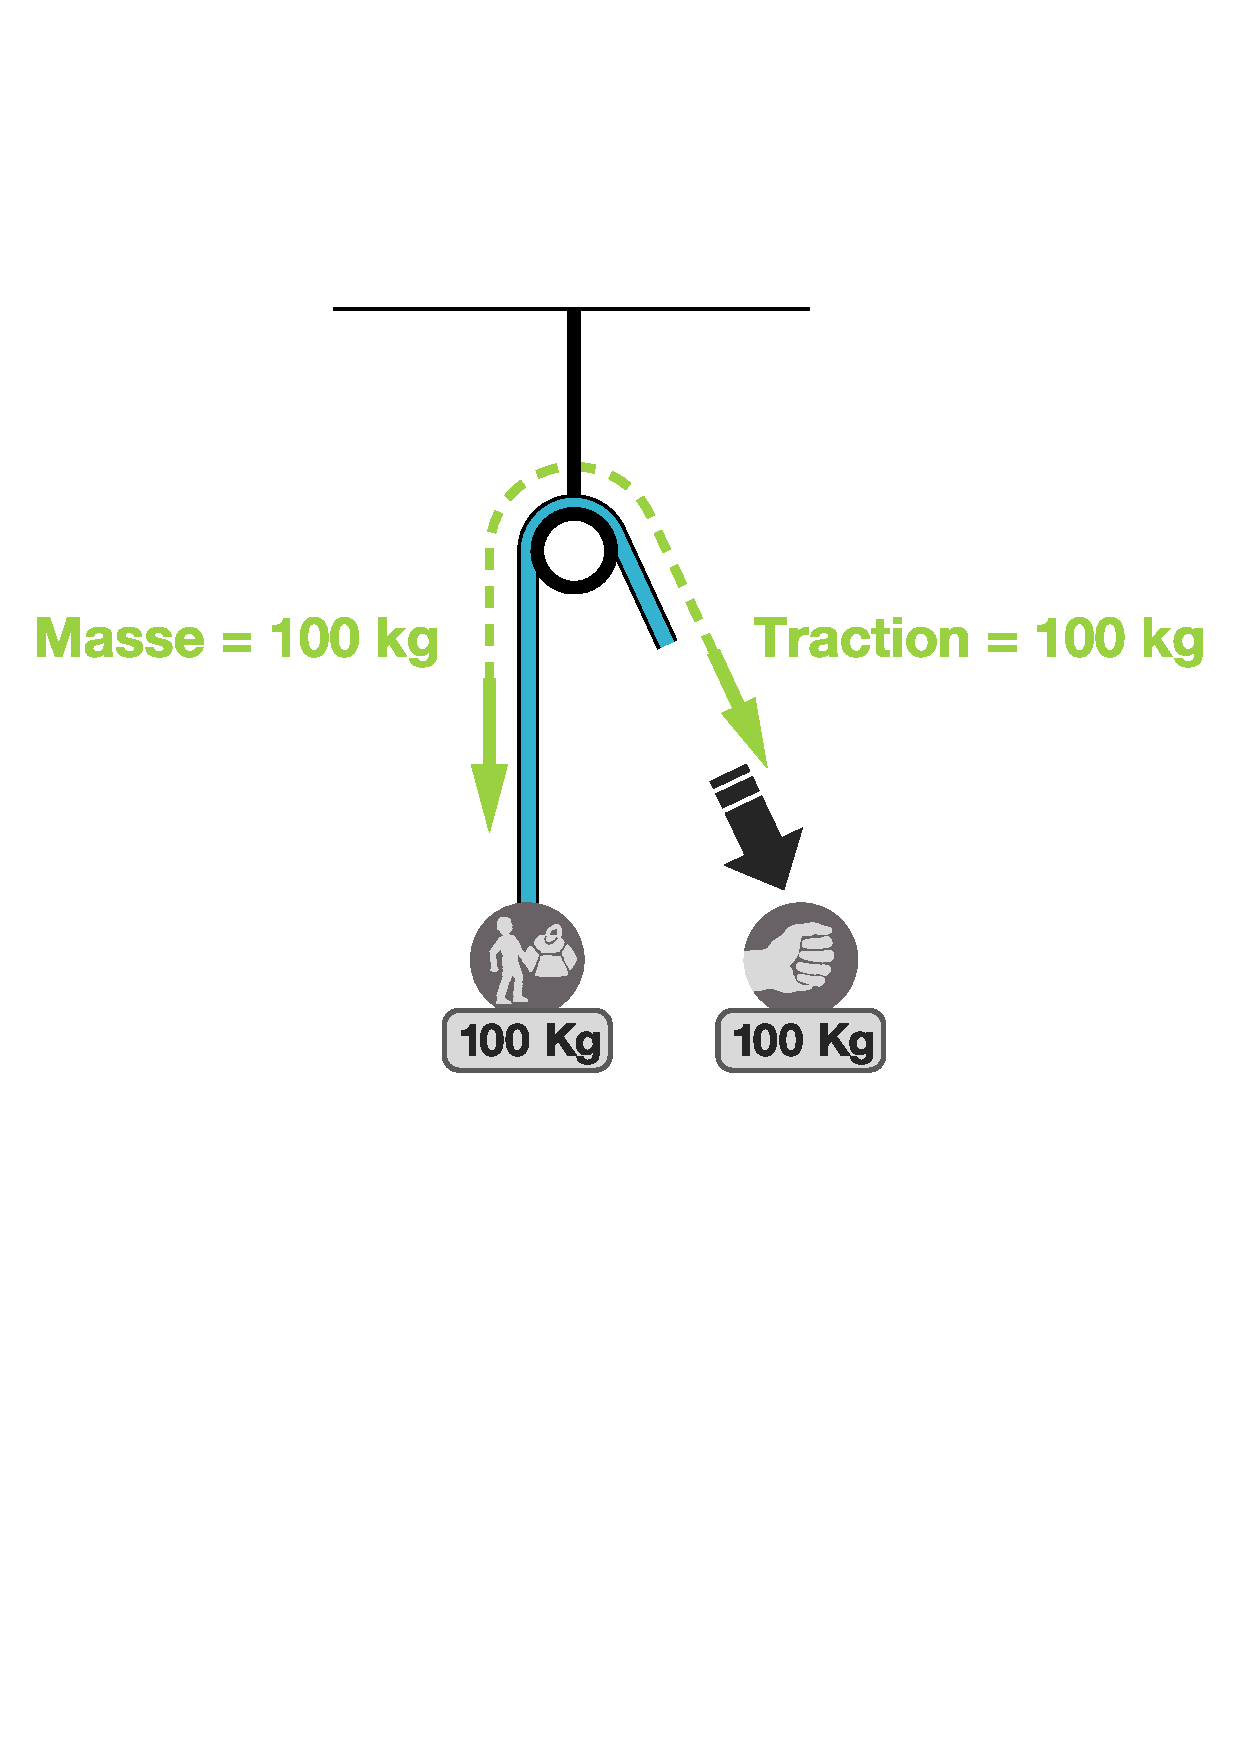
\includegraphics[width=10.0cm]{Figures/PulleySystem/pulley_system.pdf}
    \caption[Kladkový efekt]{Kladkový efekt (schéma převzato ze zdroje \cite{Petzl_2022})}
    \label{Obr:pulley_system}
\end{figure} 
%% -------------------------------------------------- %%

Tato teorie platí pouze pro ideální kladkostroj s účinností 100\%, která reálně neexistuje. Ve skutečnosti se dokážeme pohybovat v rozmezí od 50\% do 98\%. Pro zjednodušenní výpočtů budu pracovat s účinností 100\%.

Účinnost tj. síla značená (E) taženého systému udává multiplikační faktor síly, který můžeme na lano vyvinout. Pokud jsme na laně schopni utáhnout 20\,kg systém 3:1 umožní zvednou 60\,kg. Tohoto snížení se dosáhne zvýšením množství taženého lana. Uvažujeme-li ideální stav, tedy 100\% účinnost systému, potřebujeme k vytažení zátěže o 1\,m se systémem 3:1 vytáhnout 3\,m lana.

Účinnost (E) taženého systému lze vypočítat sečtením účinků každé kladky. Pokud máme kladkostroje se sudým číslem, jedná se o formu kladkostroje se zatížením ukotveným nahoře. V našem případě budeme využívat kladkostroje s lichým číslem, tedy se zatížením dole. Zaměřím se na kladkostroj 3:1, 5:1 a 7:1 \cite{Petzl_2022}.

\section{Kladkostroje}

Pro určení mechanické účinnosti systému slouží T-metoda, neboli metoda sčítání napětí. Jedná se o výpočet mechanické účinnosti lana a kladky. K určení T-metody stačí pouze následovat 4. kroky:

1. Vedle taženého lana zapíšeme T1.

2. Vedle každé kladky si zakreslíme tři čáry, tyto čáry budou značit vstup do kladky, kladku a výstup z kladky. Vždy platí rovnováha sil, tedy síly co vstoupí do kladky musí i vystoupit.

3. Doplníme prázdné řádky.

4. Po doplnění všech řádek zjistíme mechanickou účinnost systému \cite{rope_rescue_web_calculating_MA_T_system} (viz Obr. Rozložení sil).
\newpage
\subsection{Systém 1:1}
%% -------------------------------------------------- %%
%% -------------------- Pictures --------------------- %%
%% -------------------------------------------------- %%
\begin{figure}[h]
    \centering
    \subcaptionbox{Sestrojení kladkostroje\label{Obr:1:1_Pulley_system}}{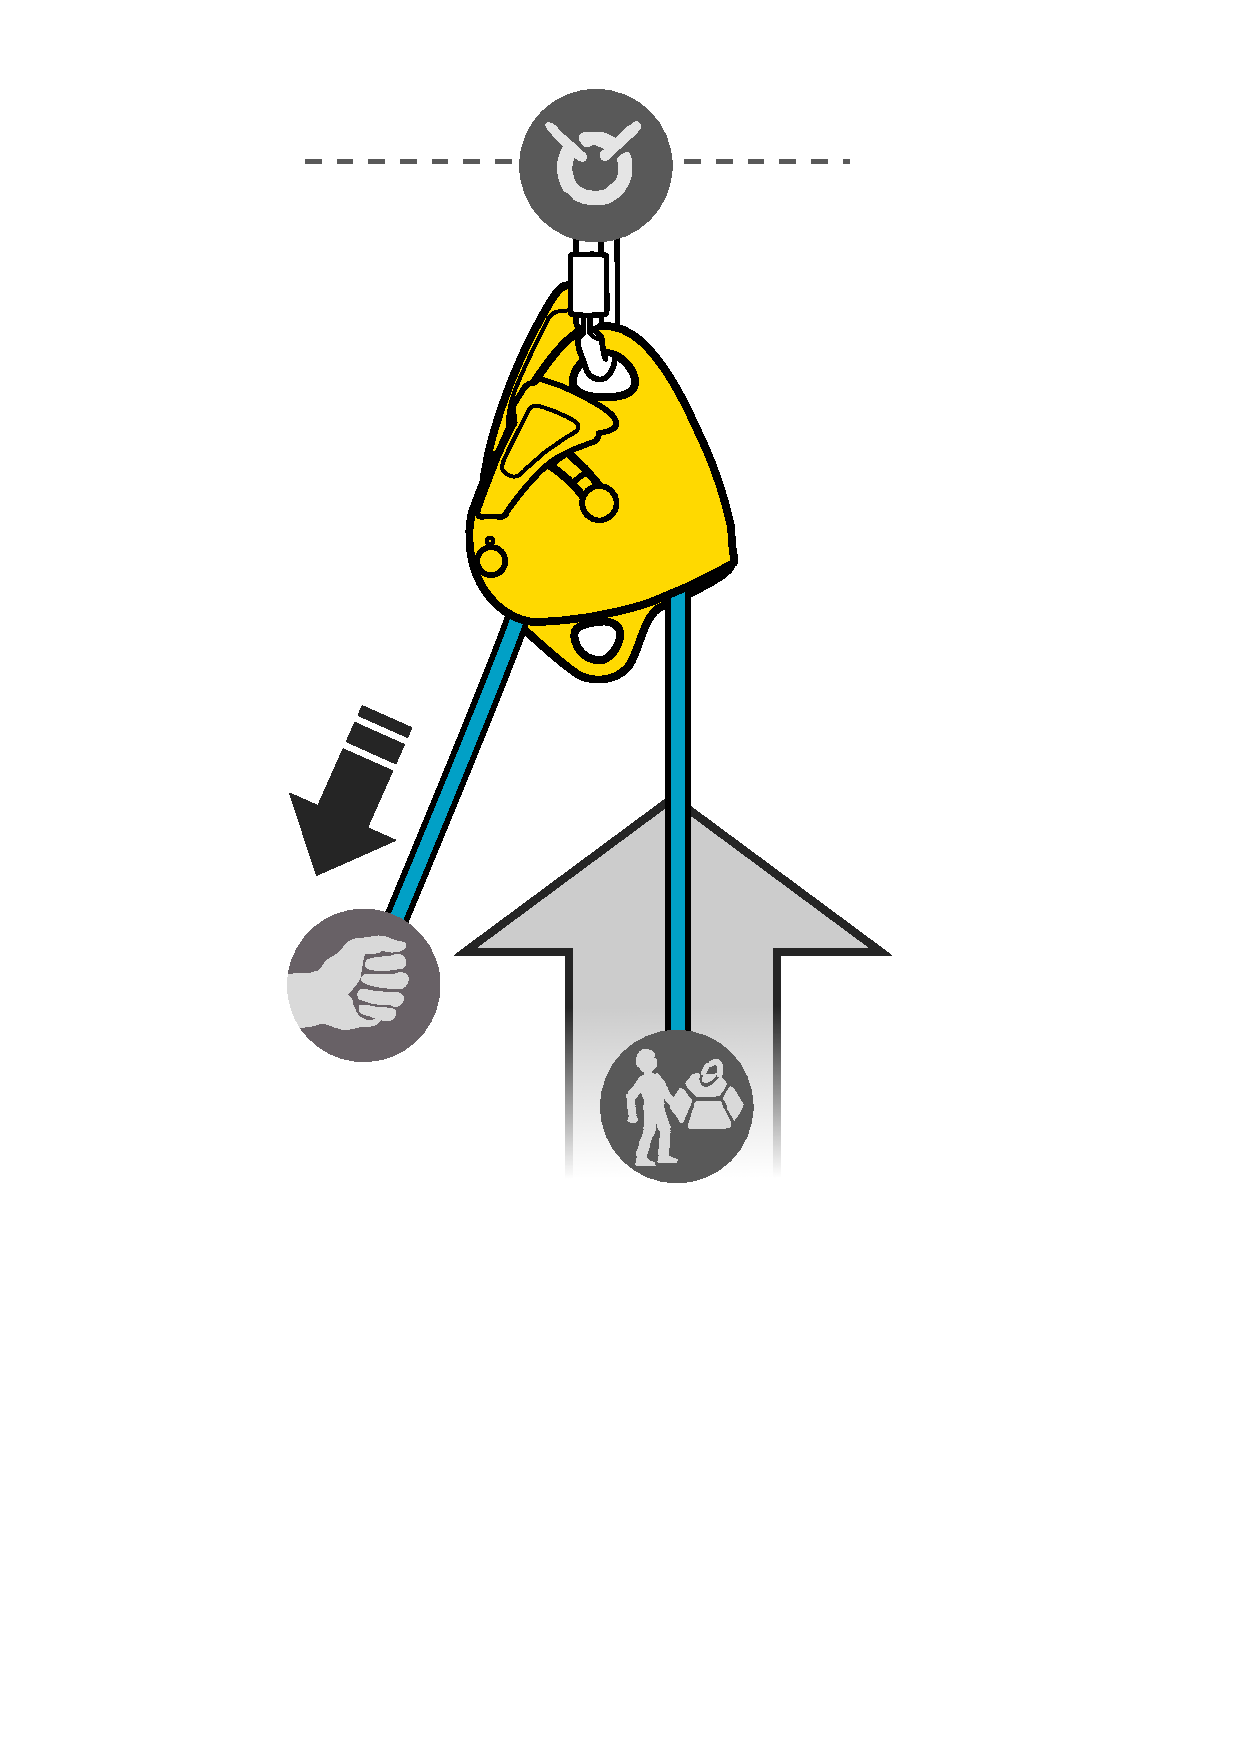
\includegraphics[width=5.0cm]{Figures/1_1/1_haul_system_1_1.pdf}}%
    \hfill % Seperation
    \subcaptionbox{Schéma kladkostroje\label{Obr:1:1_diagram}}{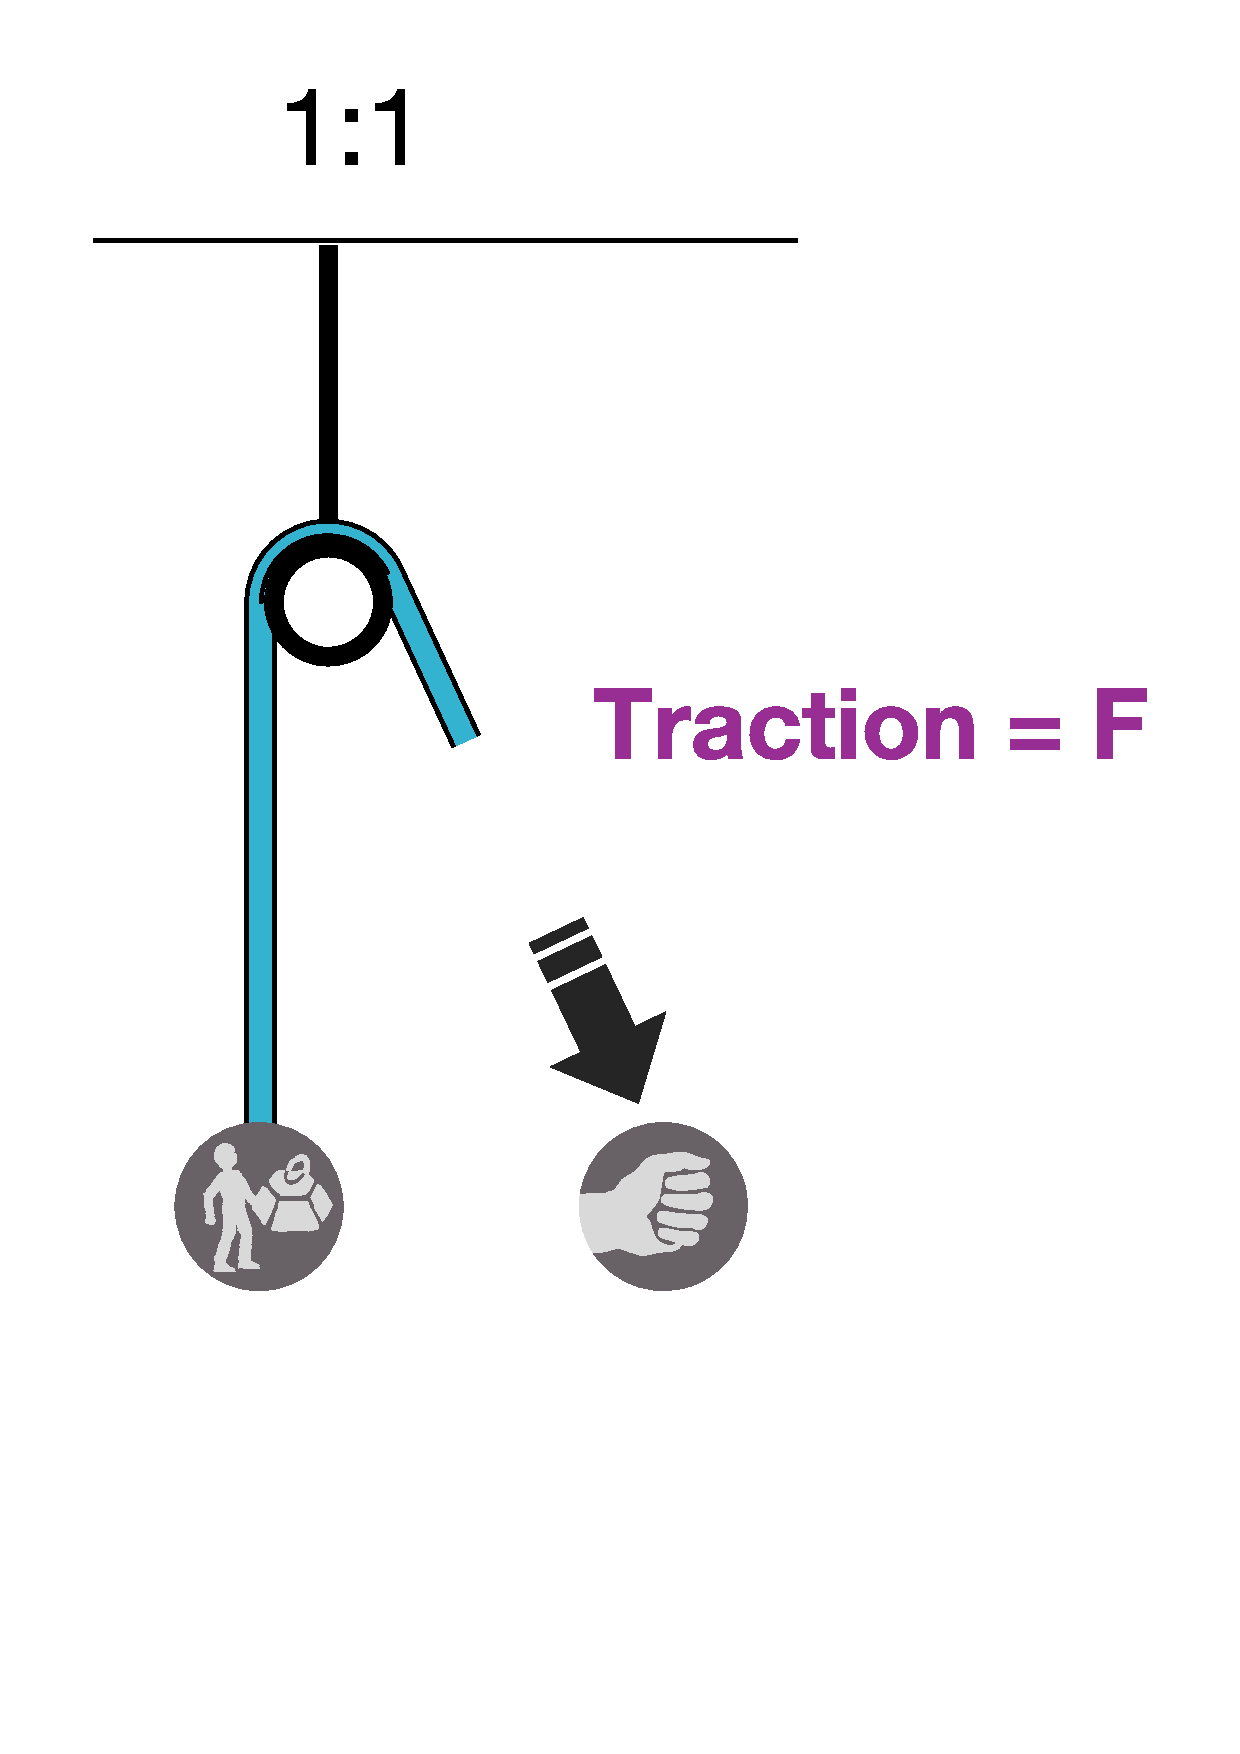
\includegraphics[width=5.0cm]{Figures/1_1/2_haul_system_1_1.pdf}}%
    \\ % Line break
    \subcaptionbox{Rozložení sil\label{Obr:1:1_forces_distribution}}{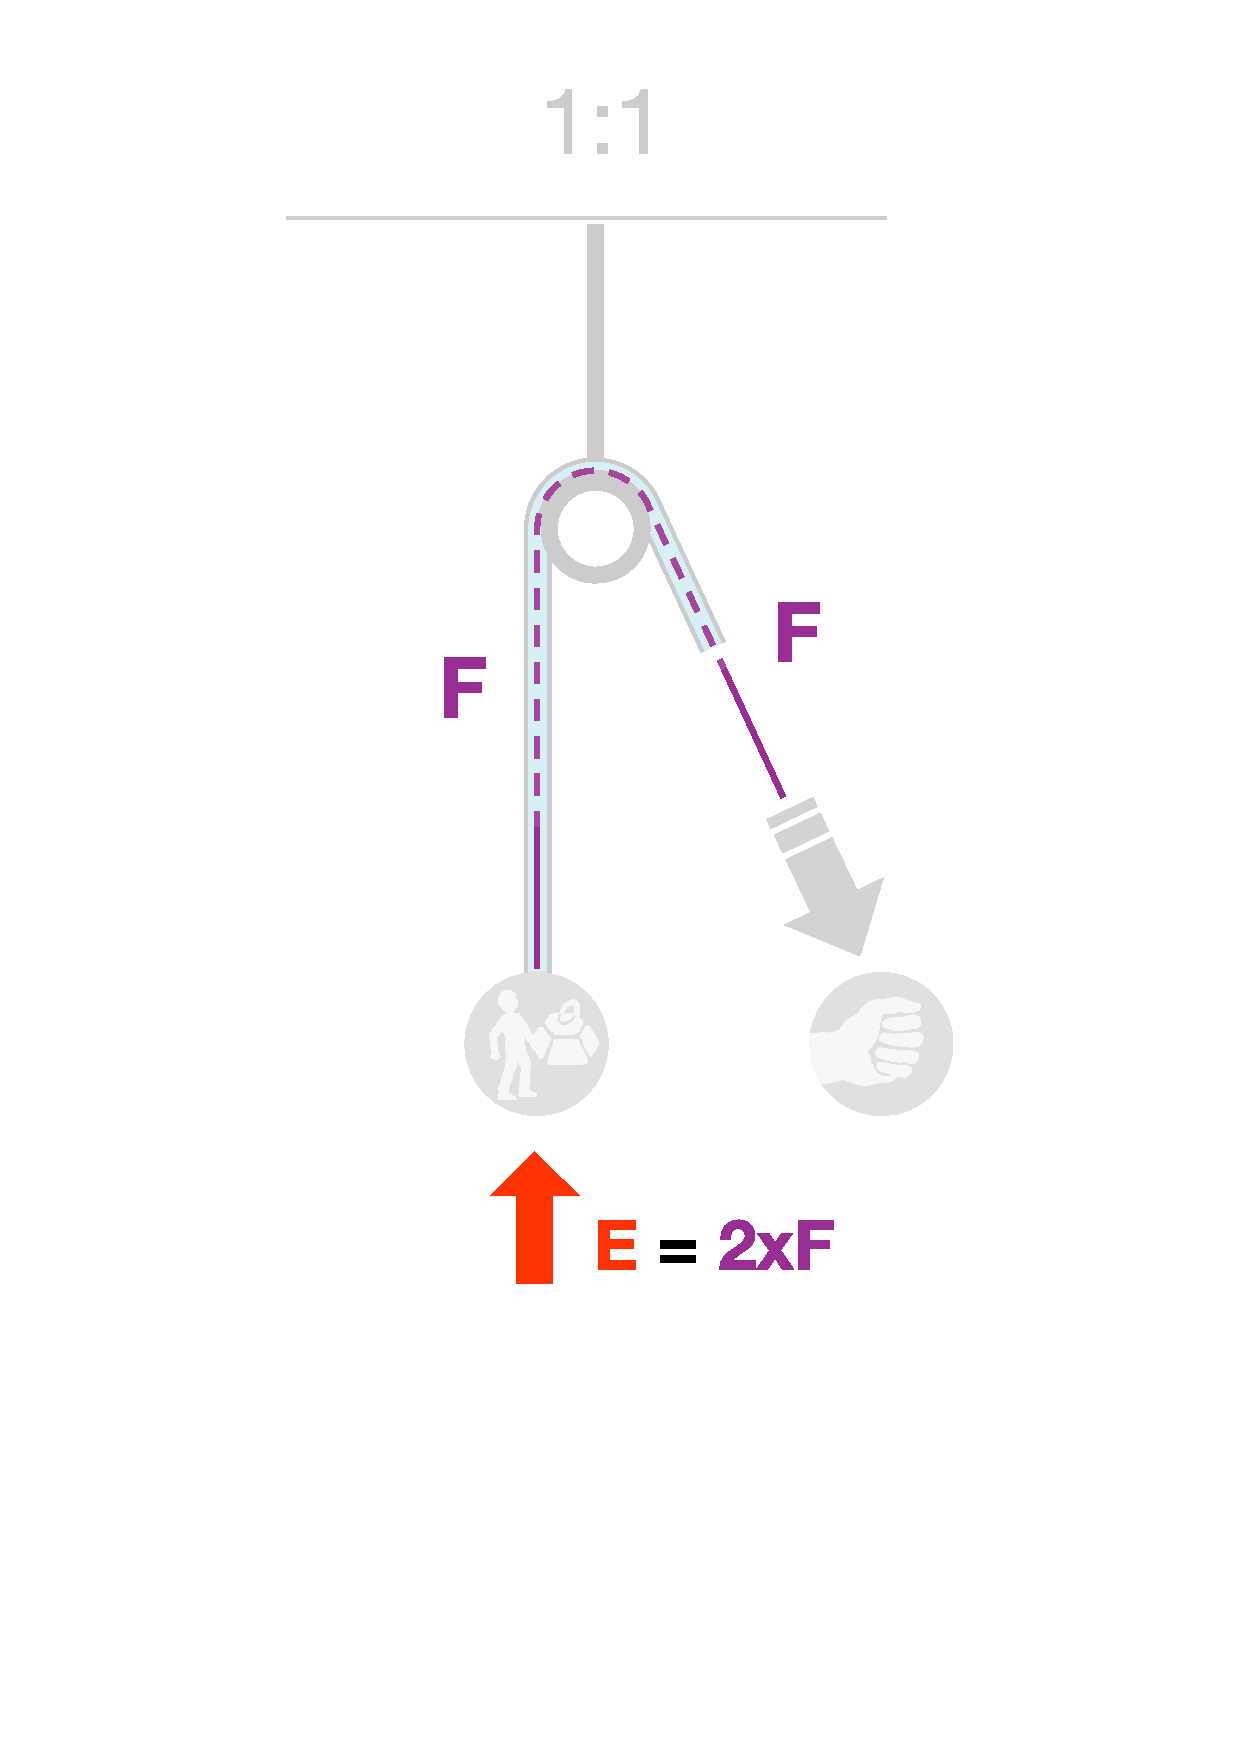
\includegraphics[width=5.0cm]{Figures/1_1/3_haul_system_1_1.pdf}}%
    \caption[Kladkostroj 1:1]{Kladkostroj 1:1 (schéma převzato ze zdroje \cite{Petzl_2022})}
    \label{Obr:1:1}
\end{figure}
%% -------------------------------------------------- %%

\newpage
\subsection{Systém 2:1}
%% -------------------------------------------------- %%
%% -------------------- Pictures --------------------- %%
%% -------------------------------------------------- %%
\begin{figure}[h]
    \centering
    \subcaptionbox{Sestrojení kladkostroje\label{Obr:2:1_Pulley_system}}{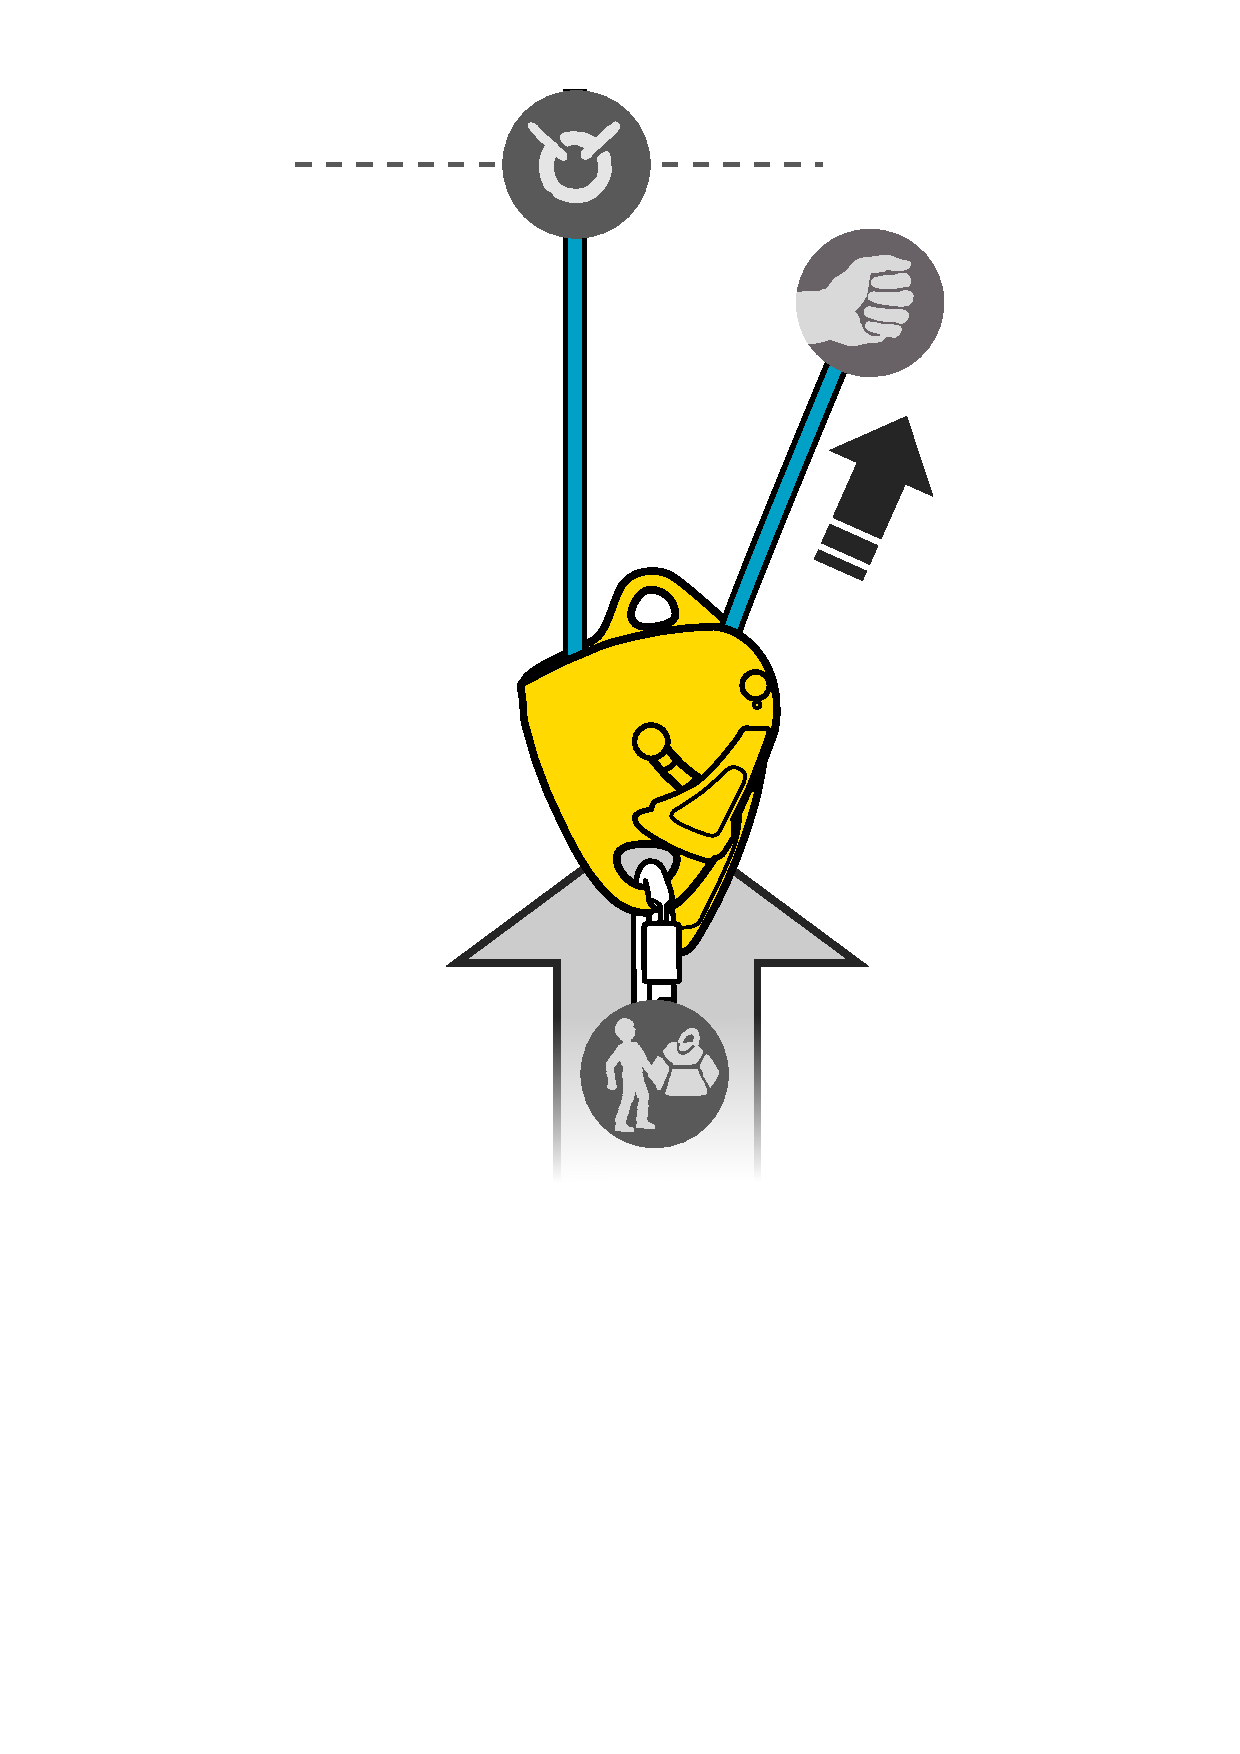
\includegraphics[width=5.0cm]{Figures/2_1/1_haul_system_2_1.pdf}}%
    \hfill % Seperation
    \subcaptionbox{Schéma kladkostroje\label{Obr:2:1_diagram}}{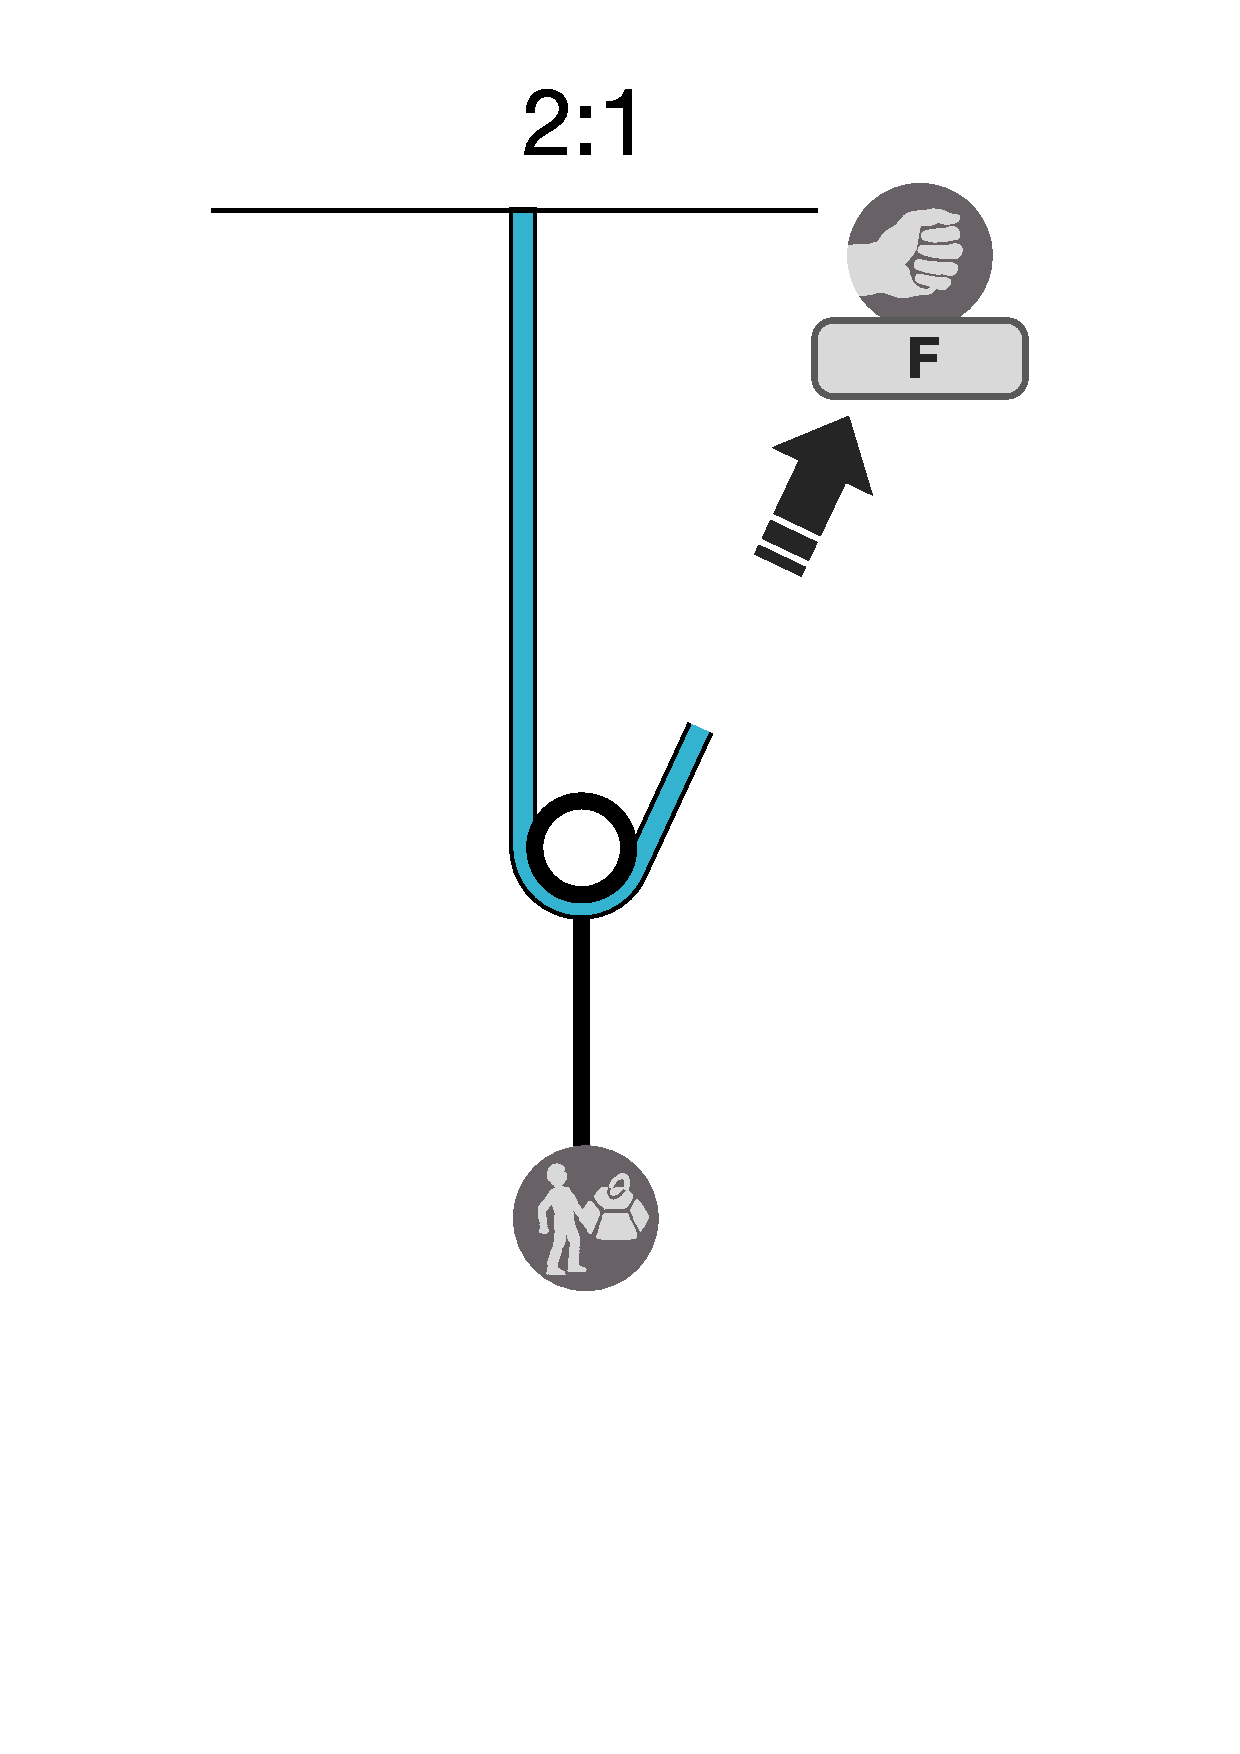
\includegraphics[width=5.0cm]{Figures/2_1/2_haul_system_2_1.pdf}}%
    \\ % Line break
    \subcaptionbox{Rozložení sil\label{Obr:2:1_forces_distribution}}{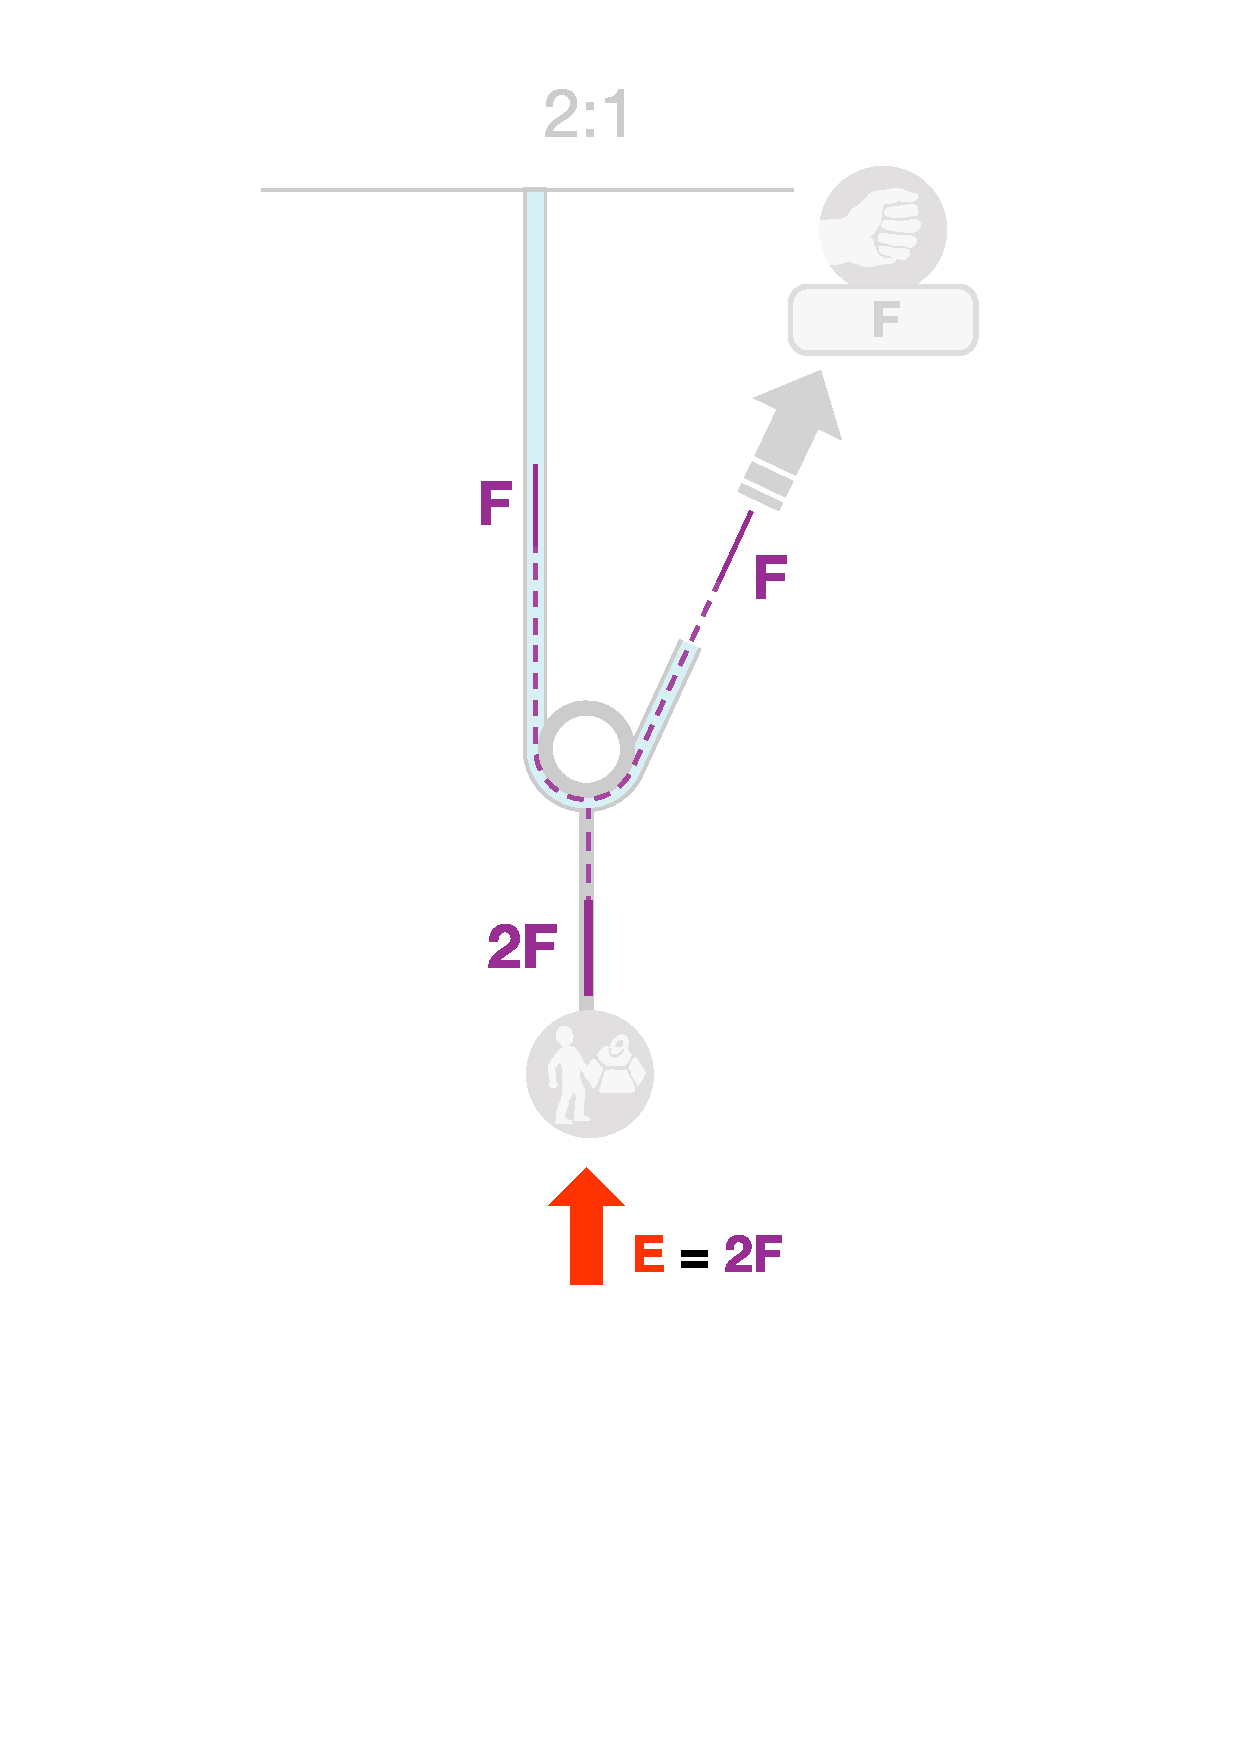
\includegraphics[width=5.0cm]{Figures/2_1/3_haul_system_2_1.pdf}}%
    \caption[Kladkostroj 2:1]{Kladkostroj 2:1 (schéma převzato ze zdroje \cite{Petzl_2022})}
    \label{Obr:2:1}
\end{figure}
%% -------------------------------------------------- %%

\newpage
\subsection{Systém 3:1}
%% -------------------------------------------------- %%
%% -------------------- Pictures --------------------- %%
%% -------------------------------------------------- %%
\begin{figure}[h]
    \centering
    \subcaptionbox{Sestrojení kladkostroje\label{Obr:3:1_Pulley_system}}{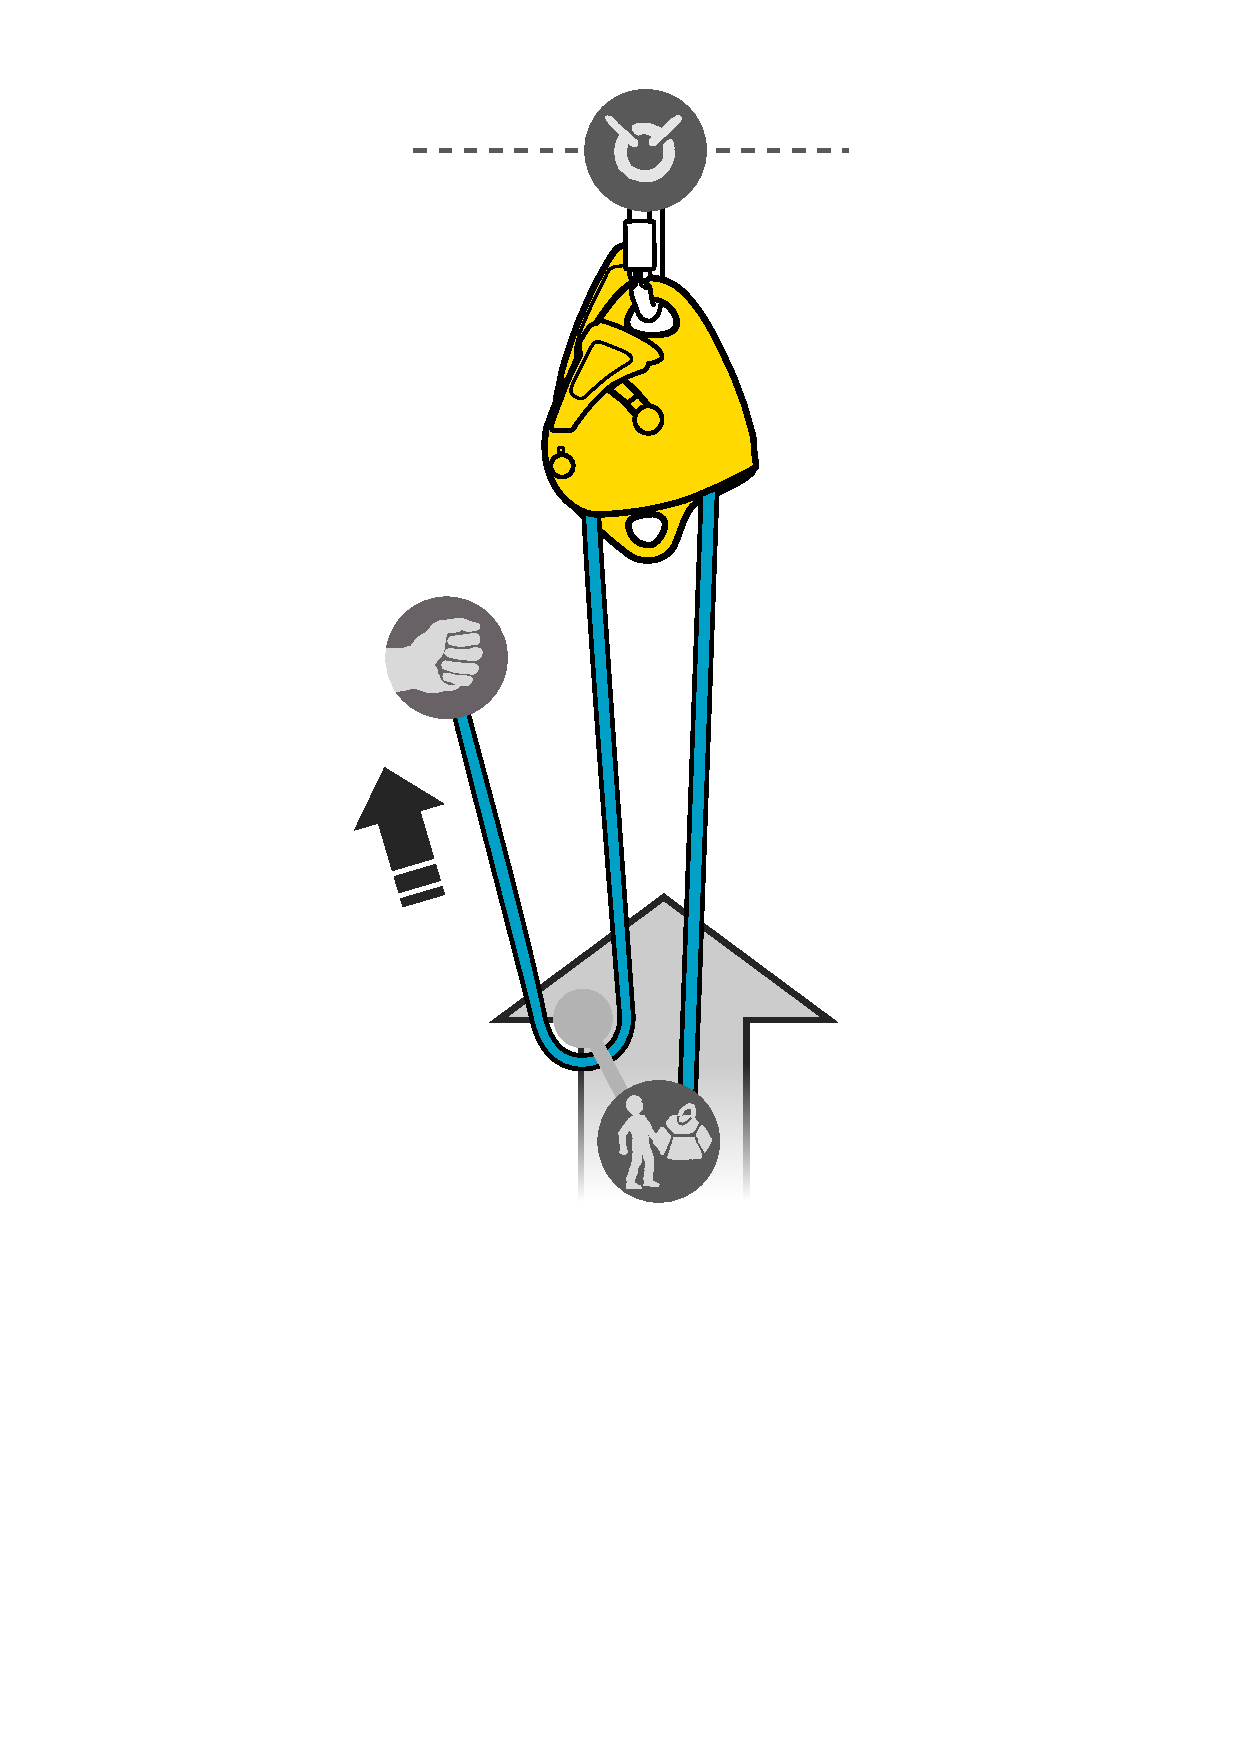
\includegraphics[width=4.0cm]{Figures/3_1/1_haul_system_3_1.pdf}}%
    \hfill % Seperation
    \subcaptionbox{Zobrazení sestrojeného kladkostroje\label{Obr:3:1_Figure_pulley_system}}{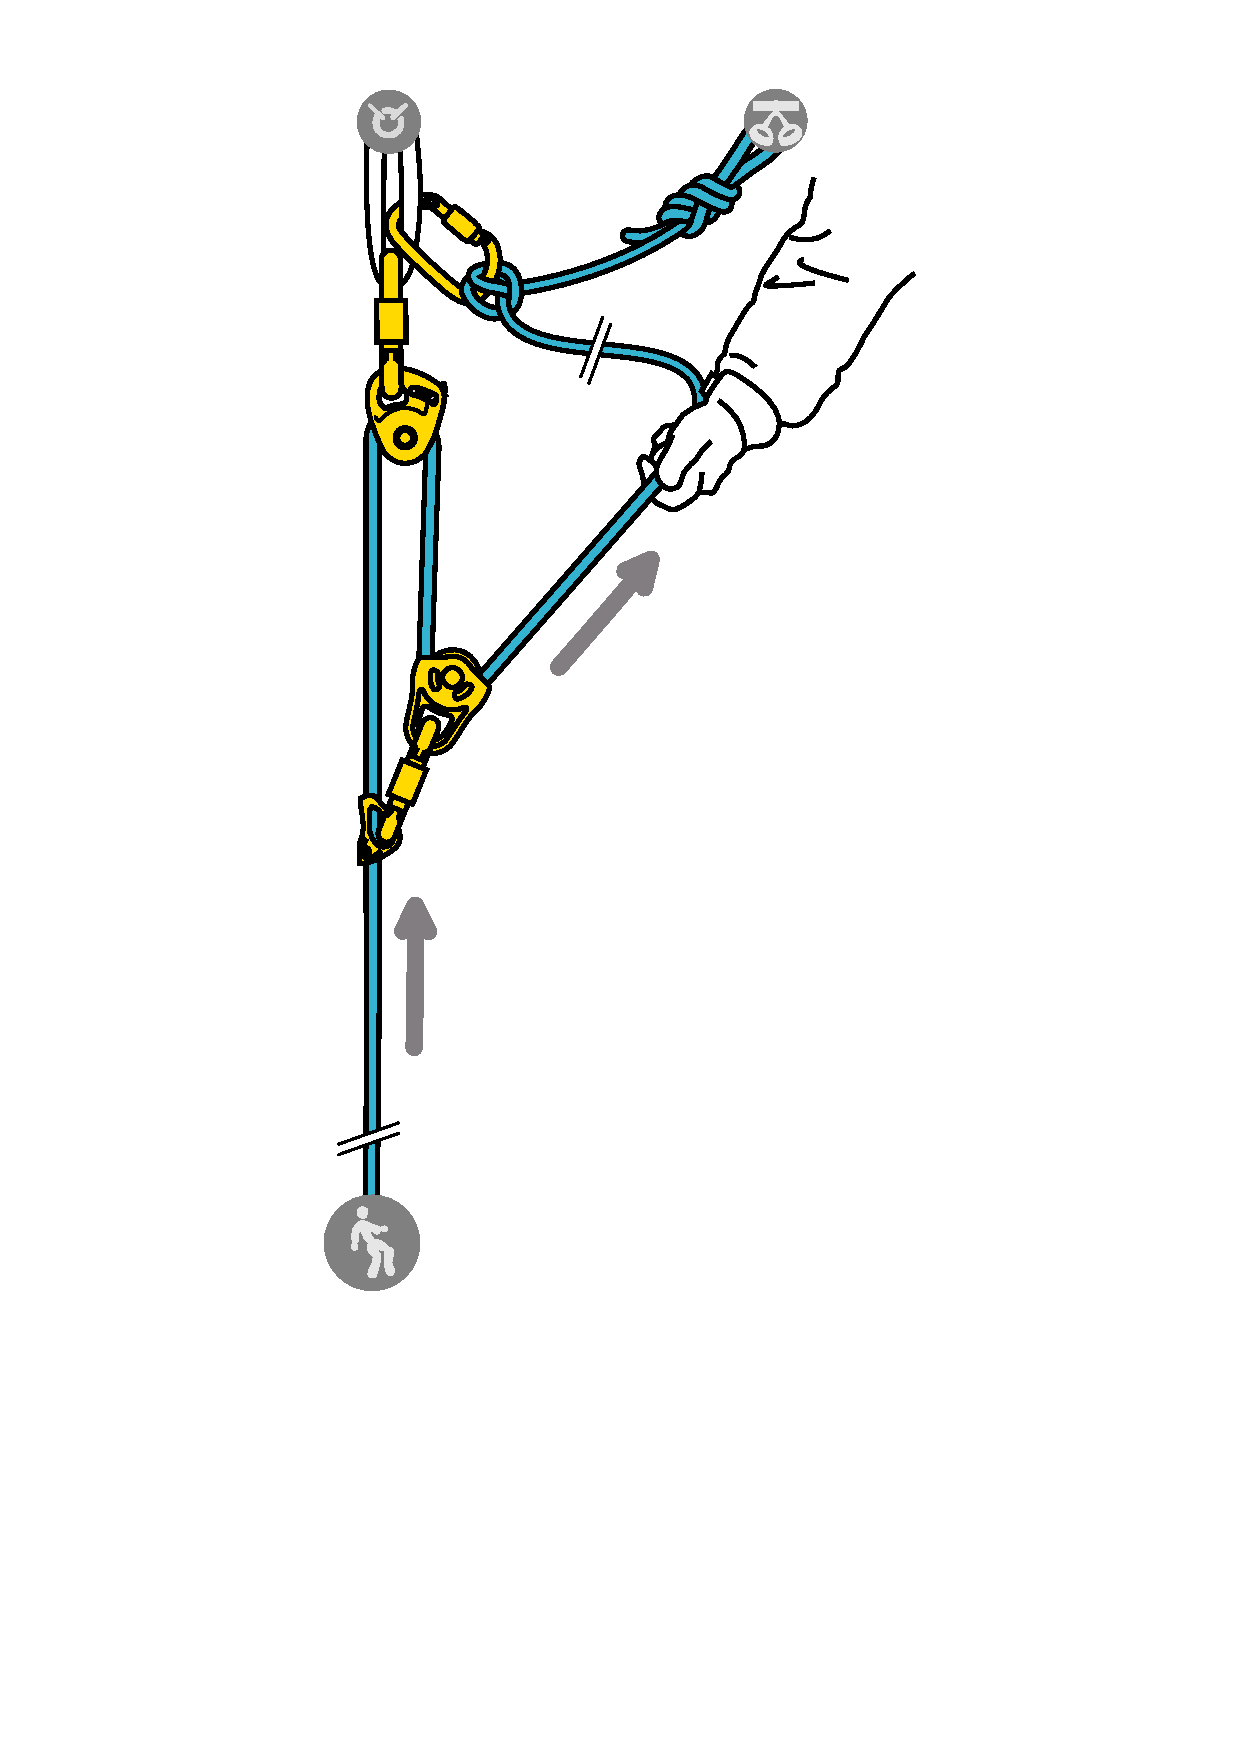
\includegraphics[width=5.0cm]{Figures/3_1/2_haul_system_3_1.pdf}}%
    \\ % Line break
    \subcaptionbox{Schéma kladkostroje\label{Obr:3:1_diagram}}{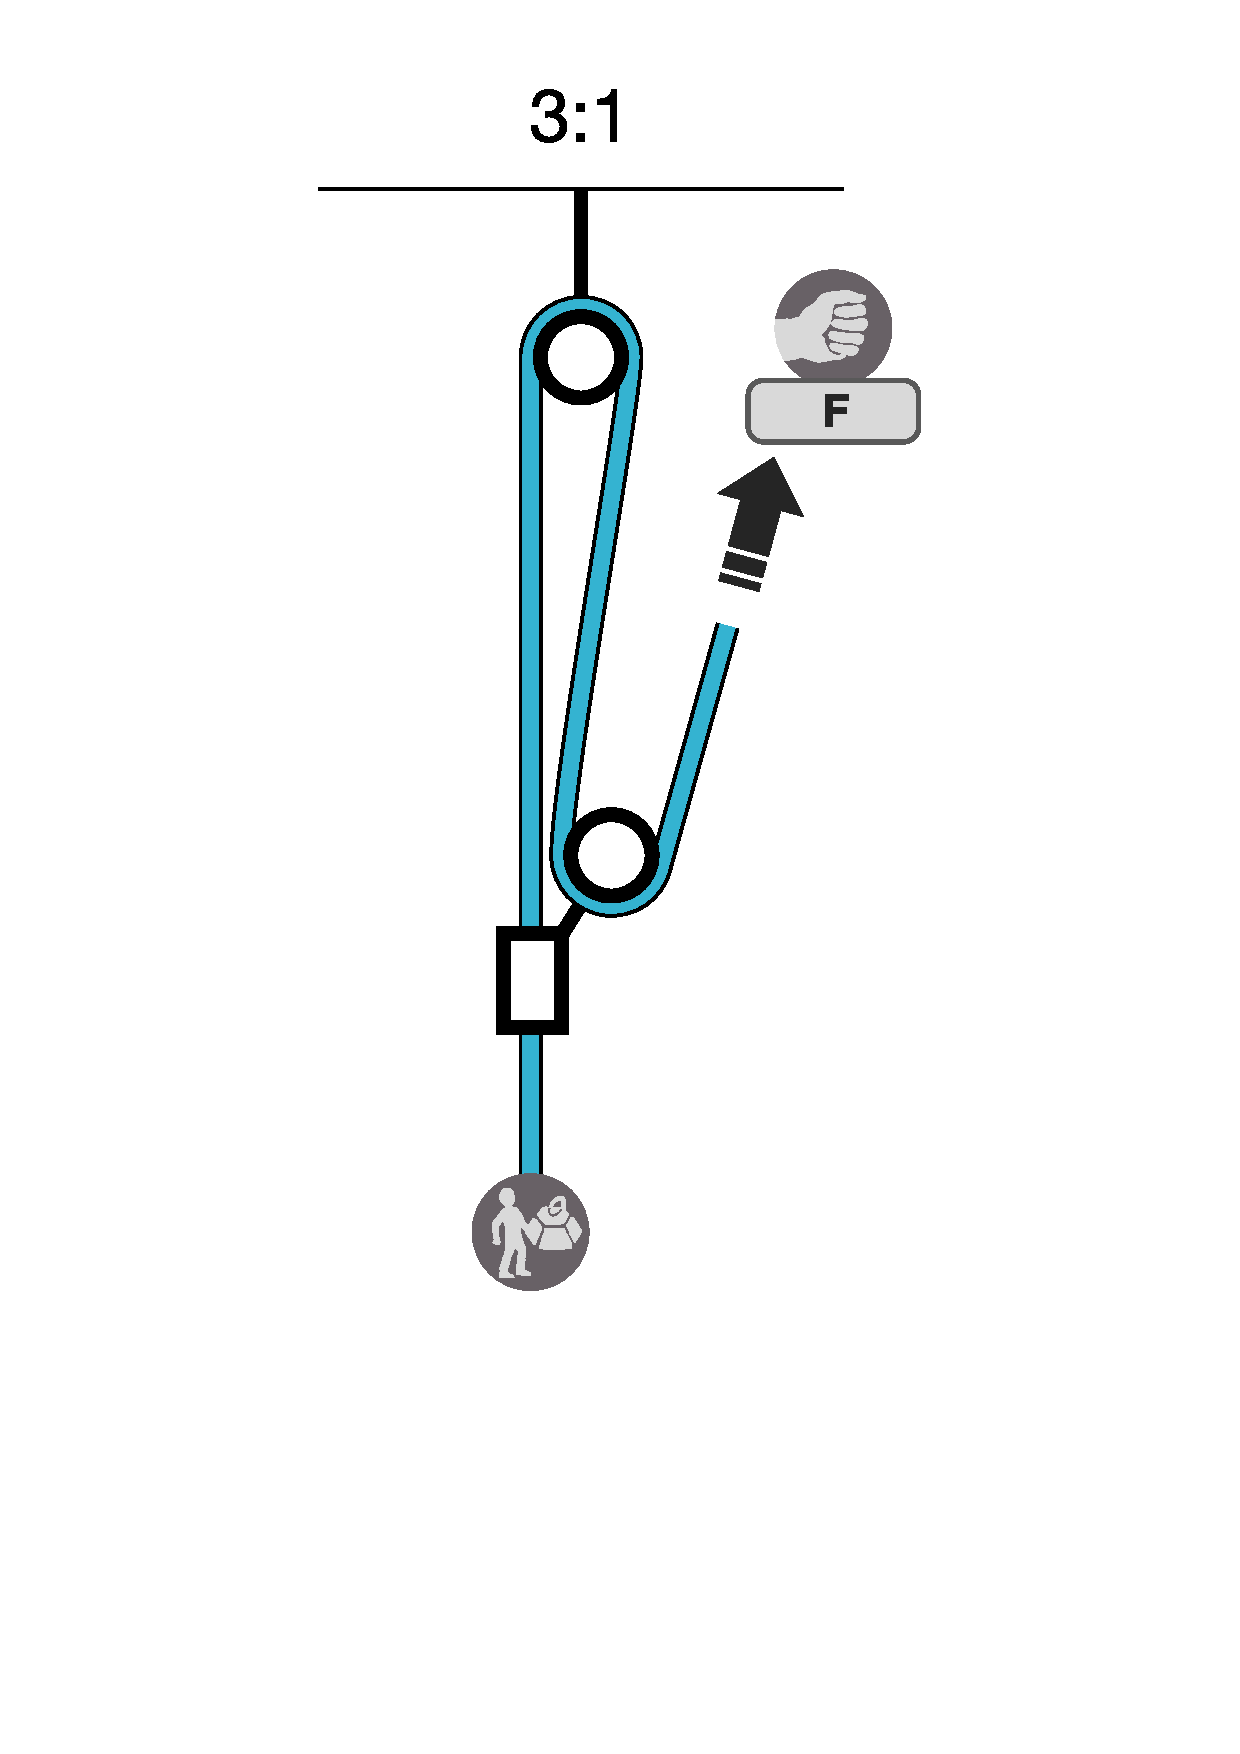
\includegraphics[width=4.0cm]{Figures/3_1/3_haul_system_3_1.pdf}}%
    \hfill % Seperation
    \subcaptionbox{Rozložení sil\label{Obr:3:1_forces_distribution}}{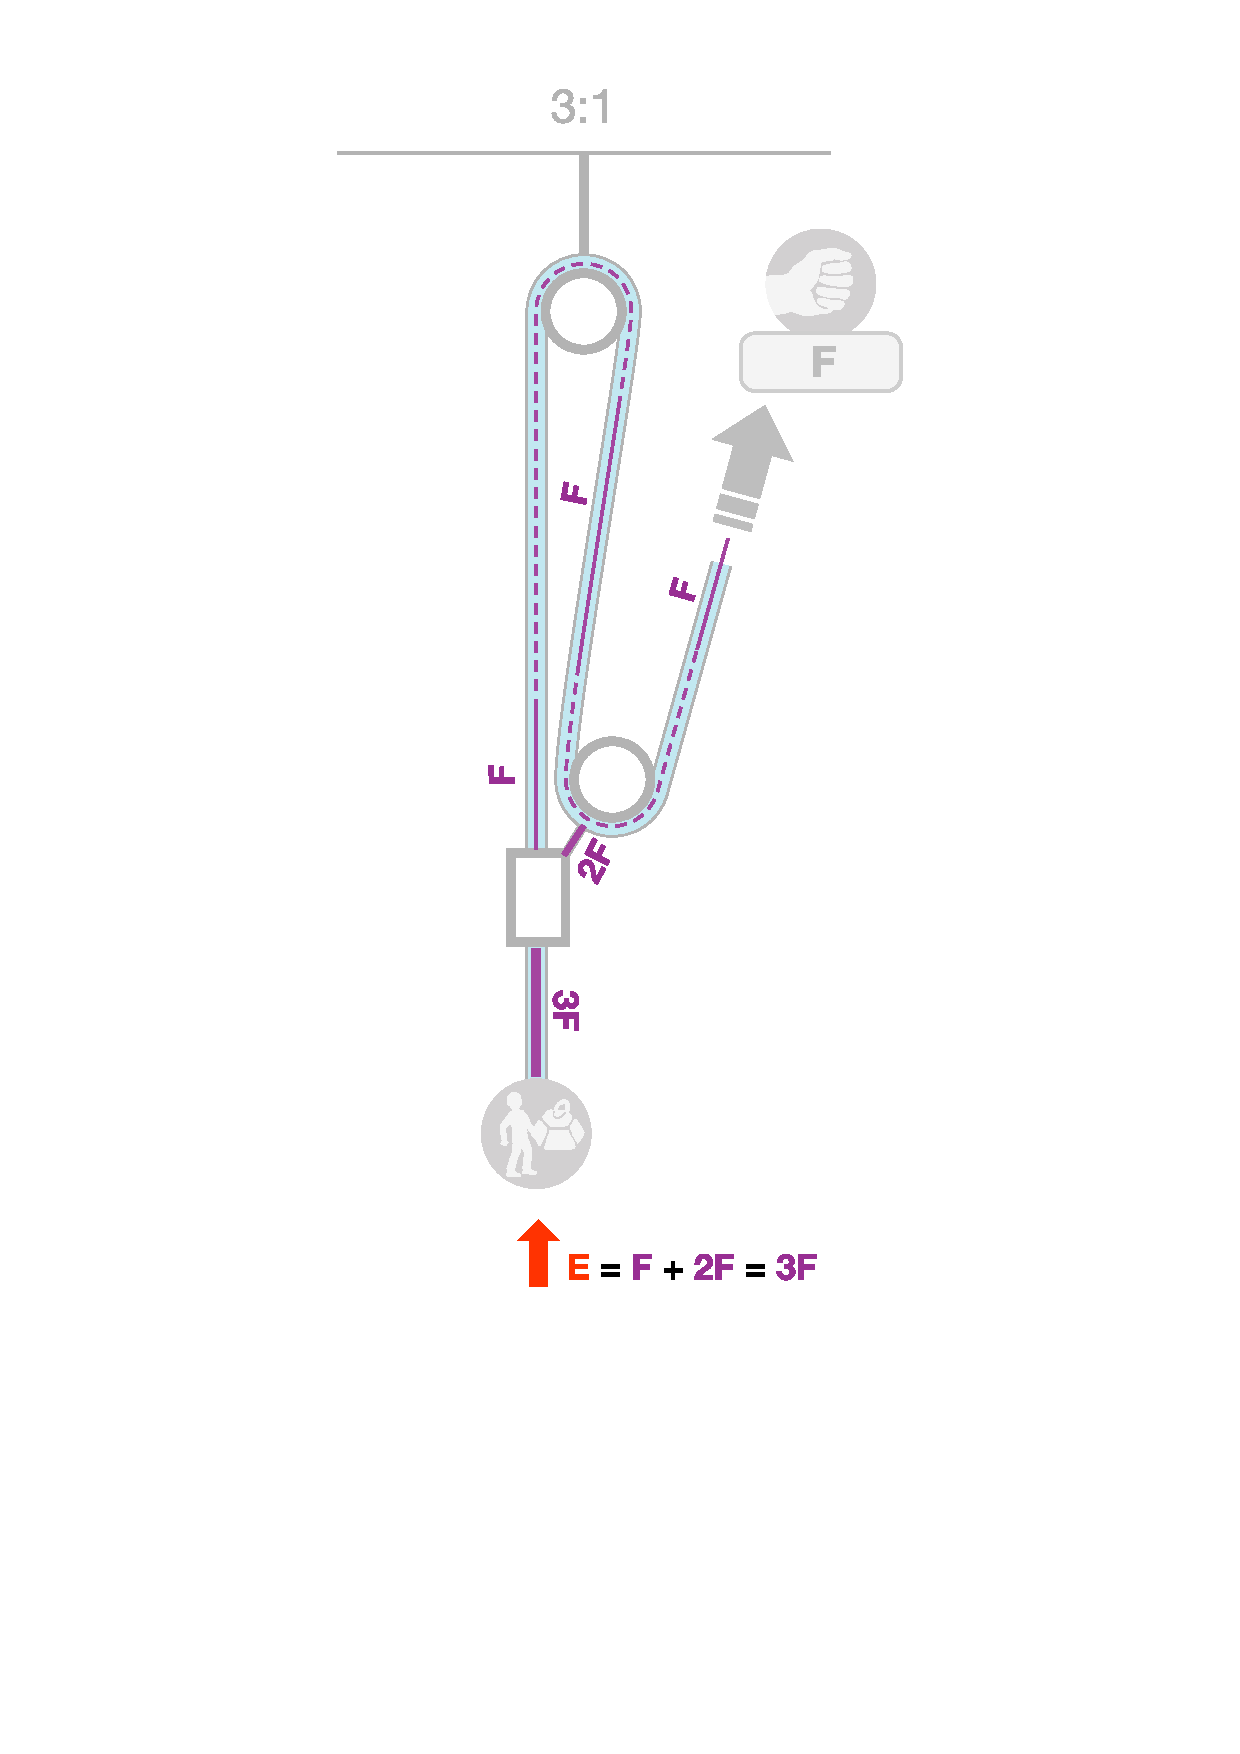
\includegraphics[width=4.0cm]{Figures/3_1/4_haul_system_3_1.pdf}}%
    \caption[Kladkostroj 3:1]{Kladkostroj 3:1 (schéma převzato ze zdroje \cite{Petzl_2022})}
    \label{Obr:3:1}
\end{figure}
%% -------------------------------------------------- %%

\newpage
\subsection{Systém 4:1}
%% -------------------------------------------------- %%
%% -------------------- Pictures --------------------- %%
%% -------------------------------------------------- %%
\begin{figure}[h]
    \centering
    \subcaptionbox{Sestrojení kladkostroje\label{Obr:4:1_Pulley_system}}{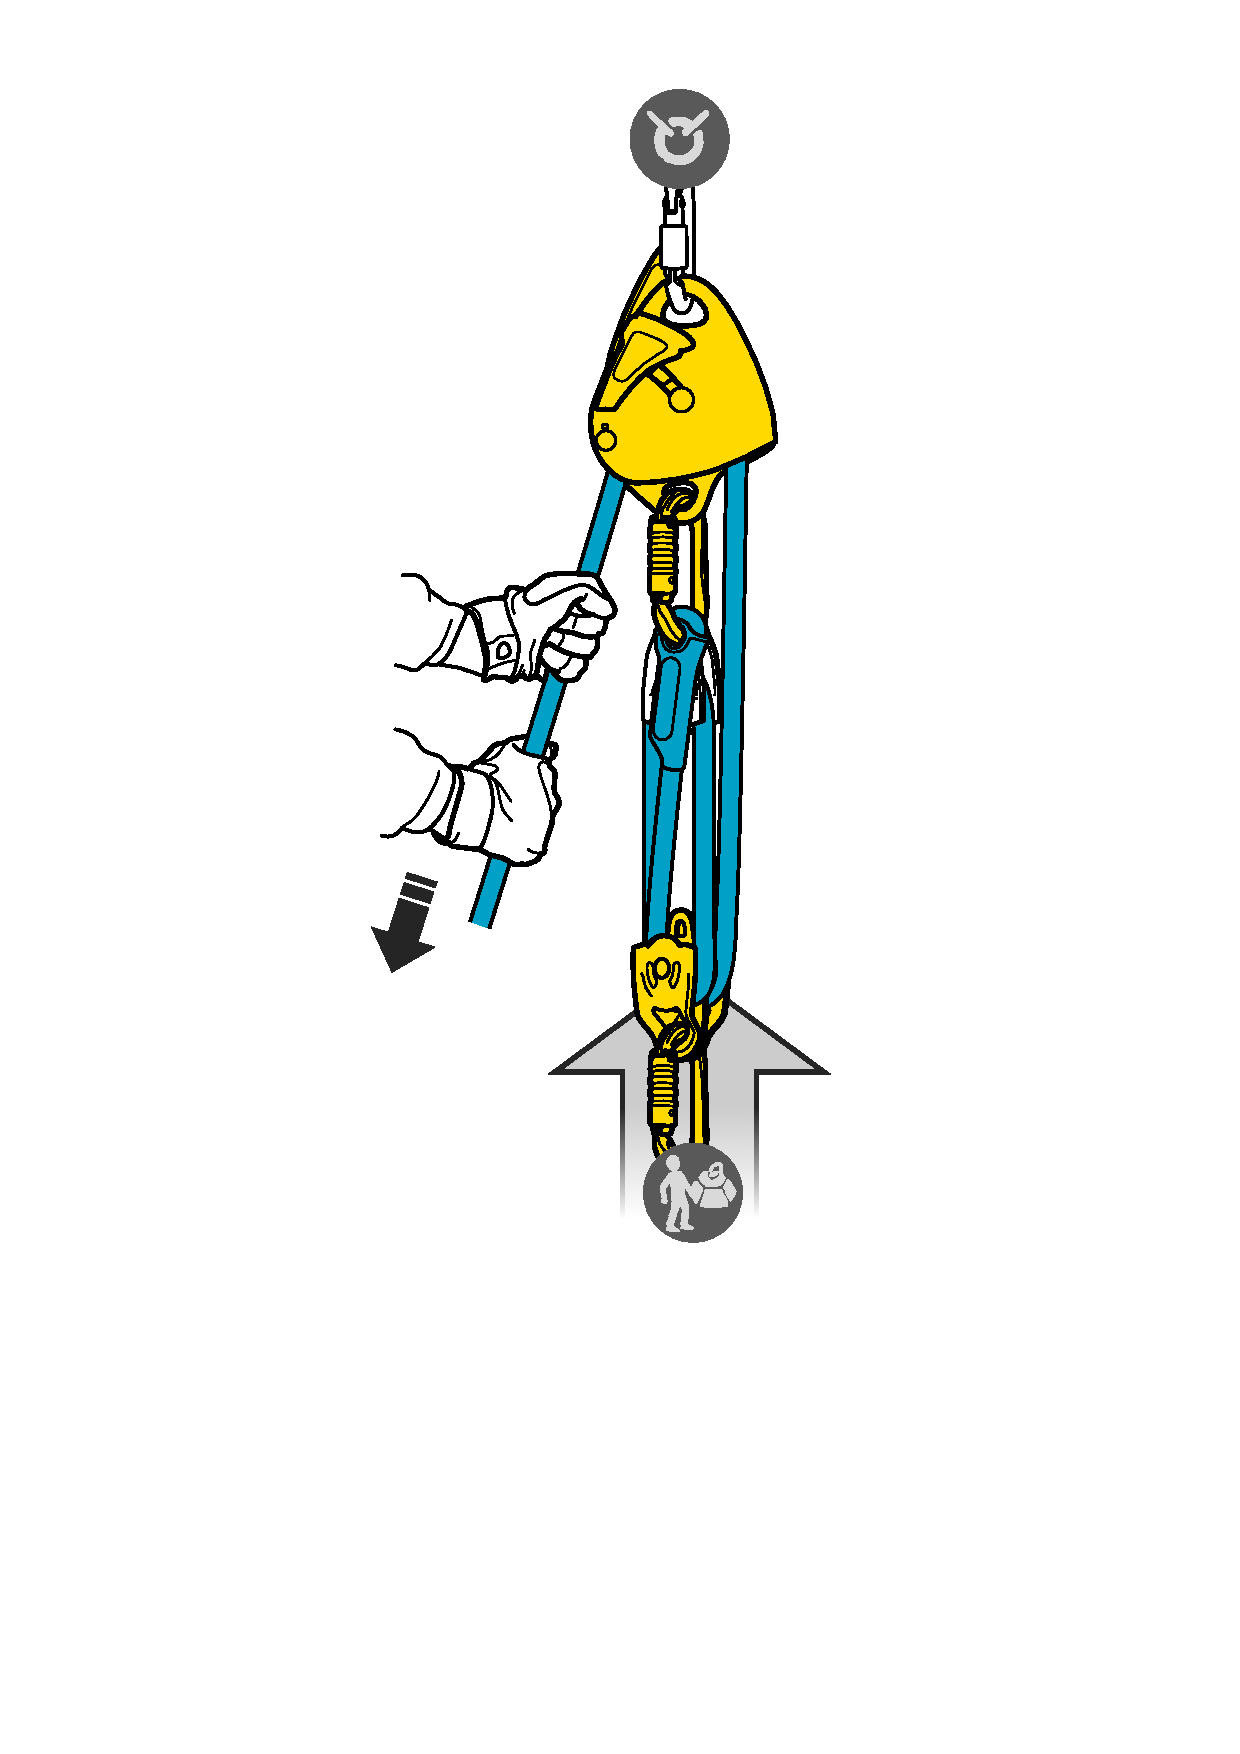
\includegraphics[width=4.0cm]{Figures/4_1/1_haul_system_4_1.pdf}}%
    \hfill % Seperation
    \subcaptionbox{Zobrazení sestrojeného kladkostroje\label{Obr:4:1_Figure_pulley_system}}{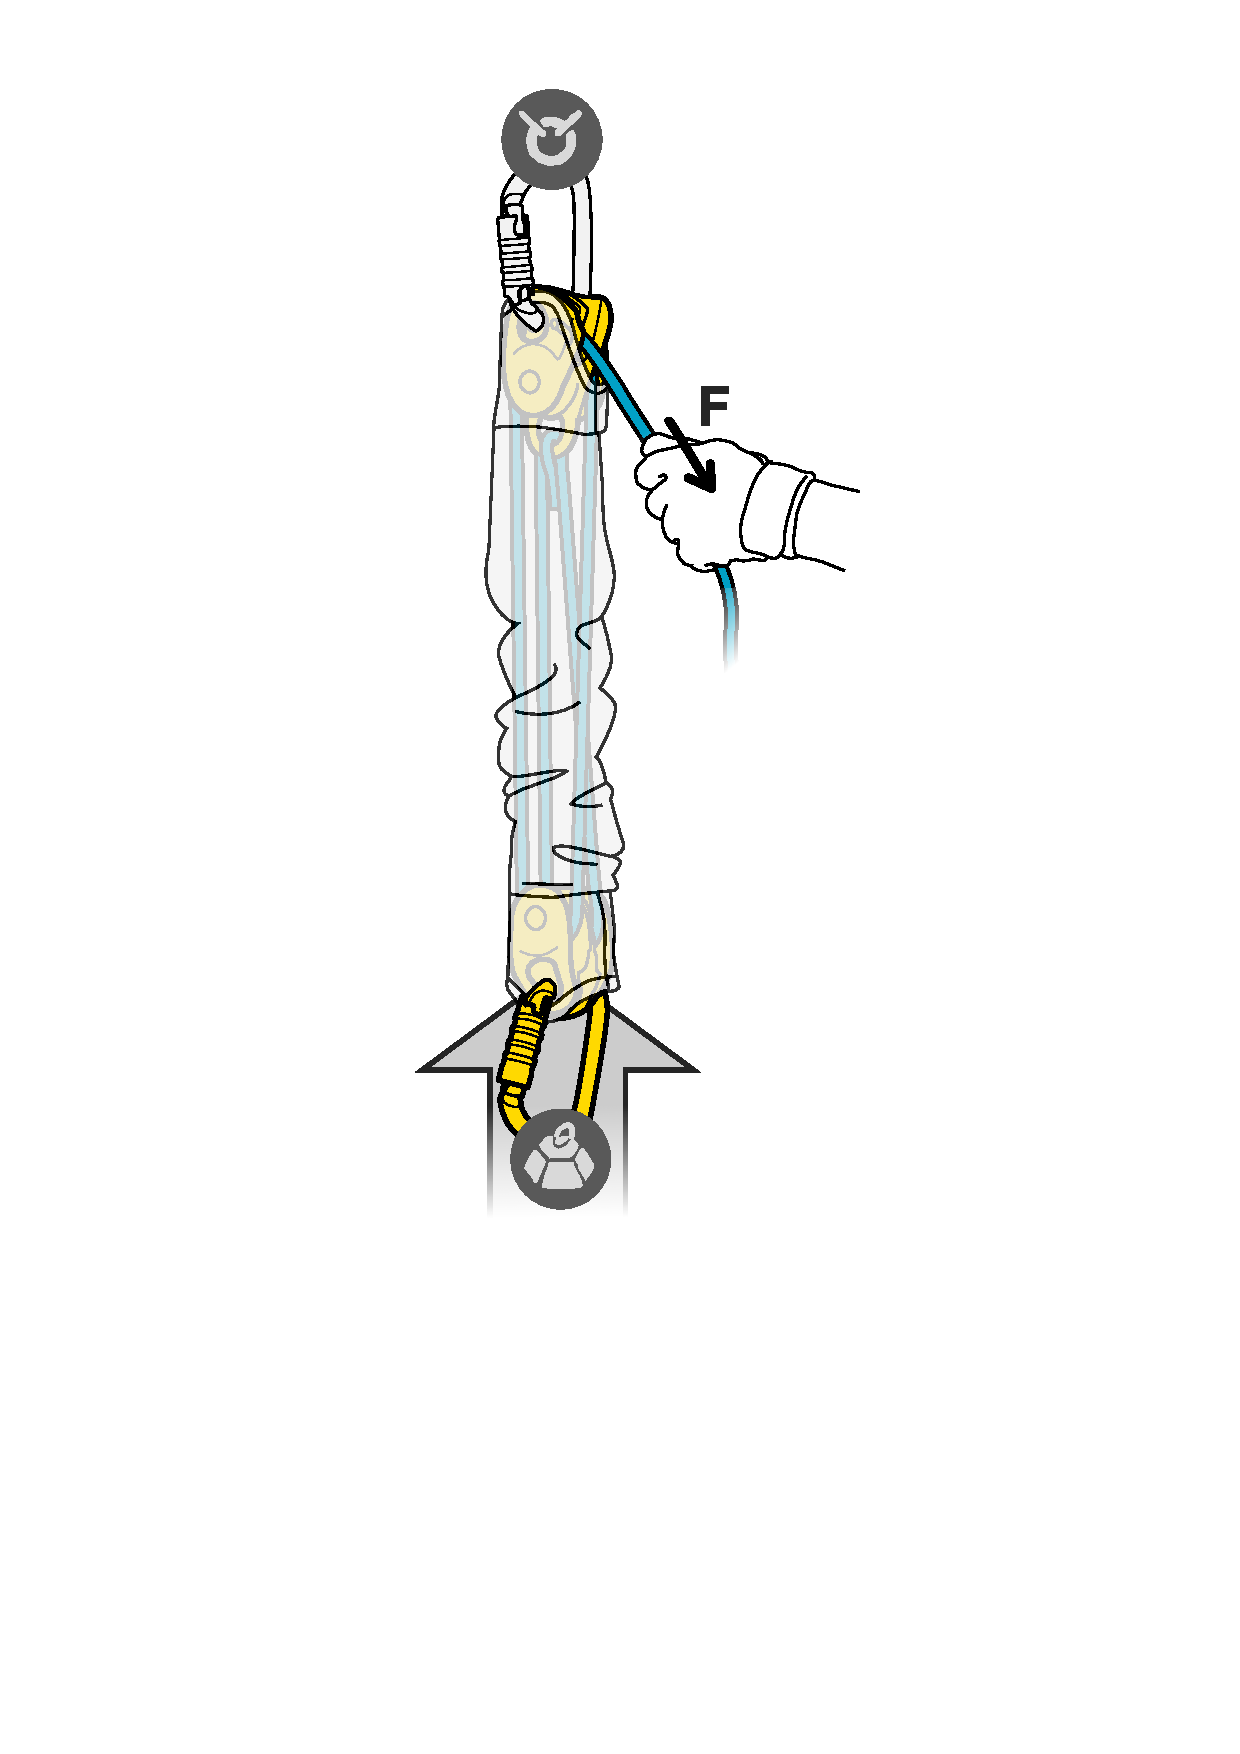
\includegraphics[width=4.0cm]{Figures/4_1/2_haul_system_4_1.pdf}}%
    \\ % Line break
    \subcaptionbox{Schéma kladkostroje\label{Obr:4:1_diagram}}{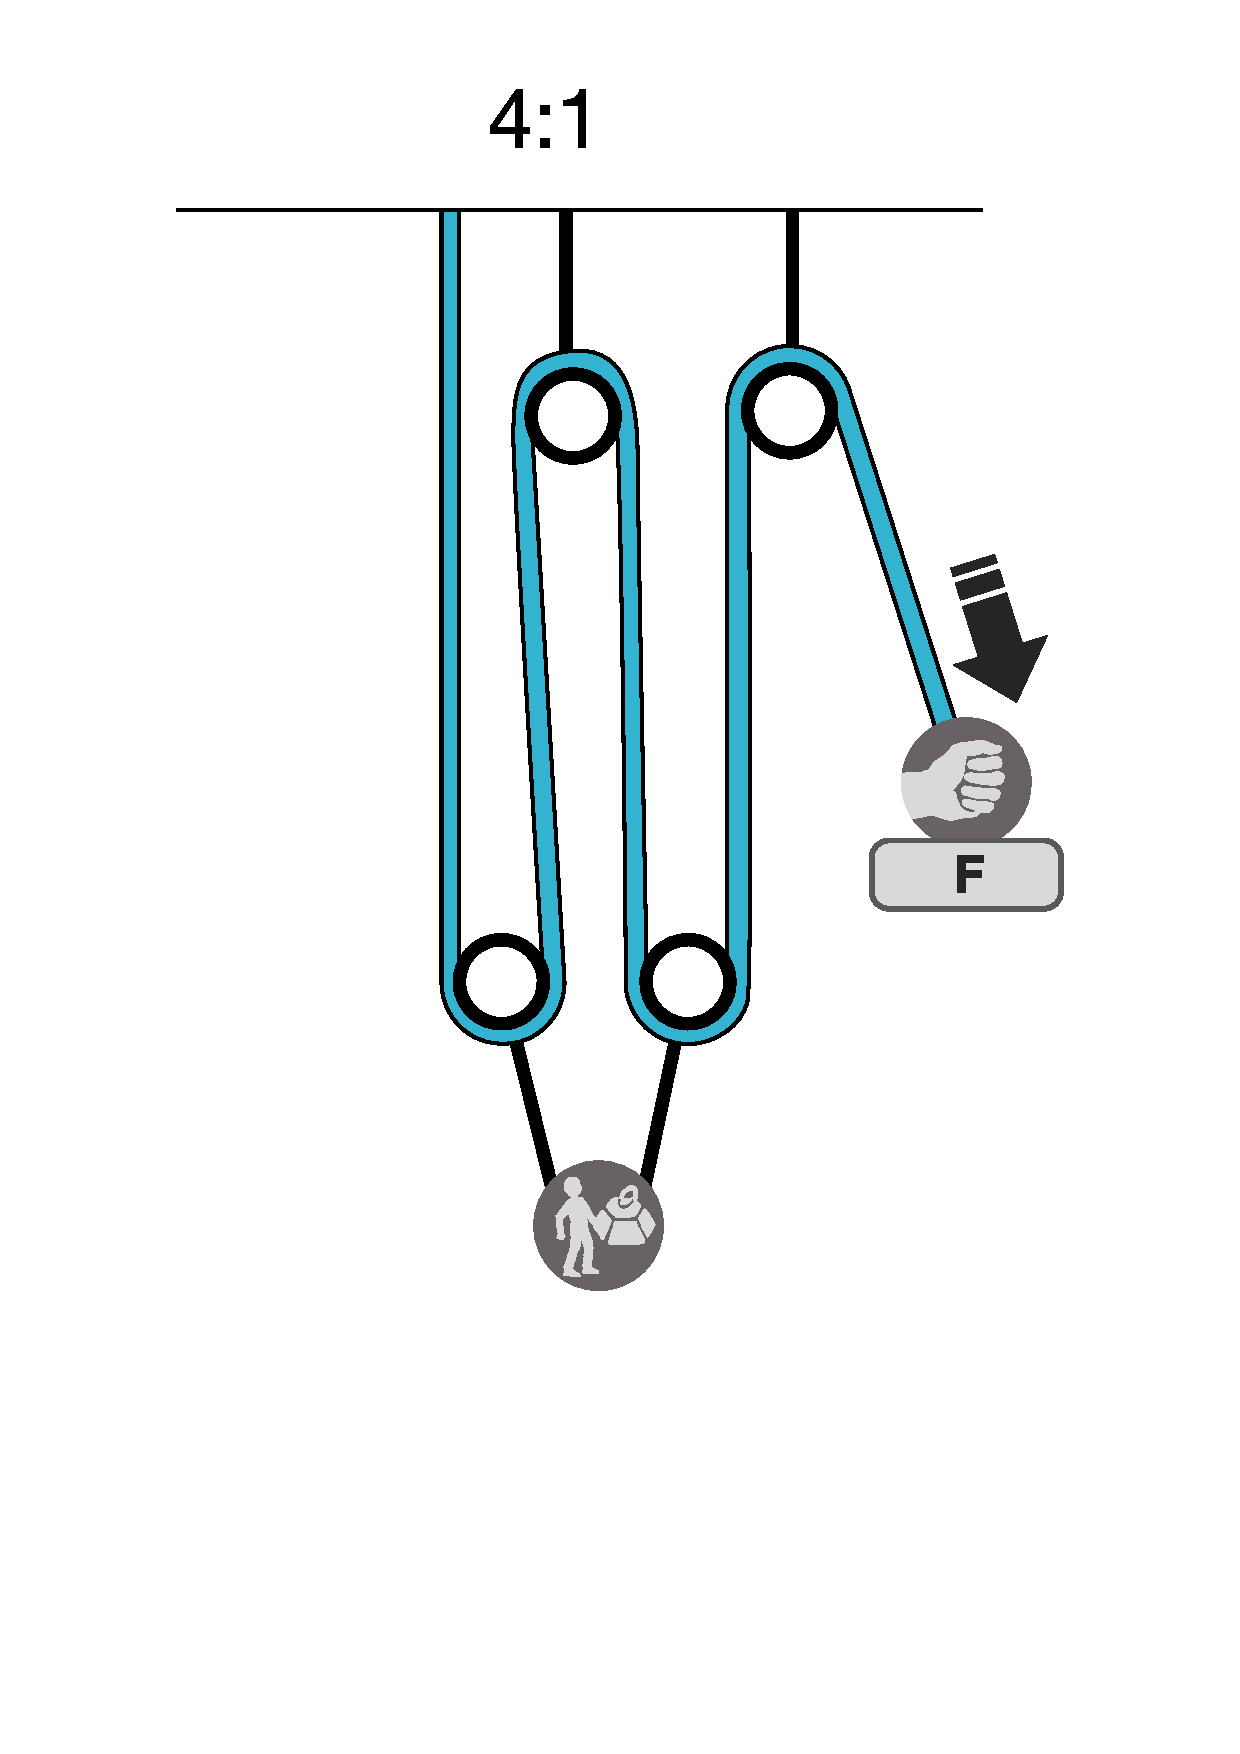
\includegraphics[width=4.0cm]{Figures/4_1/3_haul_system_4_1.pdf}}%
    \hfill % Seperation
    \subcaptionbox{Rozložení sil\label{Obr:4:1_forces_distribution}}{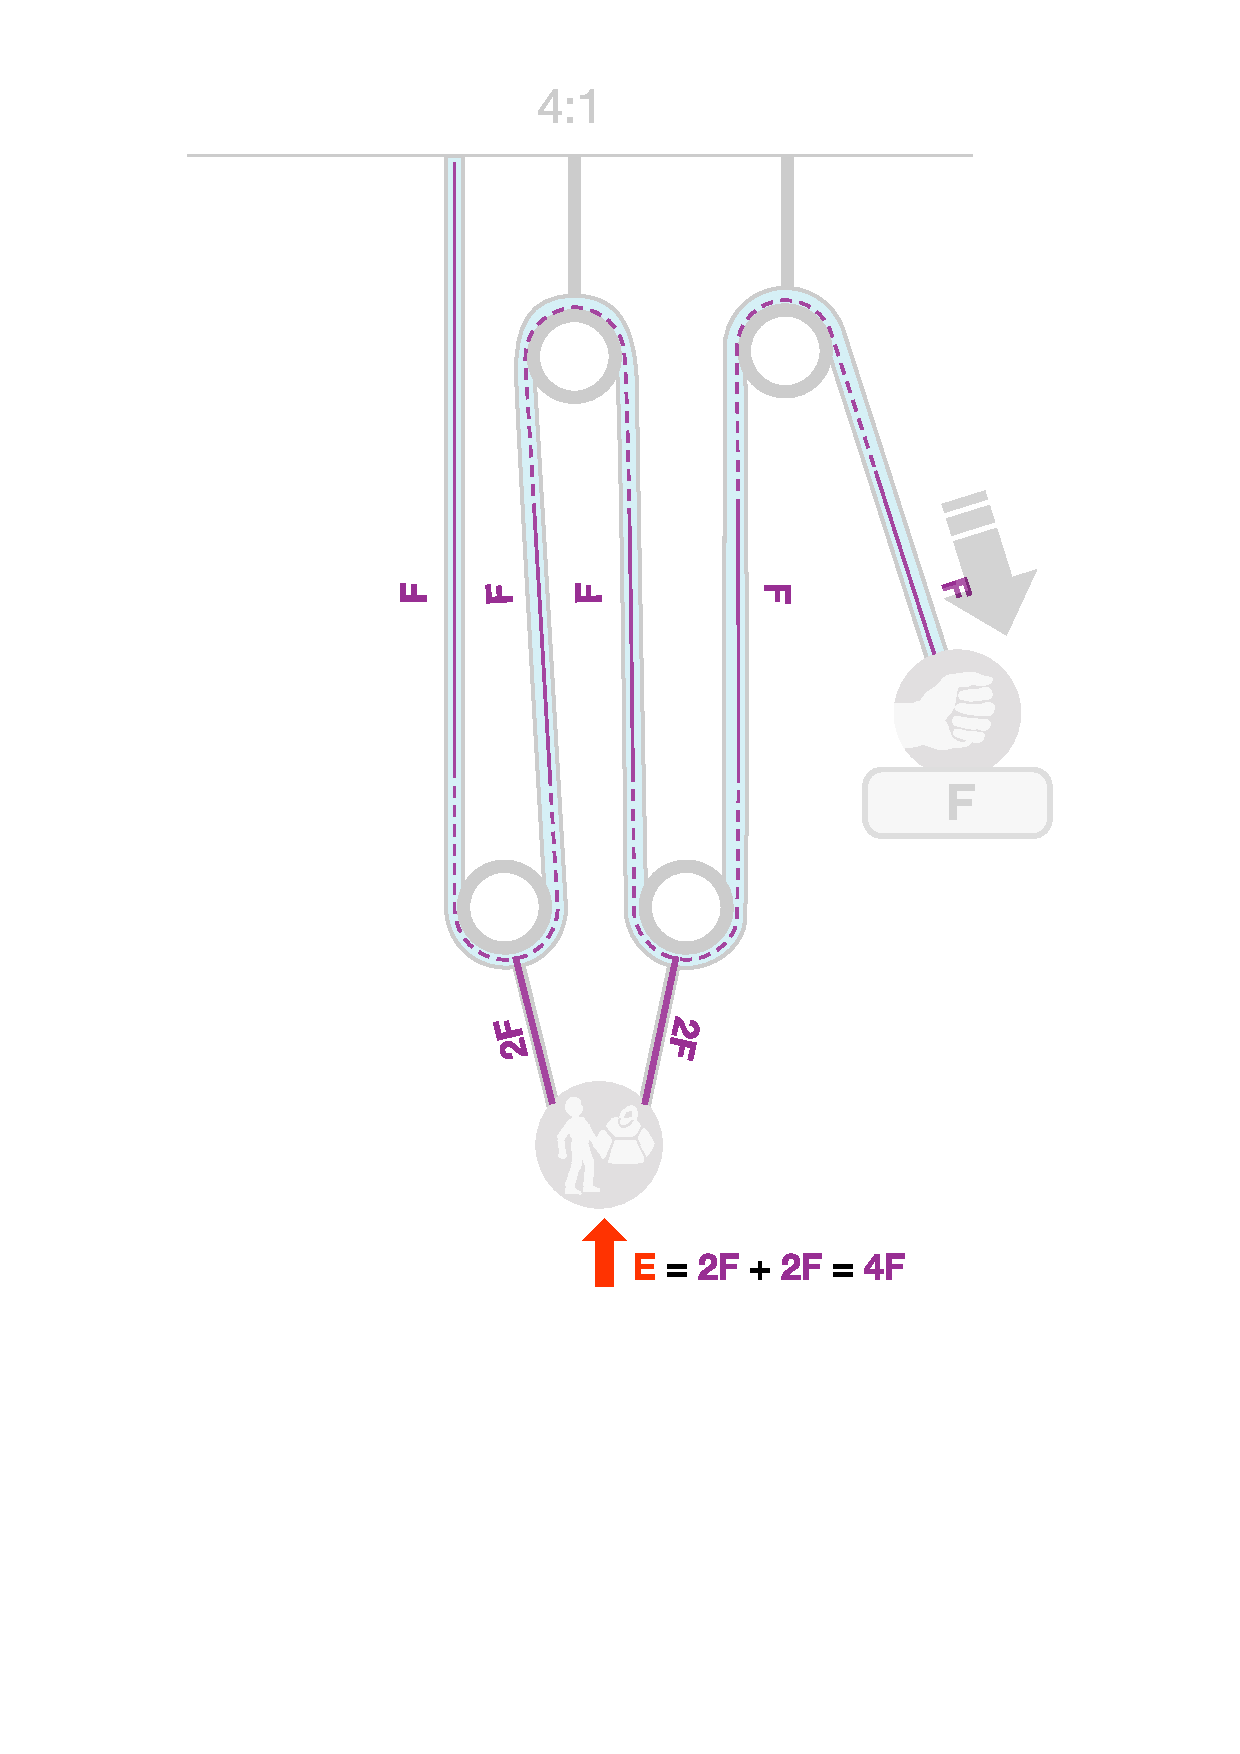
\includegraphics[width=4.0cm]{Figures/4_1/4_haul_system_4_1.pdf}}%
    \caption[Kladkostroj 4:1]{Kladkostroj 4:1 (schéma převzato ze zdroje \cite{Petzl_2022})}
    \label{Obr:4:1}
\end{figure}
%% -------------------------------------------------- %%

\newpage
\subsection{Systém 5:1}
%% -------------------------------------------------- %%
%% -------------------- Pictures --------------------- %%
%% -------------------------------------------------- %%
\begin{figure}[h]
    \centering
    \subcaptionbox{Sestrojení kladkostroje\label{Obr:5:1_Pulley_system}}{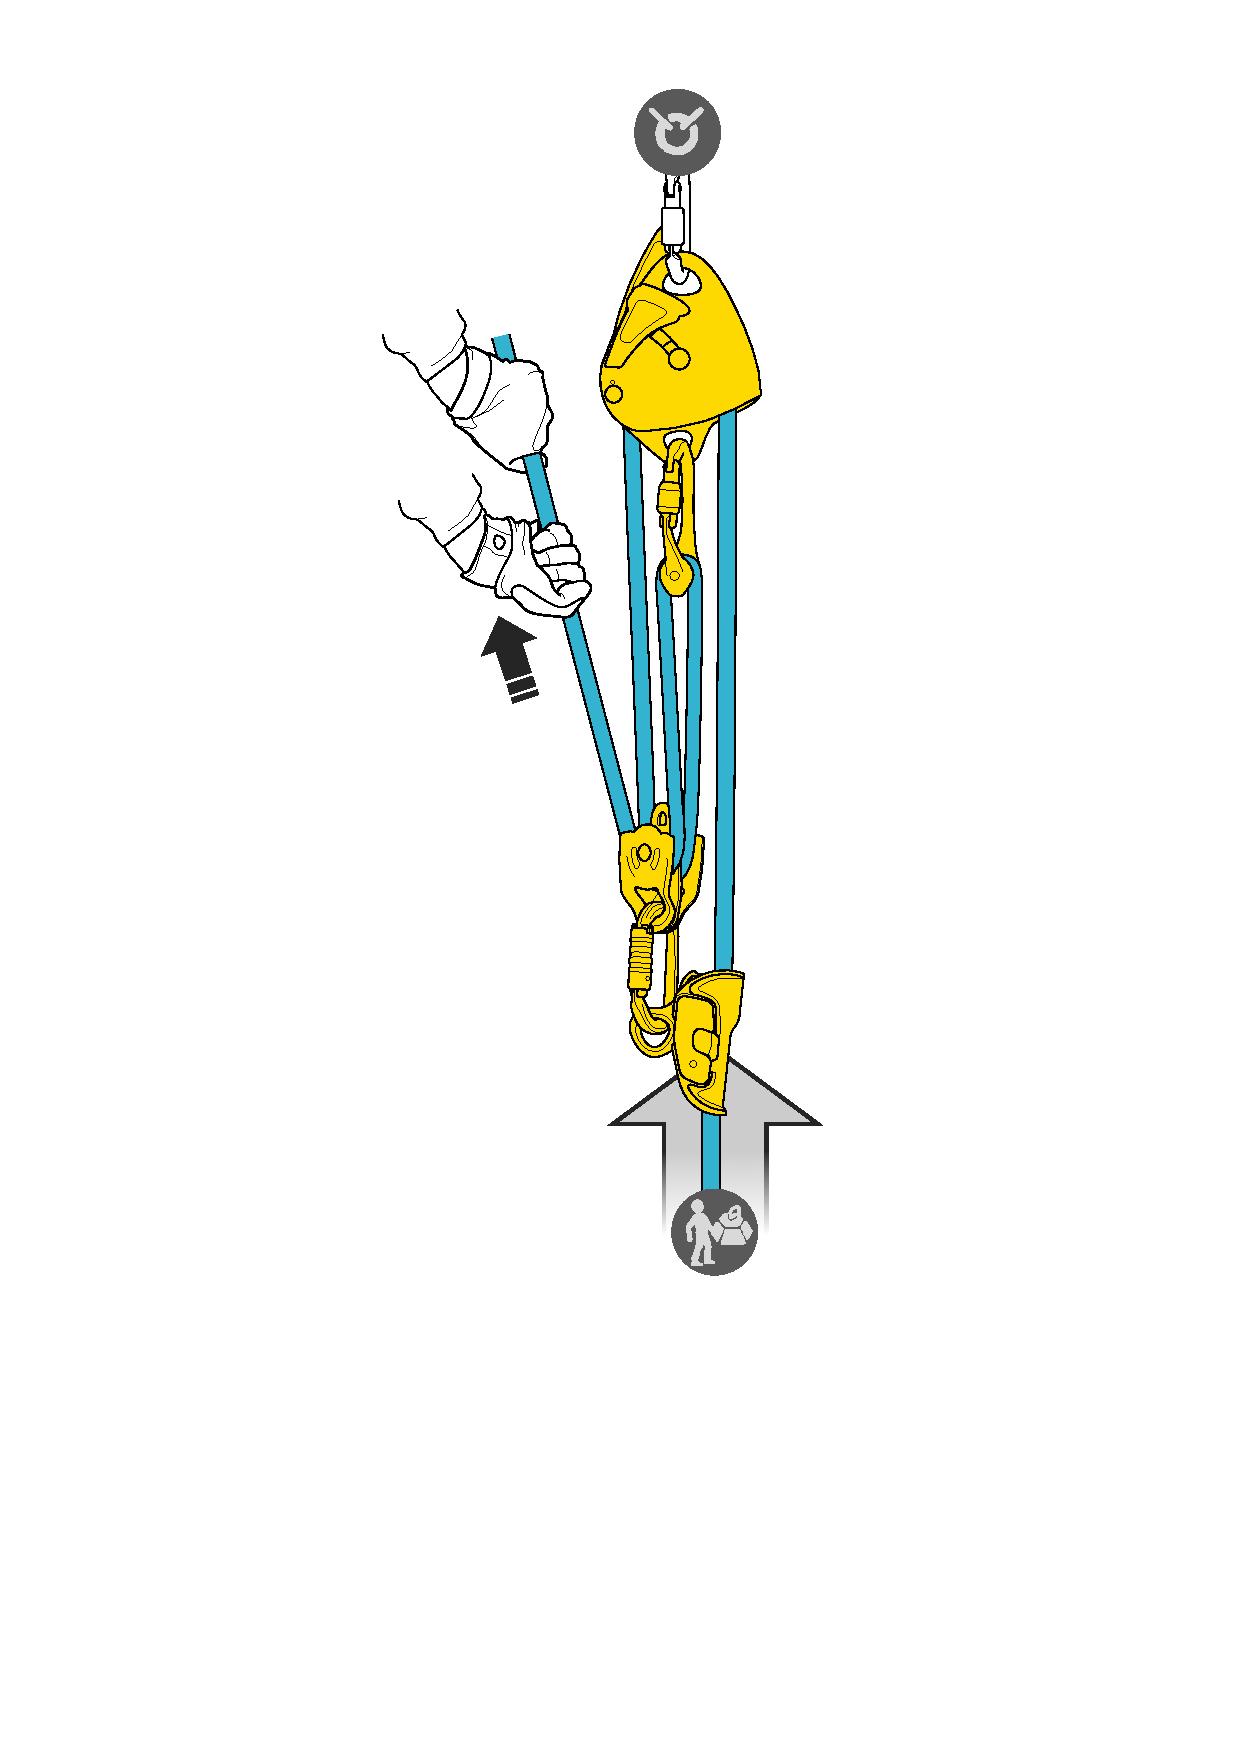
\includegraphics[width=4.0cm]{Figures/5_1/1_haul_system_5_1.pdf}}%
    \hfill % Seperation
    \subcaptionbox{Zobrazení sestrojeného kladkostroje\label{Obr:5:1_Figure_pulley_system}}{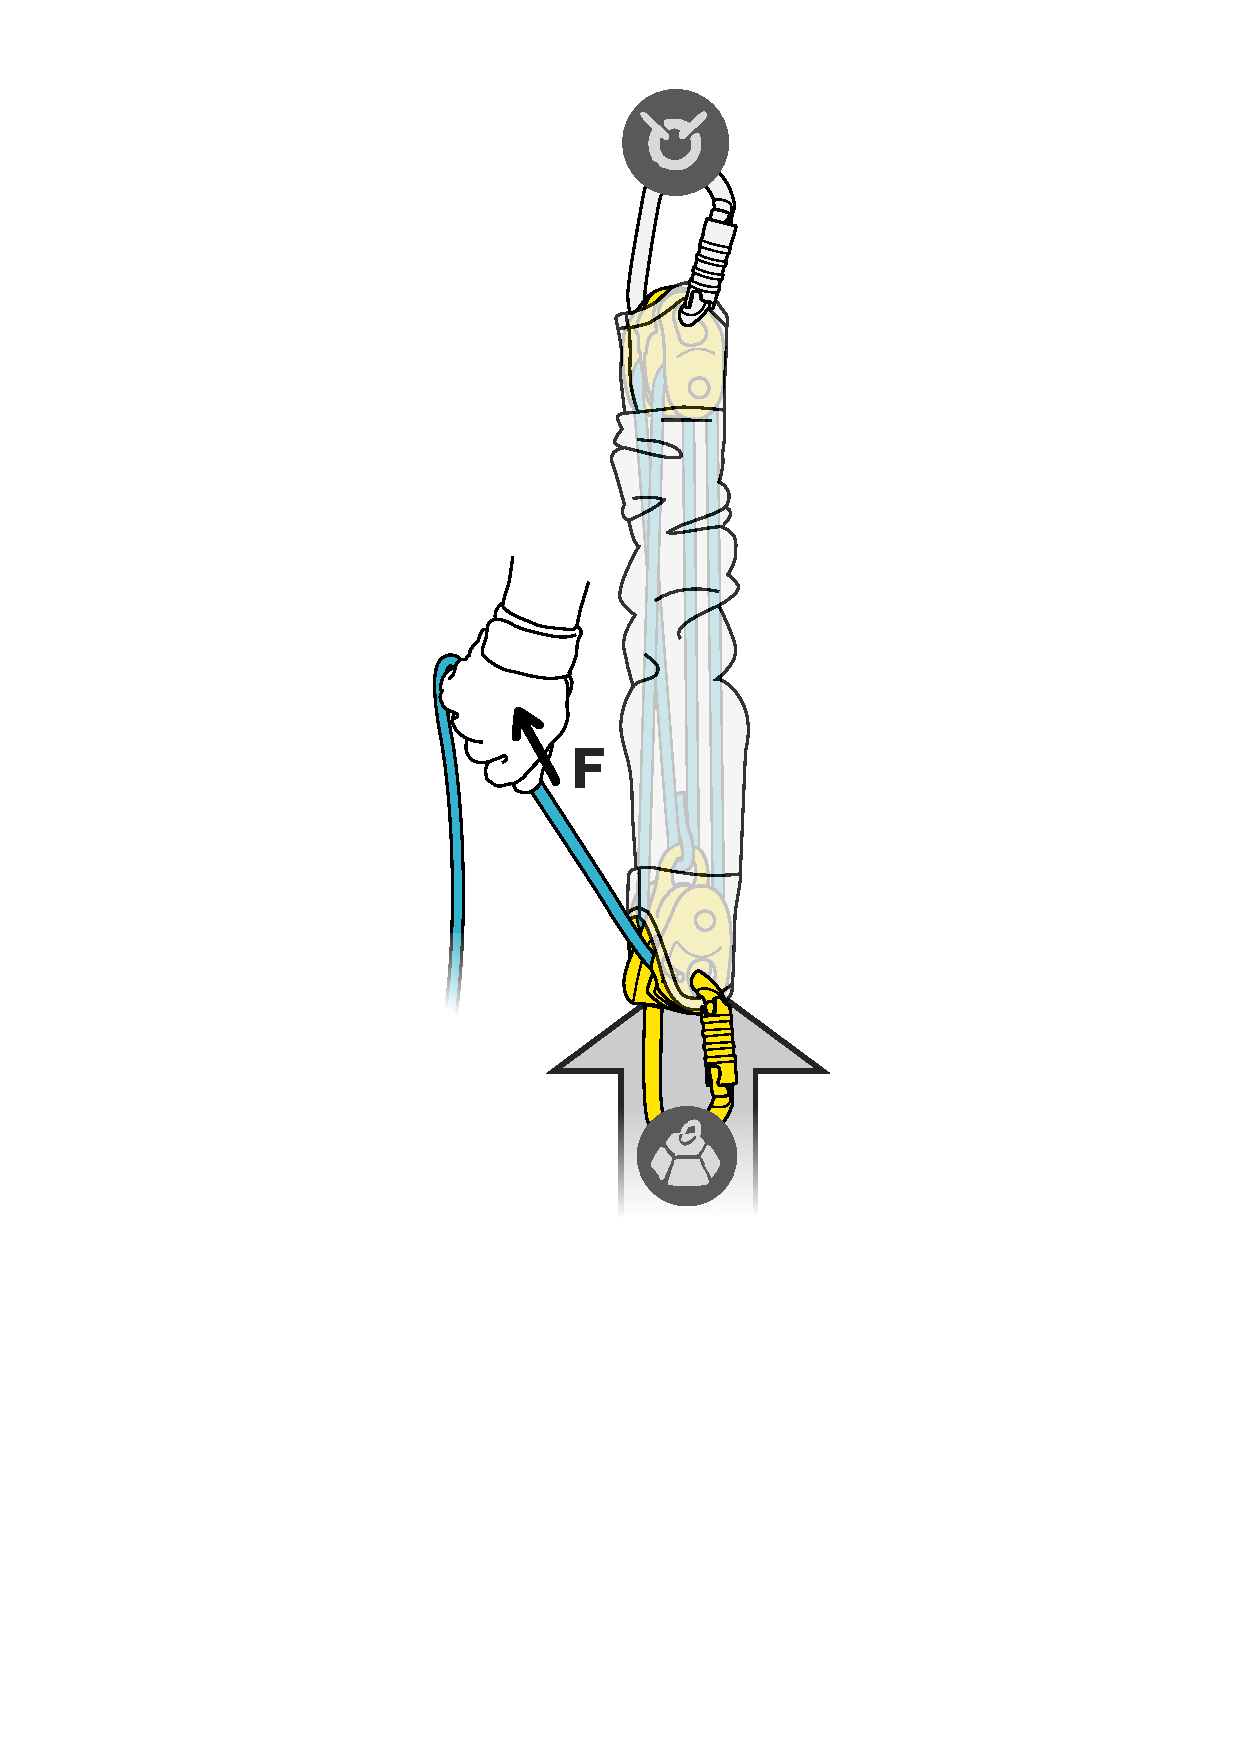
\includegraphics[width=4.0cm]{Figures/5_1/2_haul_system_5_1.pdf}}%
    \\ % Line break
    \subcaptionbox{Schéma kladkostroje\label{Obr:5:1_diagram}}{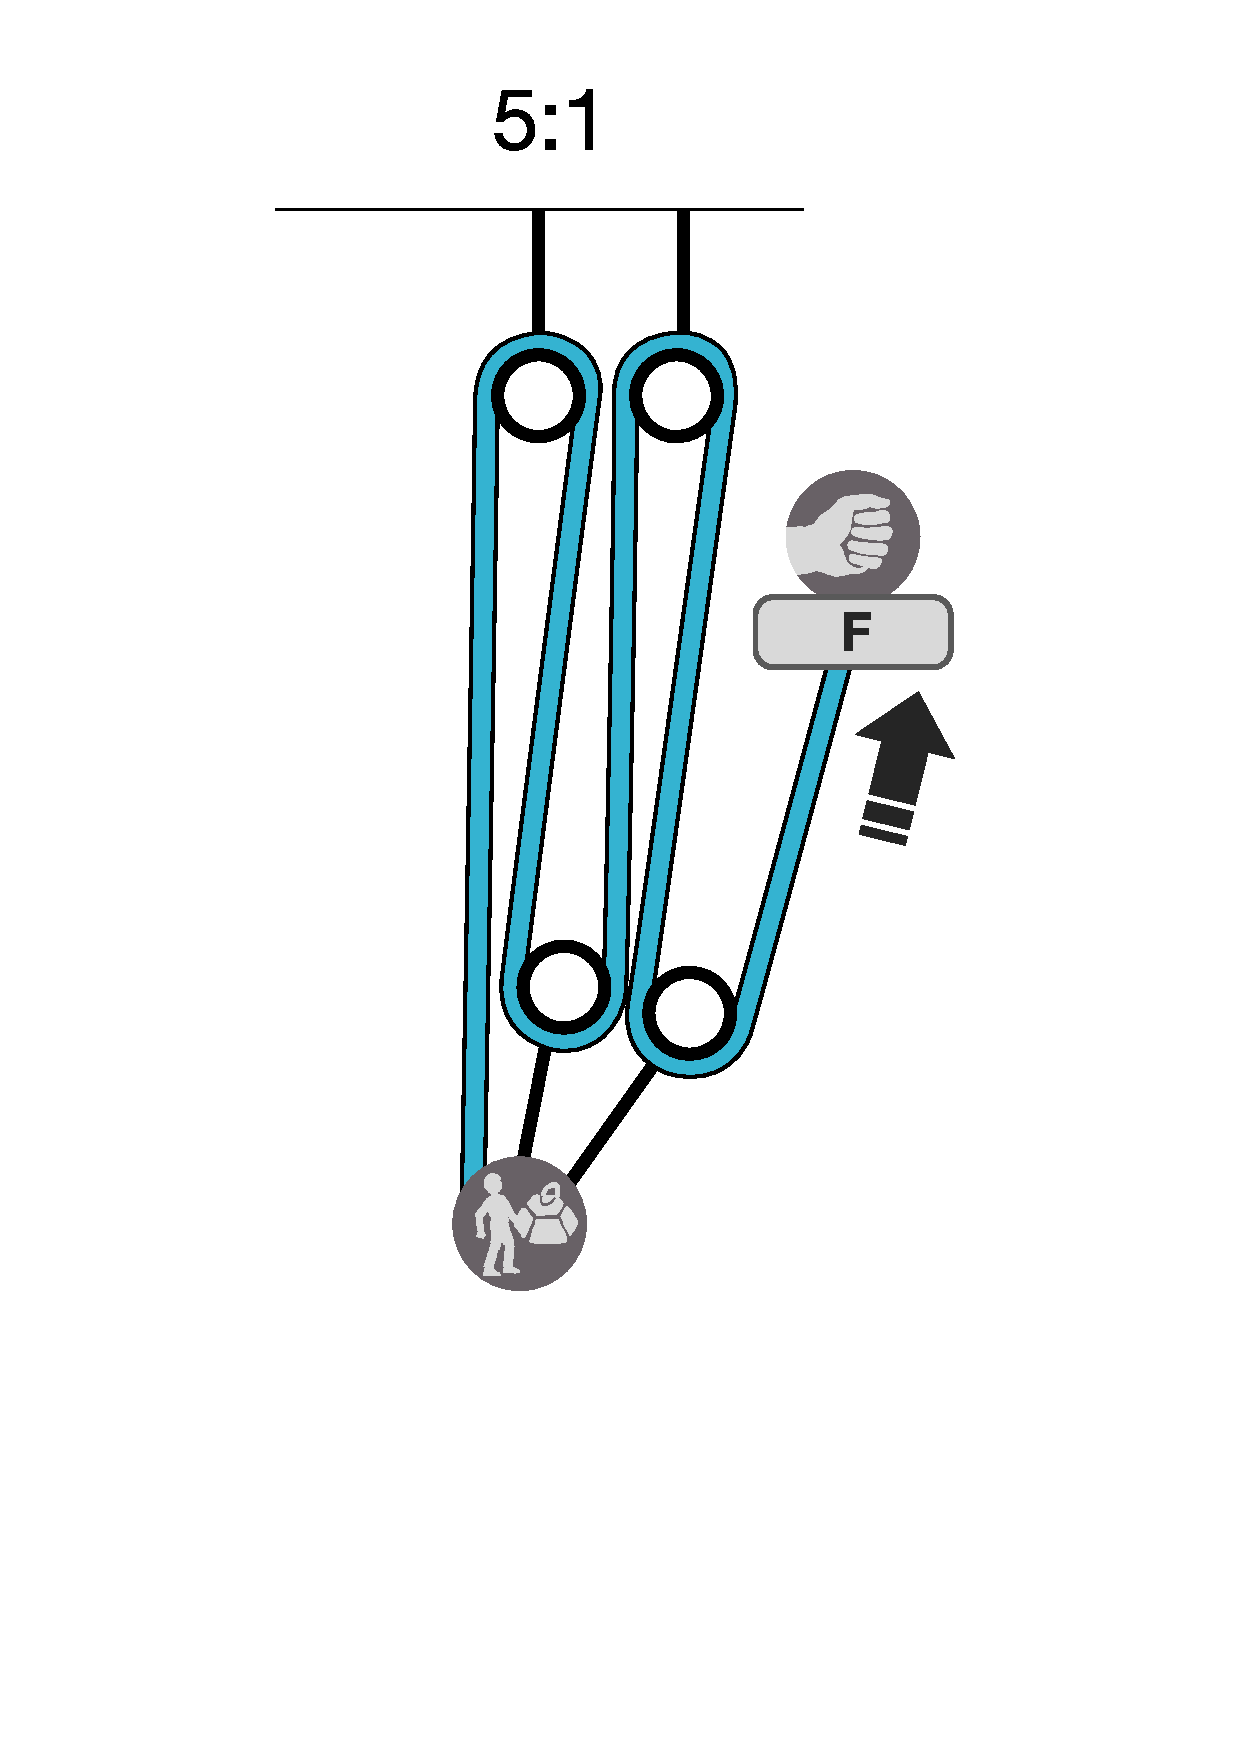
\includegraphics[width=4.0cm]{Figures/5_1/3_haul_system_5_1.pdf}}%
    \hfill % Seperation
    \subcaptionbox{Rozložení sil\label{Obr:5:1_forces_distribution}}{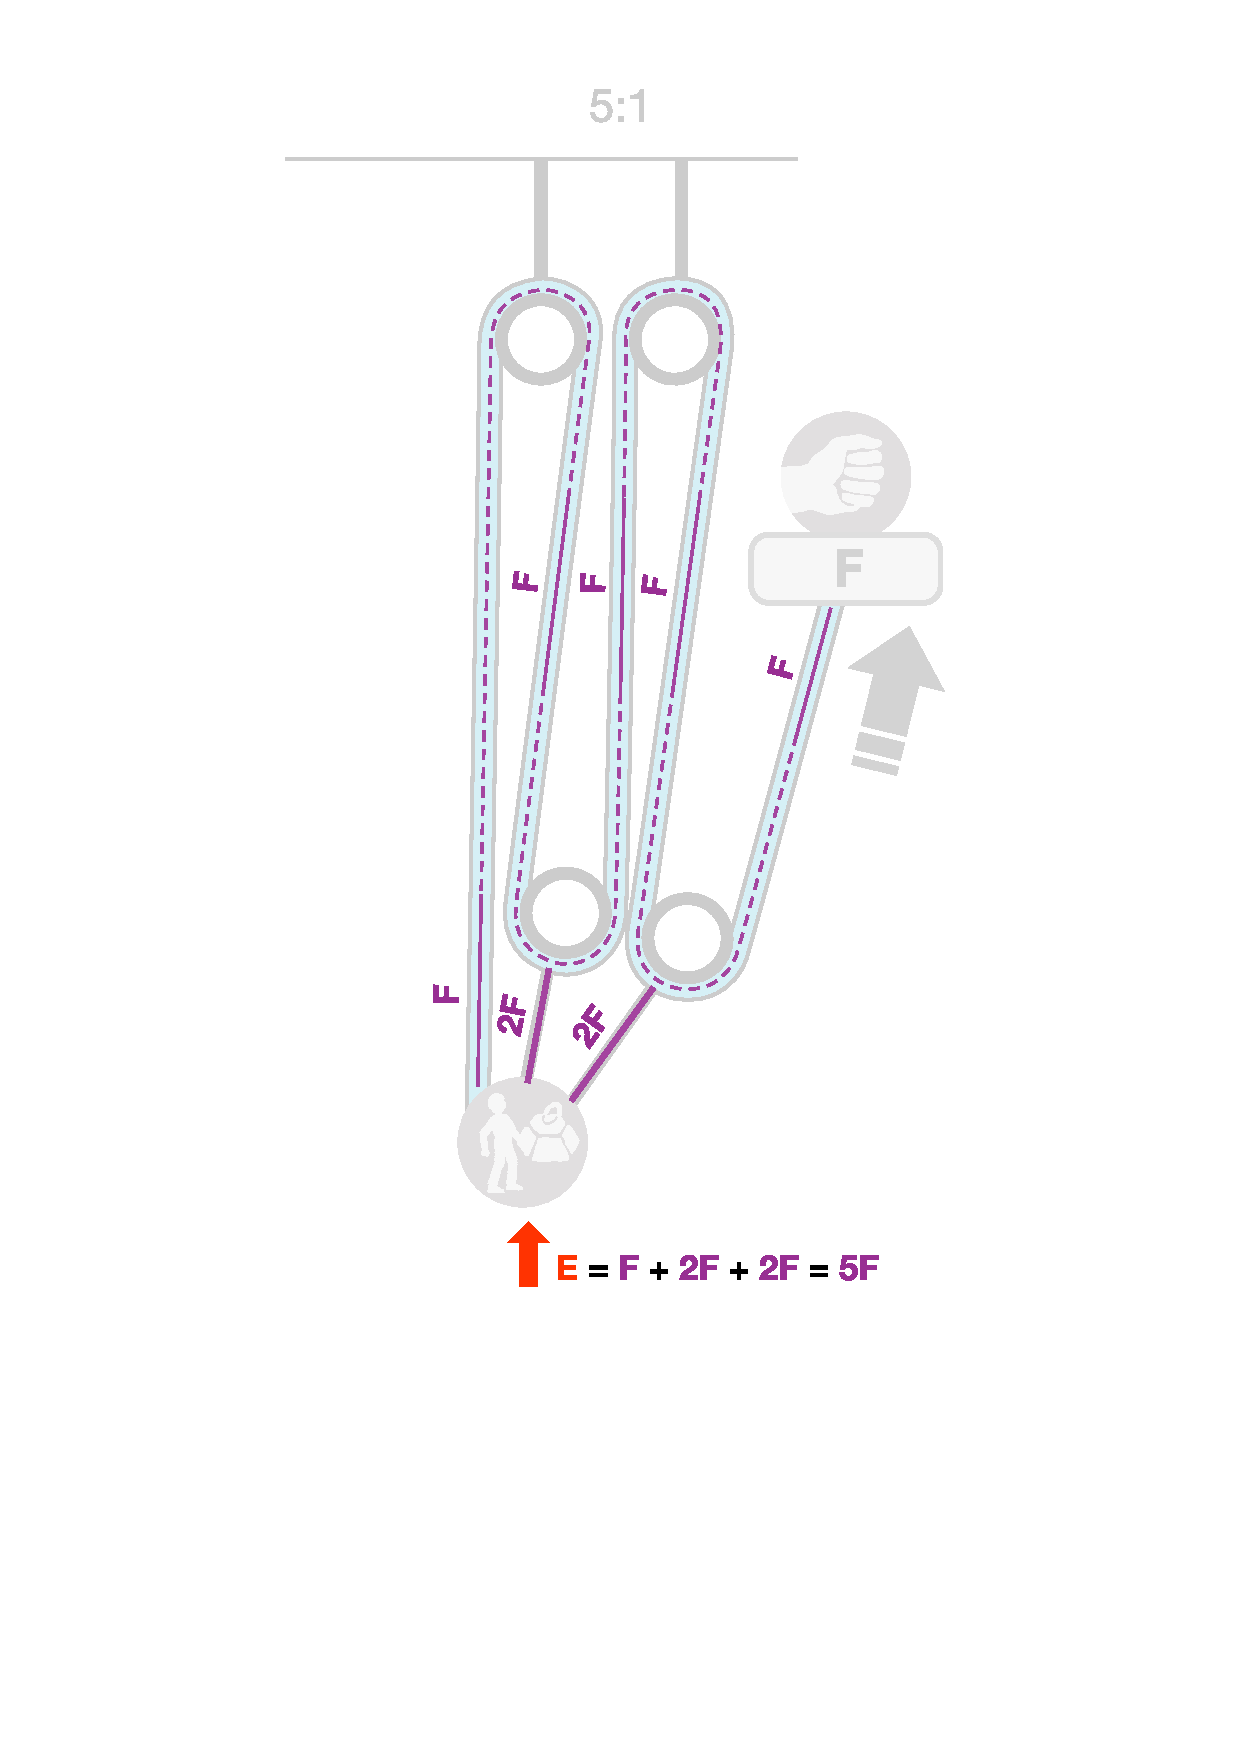
\includegraphics[width=4.0cm]{Figures/5_1/4_haul_system_5_1.pdf}}%
    \caption[Kladkostroj 5:1]{Kladkostroj 5:1 (schéma převzato ze zdroje \cite{Petzl_2022})}
    \label{Obr:5:1}
\end{figure}
%% -------------------------------------------------- %%

\newpage
\subsection{Systém 7:1}
%% -------------------------------------------------- %%
%% -------------------- Pictures --------------------- %%
%% -------------------------------------------------- %%
\begin{figure}[h]
    \centering
    \subcaptionbox{Sestrojení kladkostroje\label{Obr:7:1_Pulley_system}}{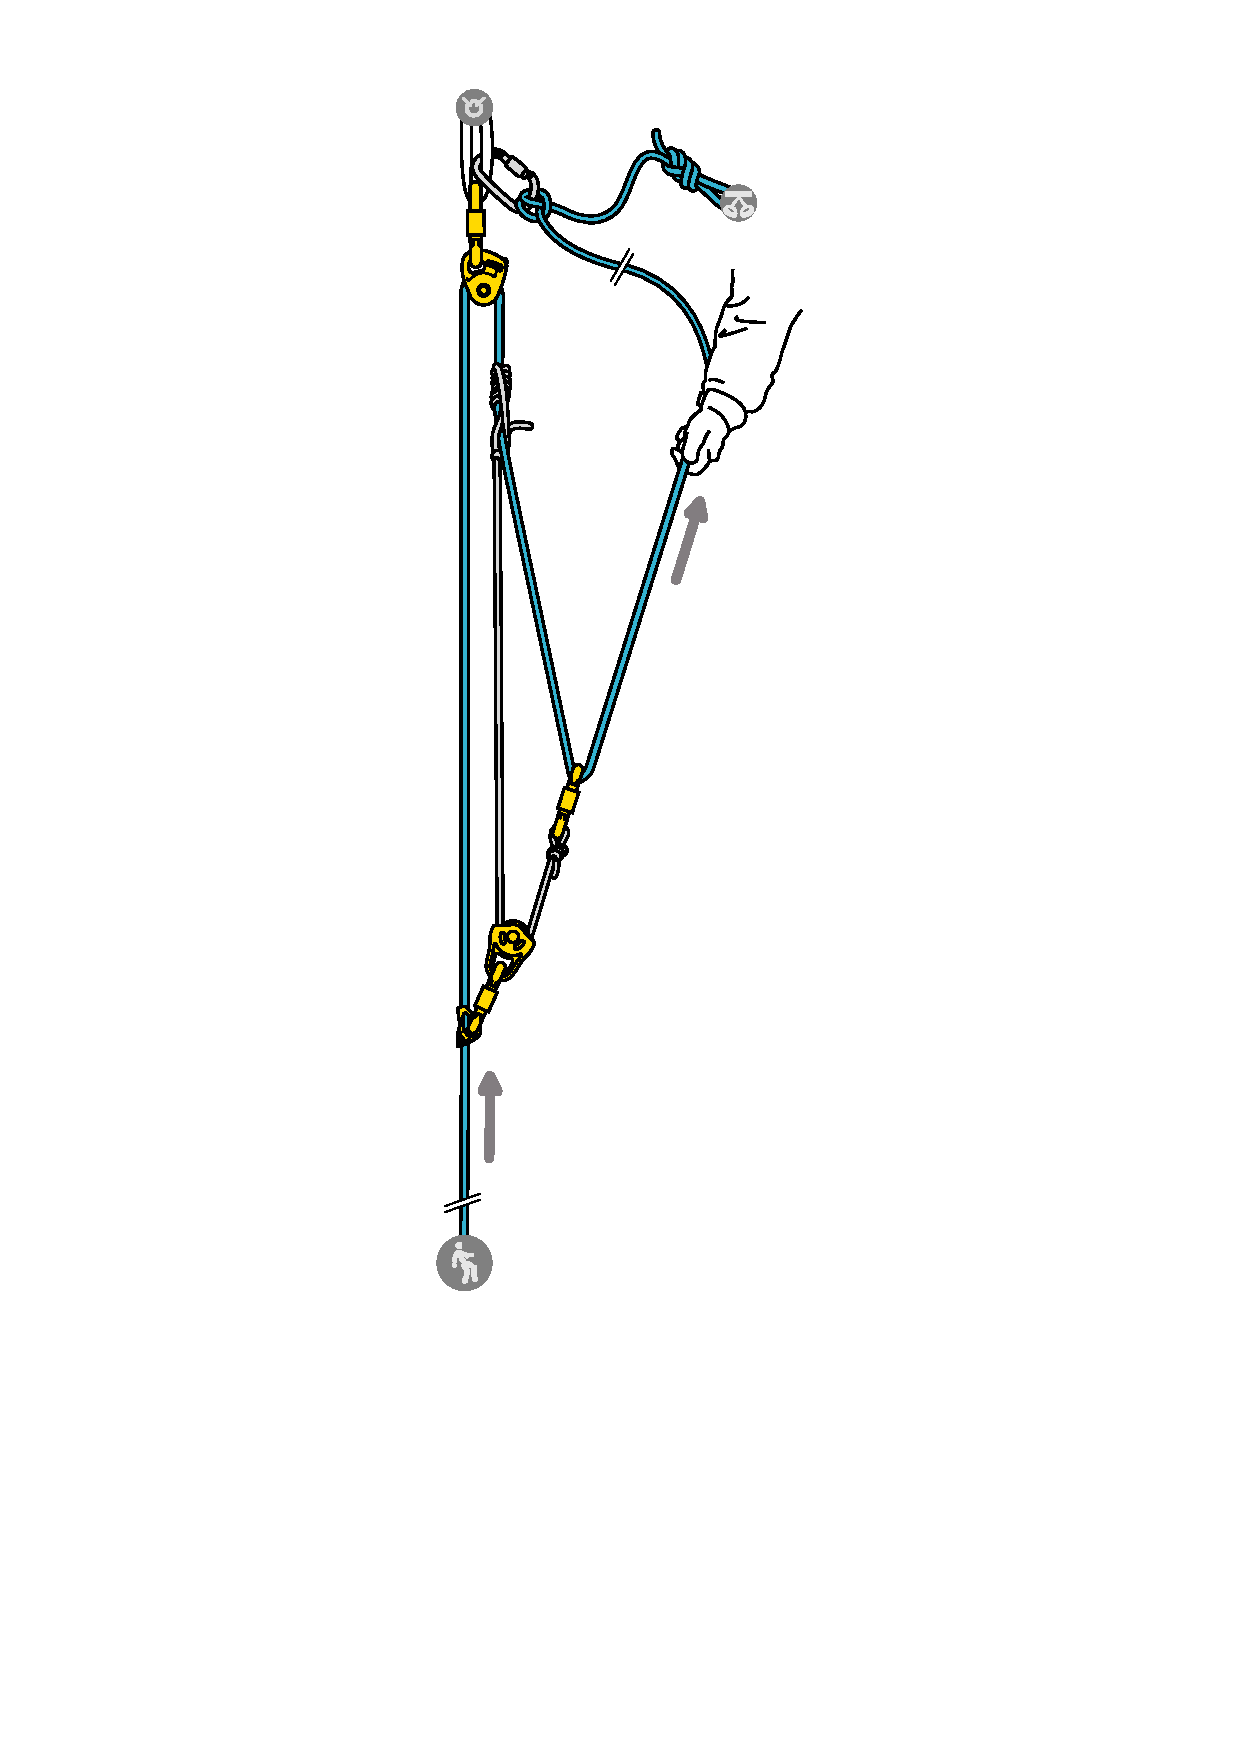
\includegraphics[width=4.0cm]{Figures/7_1/1_haul_system_7_1.pdf}}%
    \hfill % Seperation
    \subcaptionbox{Schéma kladkostroje\label{Obr:7:1_diagram}}{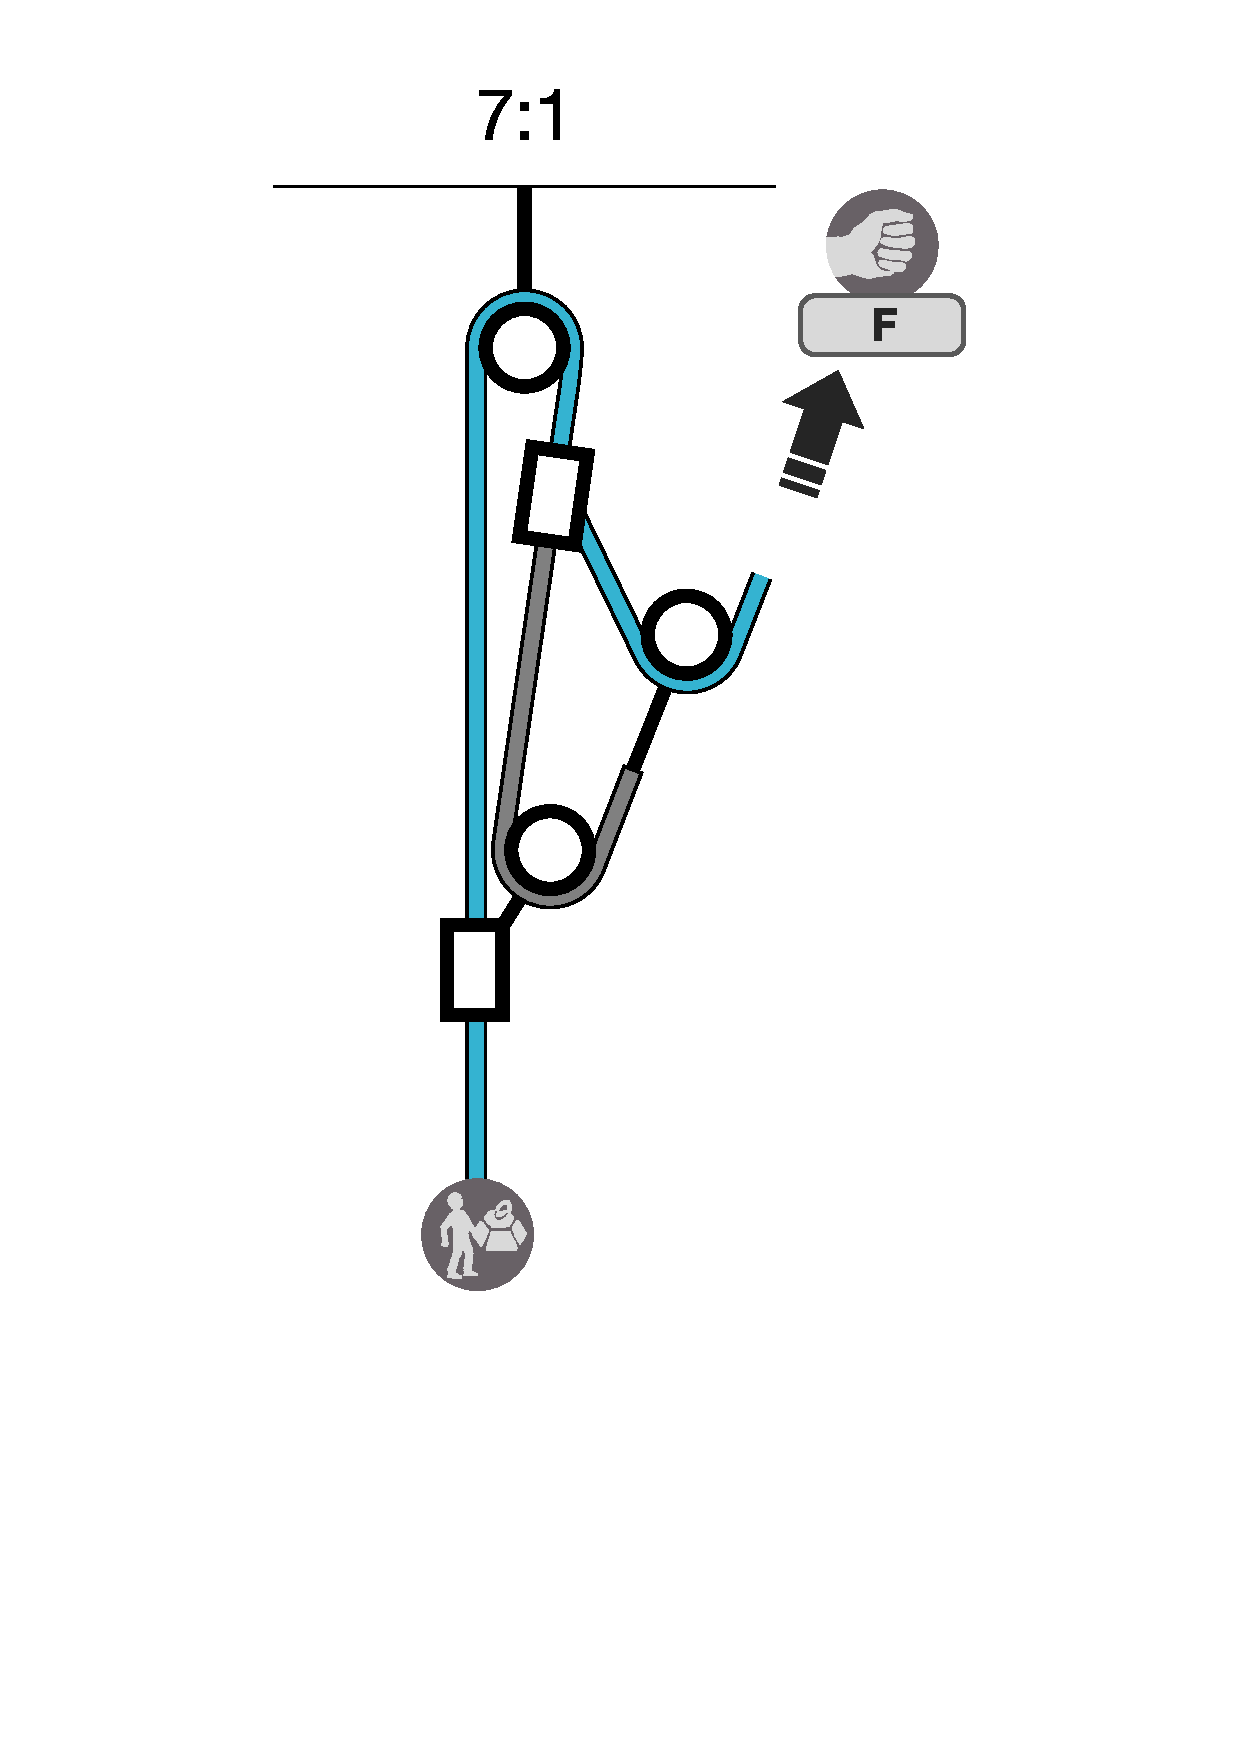
\includegraphics[width=4.0cm]{Figures/7_1/2_haul_system_7_1.pdf}}%
    \\ % Line break
    \subcaptionbox{Rozložení sil\label{Obr:7:1_forces_distribution}}{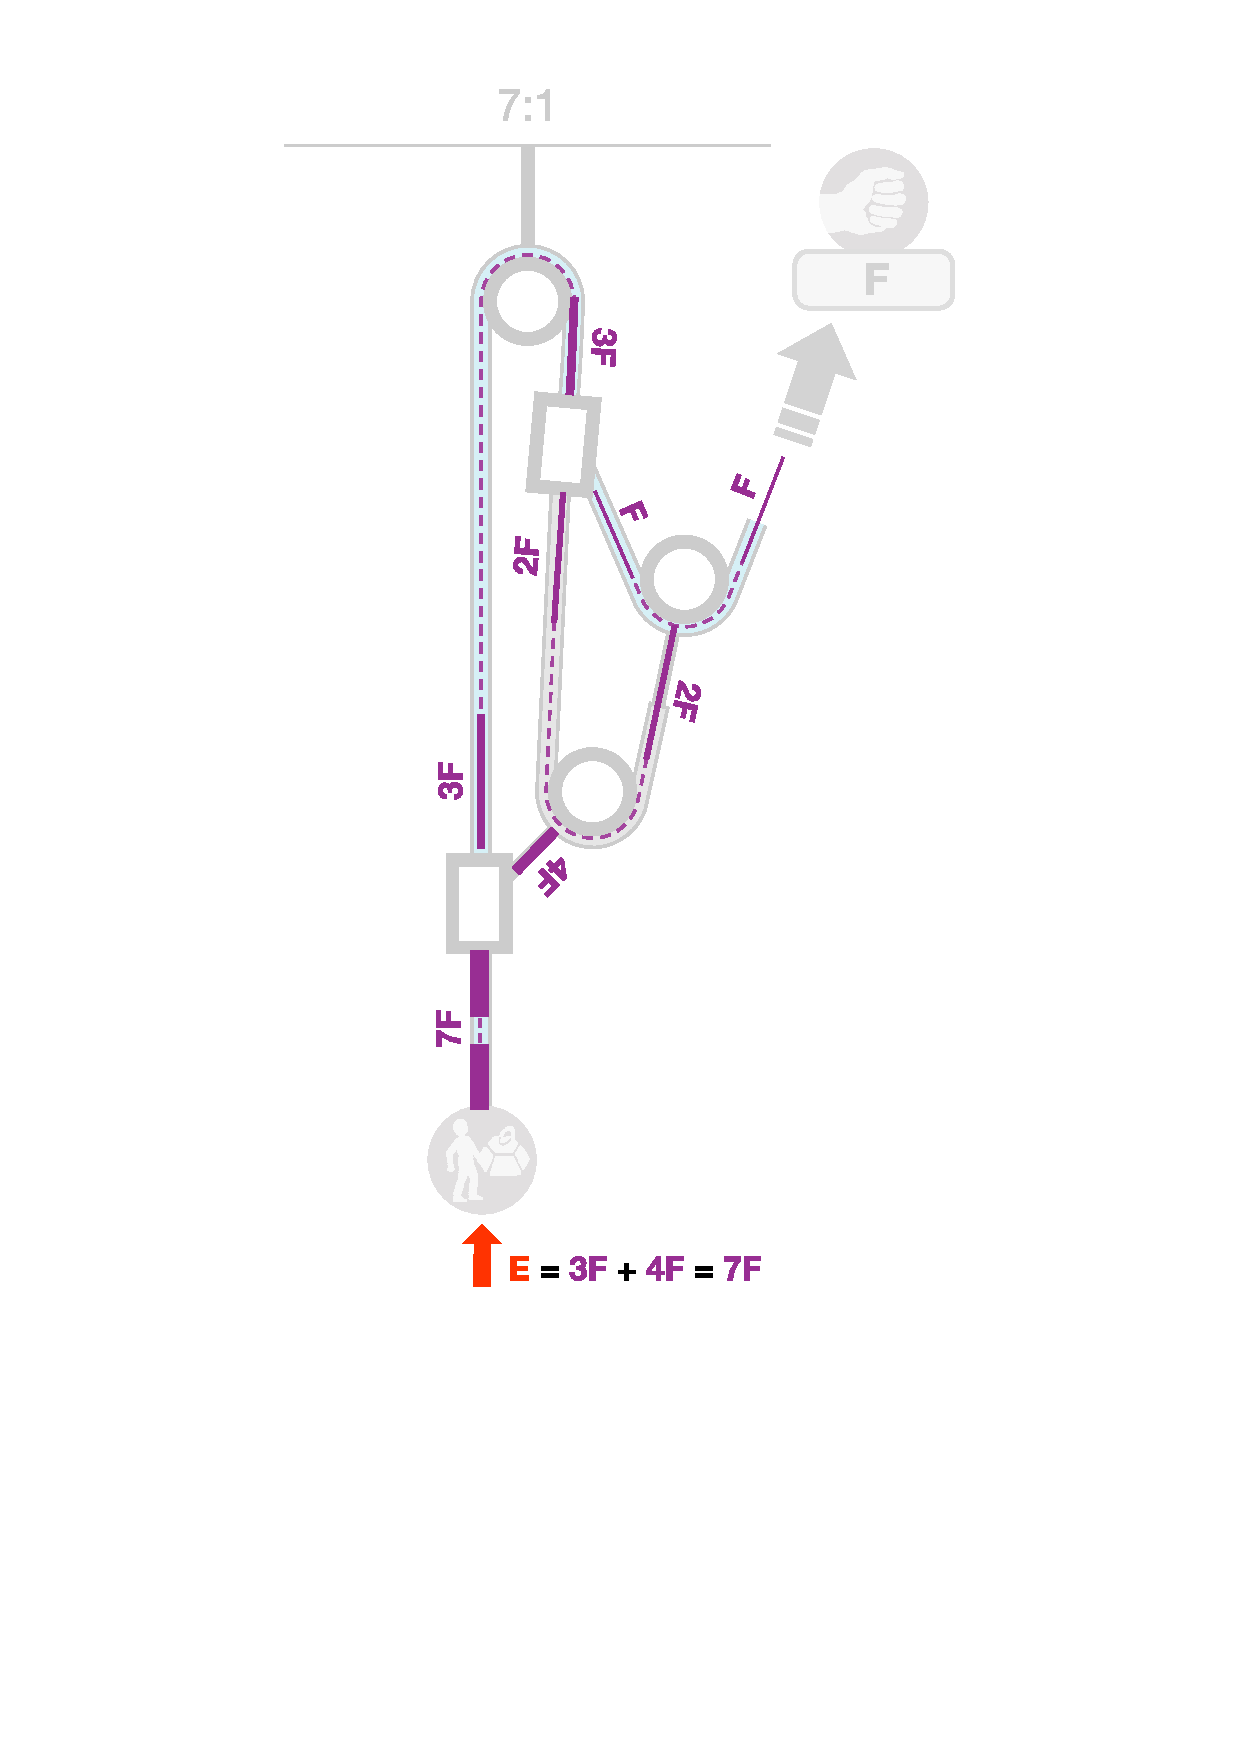
\includegraphics[width=4.0cm]{Figures/7_1/3_haul_system_7_1.pdf}}%
    \caption[Kladkostroj 7:1]{Kladkostroj 7:1 (schéma převzato ze zdroje \cite{Petzl_2022})}
    \label{Obr:7:1}
\end{figure}
%% -------------------------------------------------- %%
\section{Popis kladkostrojů}
\subsection{Systém volné kladky "Loserolle"}

Tato technika je využívána zejména při záchraně na ledovci. Nejjednoduší použití této metody je pokud je lezec při vědomí. Pokud je lezec zraněný nebo není při vědomí musíme se nejdříve k lezci slanit a až poté jej vytahovat za pomocí kladky nahoru. 
\\
\\
Postup:

1. Zřídíme stanoviště - vykopeme díru například pro vložení cepínu. Na topůrko cepínu uvážeme liščí smyčkou sešitou smyčku (viz~\autoref{Obr:Snow_anchor}). Následně cepín zakopeme a pomocí prusíku, který máme navázaný na laně uvolníme ze sebe zátěž a přeneseme ji na nově vybudované stanoviště.

2. Na volném prameni lana umístíme 3\,m prusík pro sebezajištění.

3. Na volném prameni dojdeme na kraj trhliny, celou dobu jsme jištěni prusíkem. Na volném prameni lana spustíme karabinu (kladku) k zachraňovanému lezci, který si karabinu cvakne do sedáku.

4. Prusík, který posloužil pro odtížení váhy lezce bude sloužit jako zajištění vytahovaného lana, takový to jednoduchý kladkostroj by fungoval s účinností systému 2:1 (viz~\autoref{Obr:Crevasse_2:1}). 

5. Pokud bychom volné lano ve zřízeném stanovišti zajistili prusíkem, tiblocem nebo microtraxtionem a dále použili prusík s karabinou popřípadě tibloc s karabinou a kladkou vytvořili bychom systém 6:1 (viz~\autoref{Obr:Crevasse_6:1}). Další možností je vytvořit systém 3:1 (viz~\autoref{Obr:Crevasse_3:1}) nebo 7:1 (viz~\autoref{Obr:Crevasse_7:1}) \cite{climbing_school_2022}.
\\
\\
Nejčastější chyby:

1. Celý systém je zajištěn pouze přes jeden prusík.

2. Chybné nastavení délek prusíků.

3. Překřížení pramenů lana v systému.
%% -------------------------------------------------- %%
%% -------------------- Pictures --------------------- %%
%% -------------------------------------------------- %%
\begin{figure}[h]
    \centering
    {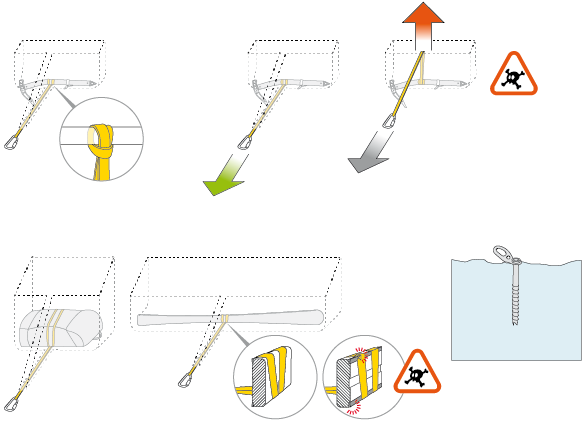
\includegraphics[width=8.0cm]{Figures/Crevasse/Snow_anchor.png}}%
    \caption[Snehova_kotva]{Sněhová kotva (schéma převzato ze zdroje \cite{Petzl_2022})}
    \label{Obr:Snow_anchor}
\end{figure}
%% -------------------------------------------------- %%
%% -------------------- Pictures --------------------- %%
%% -------------------------------------------------- %%
\begin{figure}[h]
    \centering
    {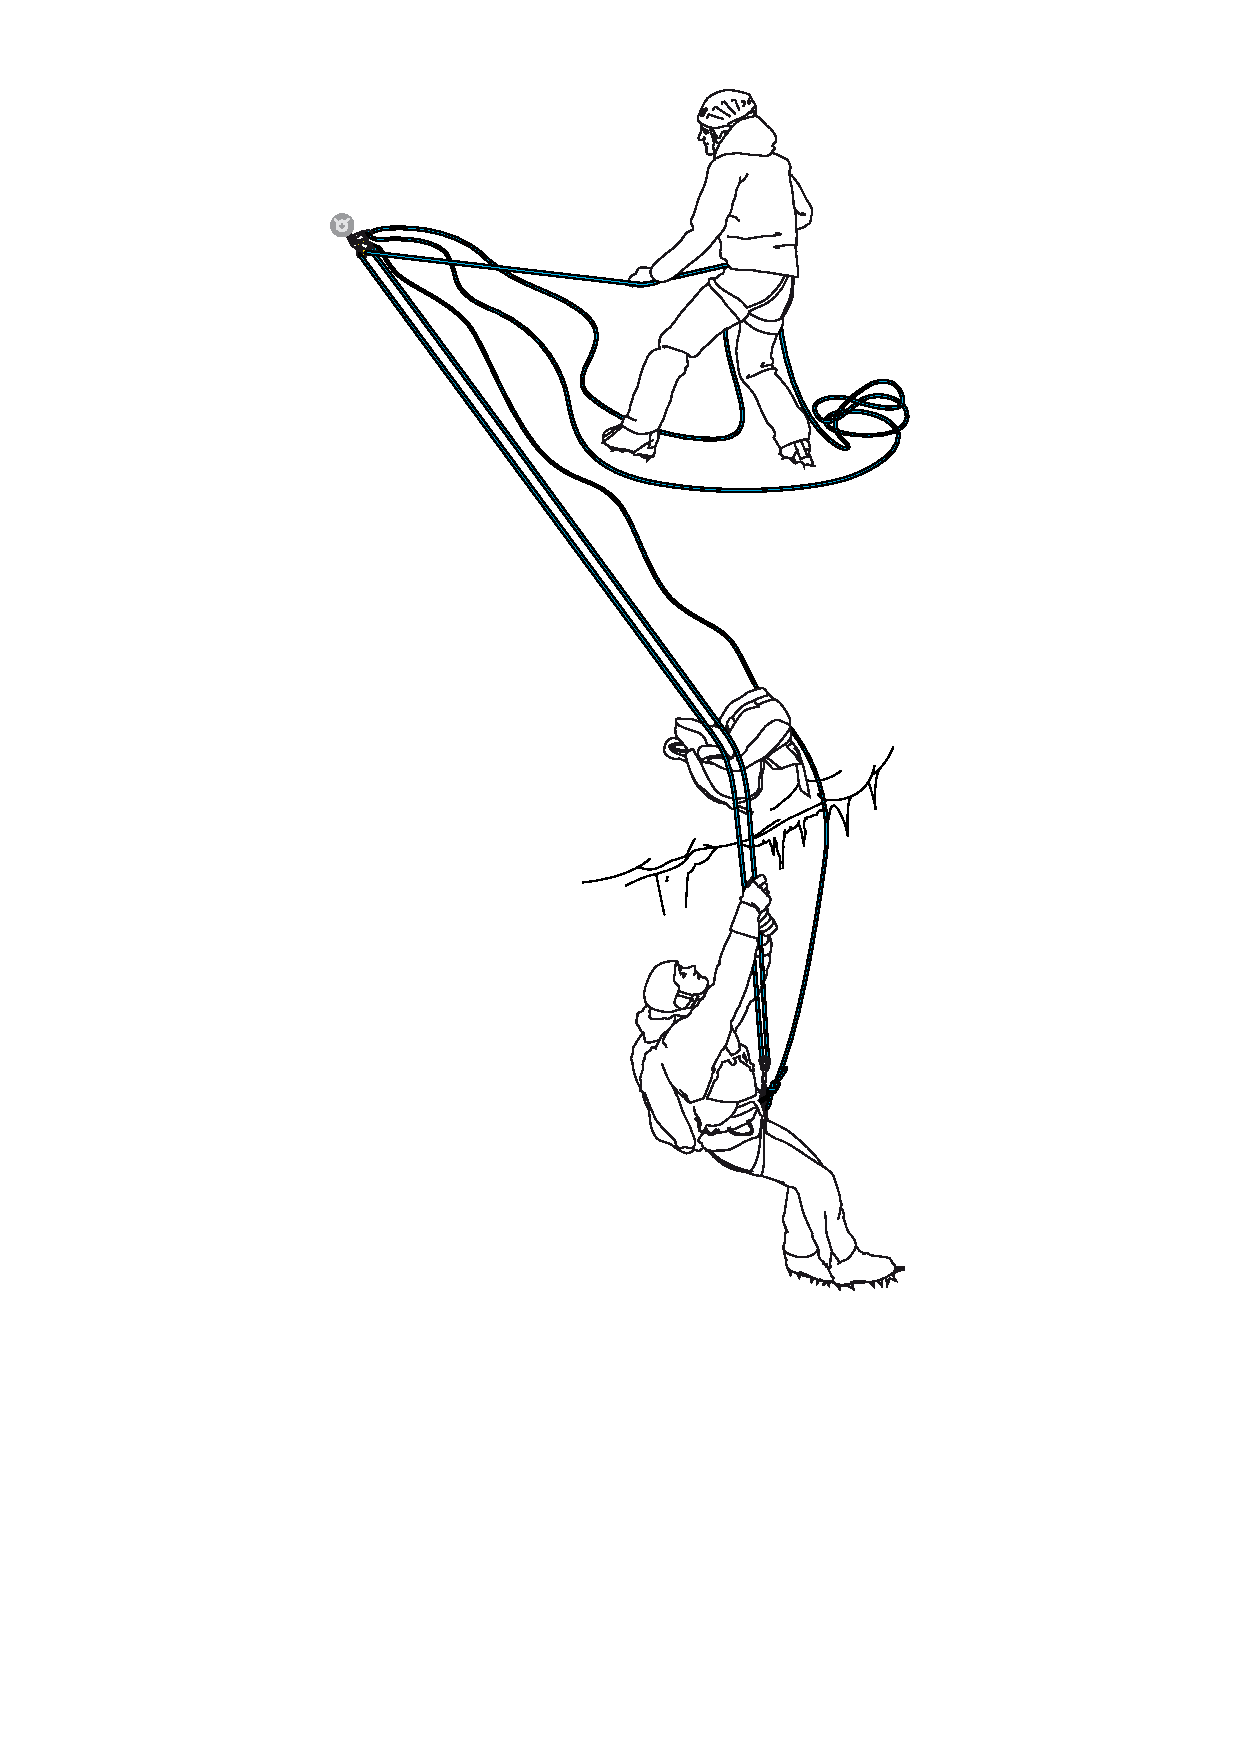
\includegraphics[width=8.0cm]{Figures/Crevasse/1_Petzl_Crevasse_haul_system_2_1.pdf}}%
    \caption[Crevasse 2:1]{Záchrana z ledovcové trhliny 2:1 (schéma převzato ze zdroje \cite{Petzl_2022})}
    \label{Obr:Crevasse_2:1}
\end{figure}
%% -------------------------------------------------- %%
%% -------------------- Pictures --------------------- %%
%% -------------------------------------------------- %%
\begin{figure}[h]
    \centering
    {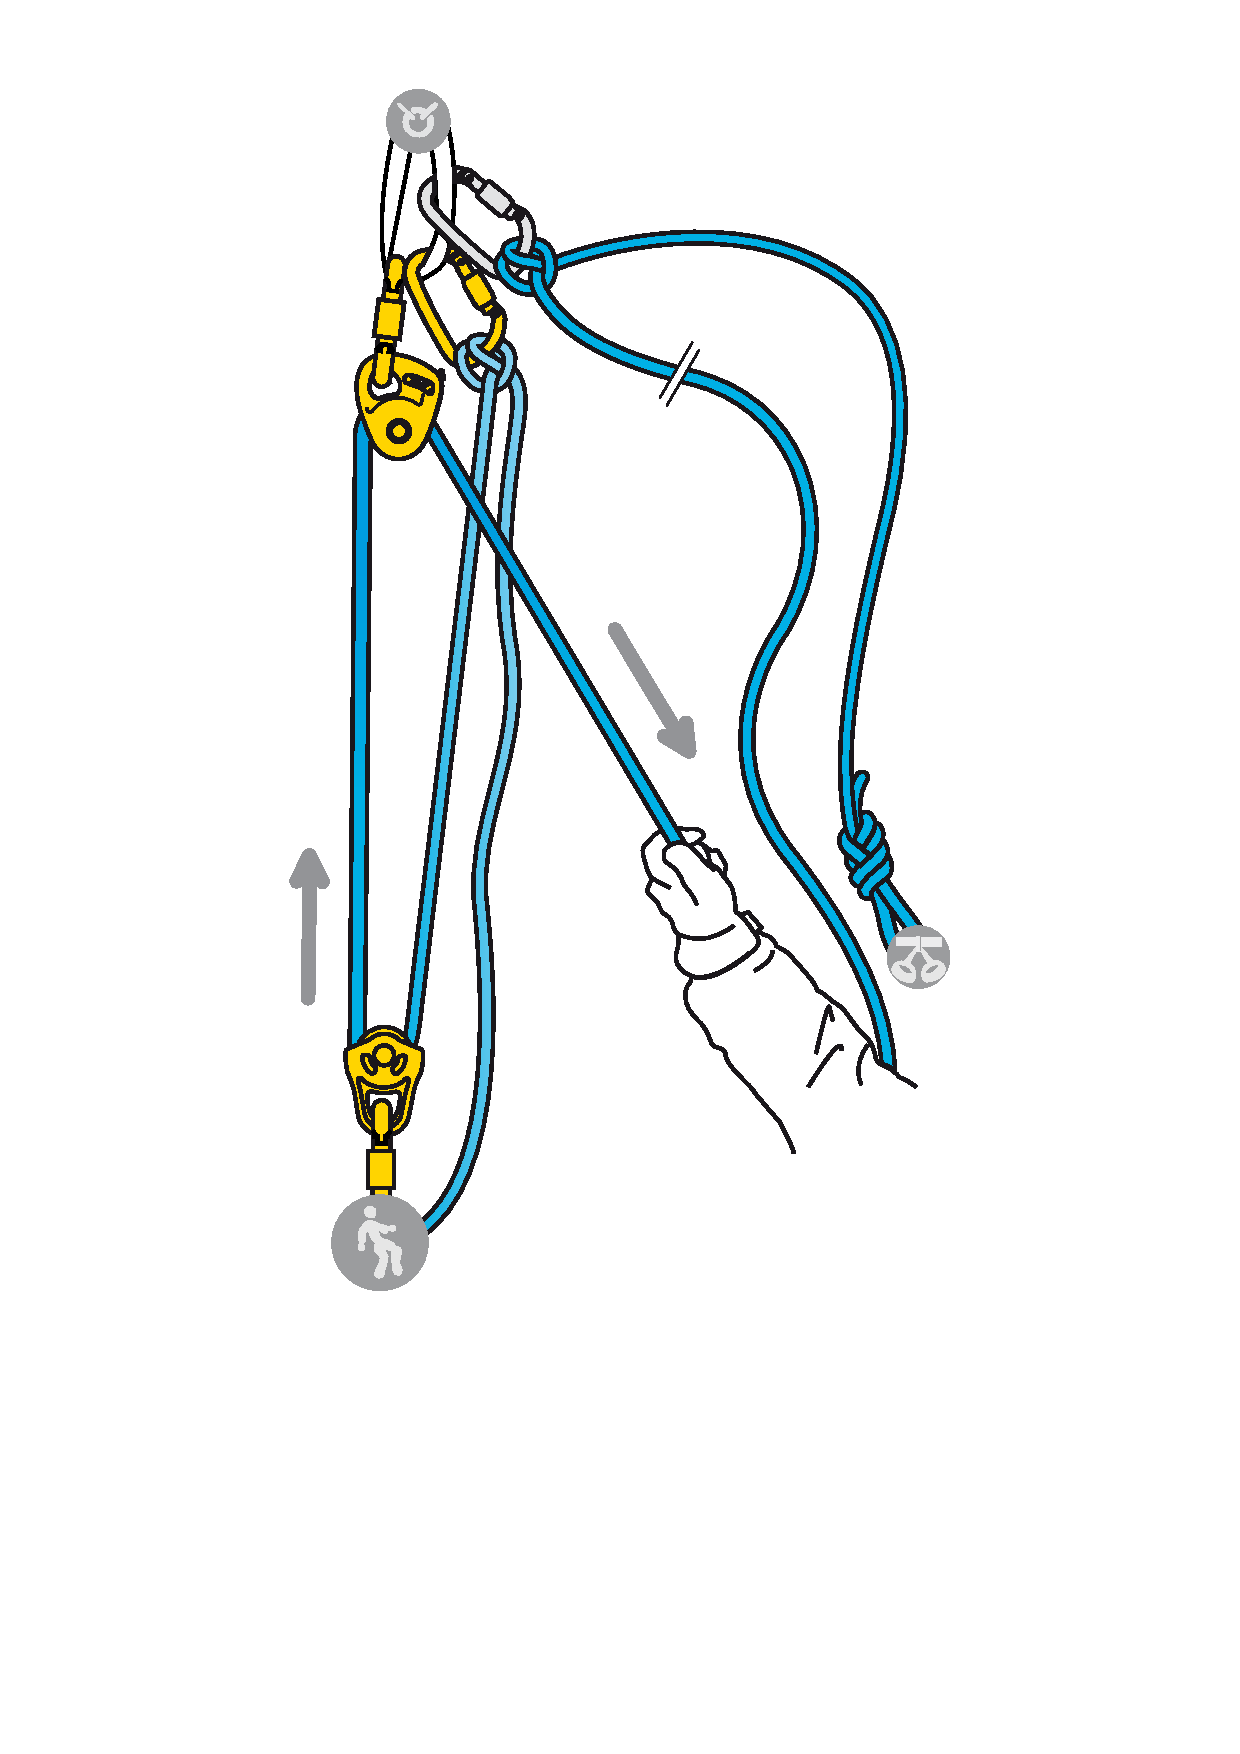
\includegraphics[width=4.0cm]{Figures/Crevasse/1_Petzl_Crevasse_haul_system_2_1_detail.pdf}}%
    \caption[Crevasse 2:1 detail]{Detail kladkostroje pro záchranu z ledovcové trhliny 2:1 (schéma převzato ze zdroje \cite{Petzl_2022})}
    \label{Obr:Crevasse_2:1_detail}
\end{figure}
%% -------------------------------------------------- %%
%% -------------------- Pictures --------------------- %%
%% -------------------------------------------------- %%
\begin{figure}[h]
    \centering
    {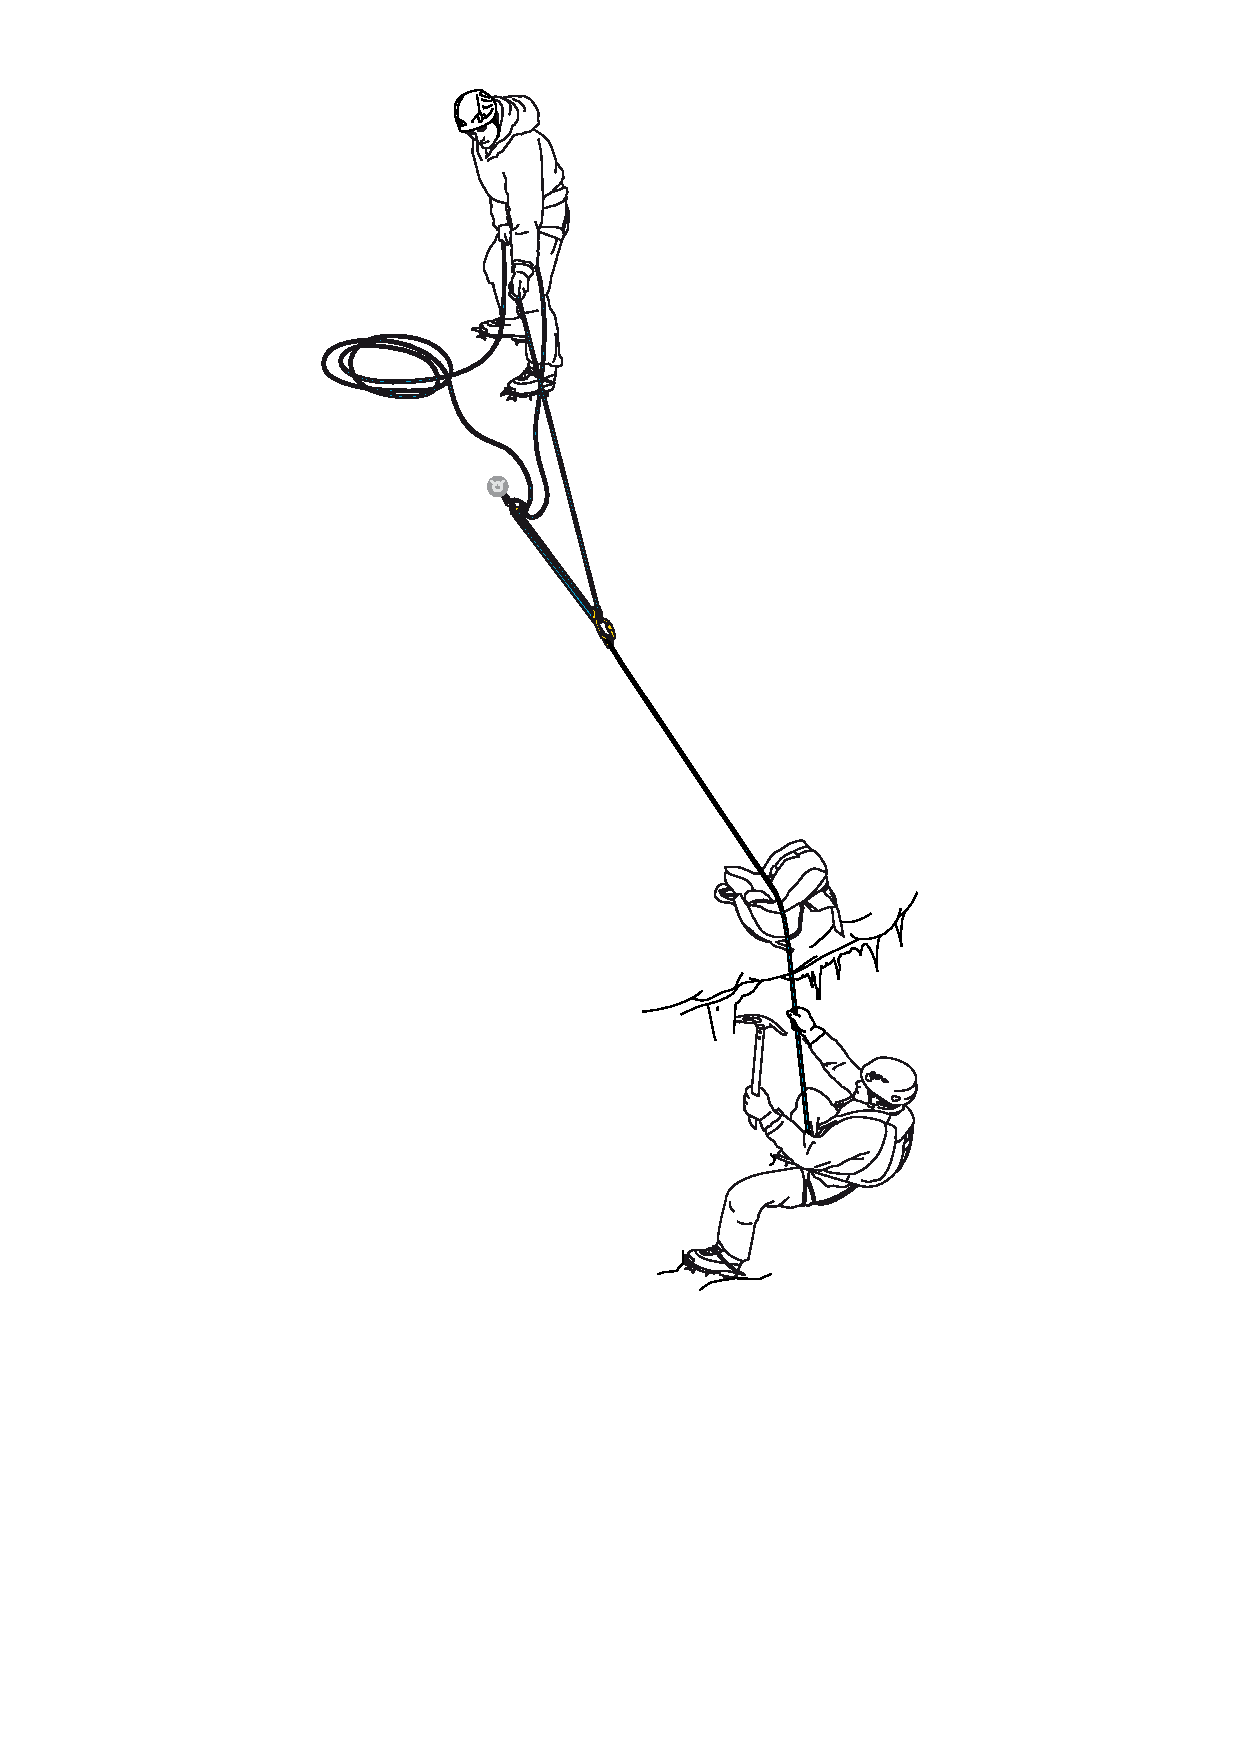
\includegraphics[width=8.0cm]{Figures/Crevasse/2_Petzl_Crevasse_haul_system_3_1.pdf}}%
    \caption[Crevasse 3:1]{Záchrana z ledovcové trhliny 3:1 (schéma převzato ze zdroje \cite{Petzl_2022})}
    \label{Obr:Crevasse_3:1}
\end{figure}
%% -------------------------------------------------- %%
%% -------------------- Pictures --------------------- %%
%% -------------------------------------------------- %%
\begin{figure}[h]
    \centering
    {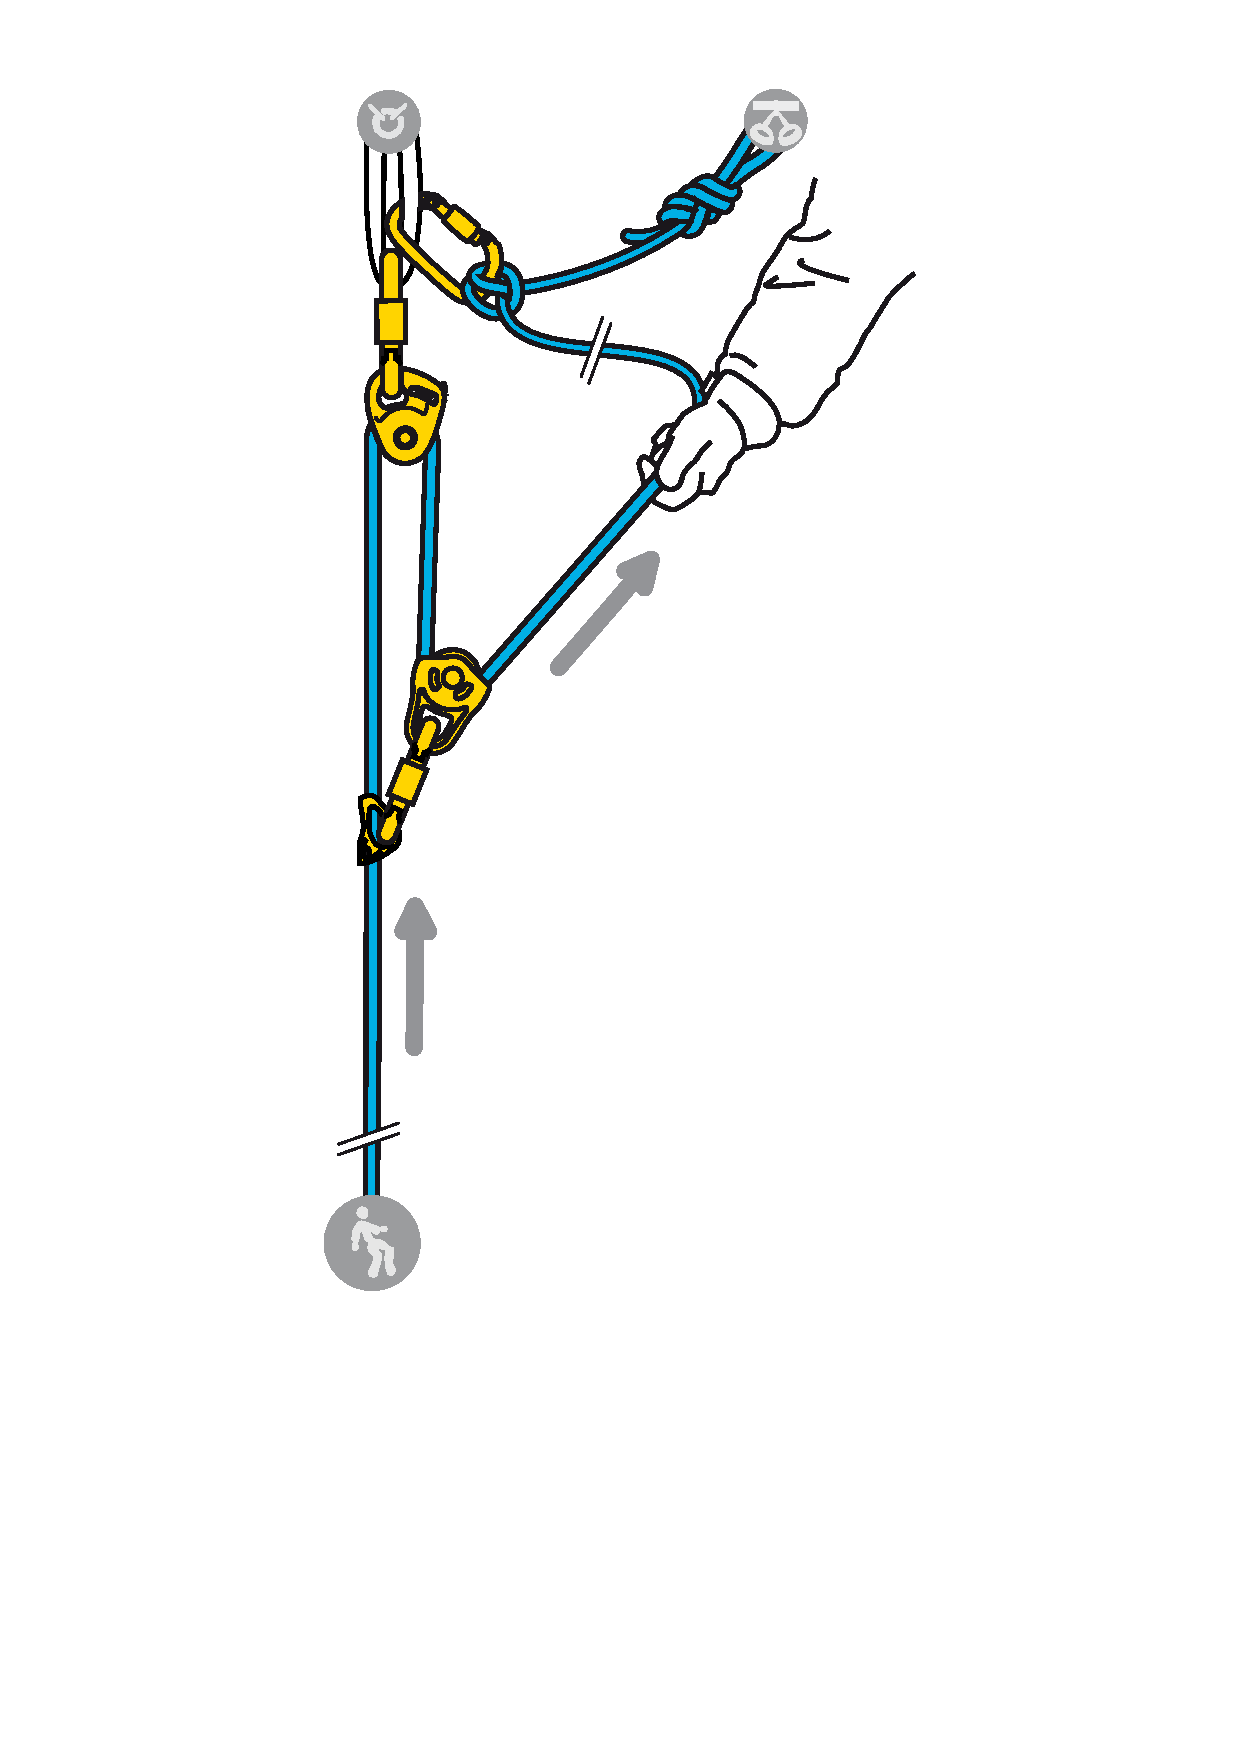
\includegraphics[width=4.0cm]{Figures/Crevasse/2_Petzl_Crevasse_haul_system_3_1_detail.pdf}}%
    \caption[Crevasse 3:1 detail]{Detail kladkostroje pro záchranu z ledovcové trhliny 3:1 (schéma převzato ze zdroje \cite{Petzl_2022})}
    \label{Obr:Crevasse_3:1_detail}
\end{figure}
%% -------------------------------------------------- %%
%% -------------------- Pictures --------------------- %%
%% -------------------------------------------------- %%
\begin{figure}[h]
    \centering
    {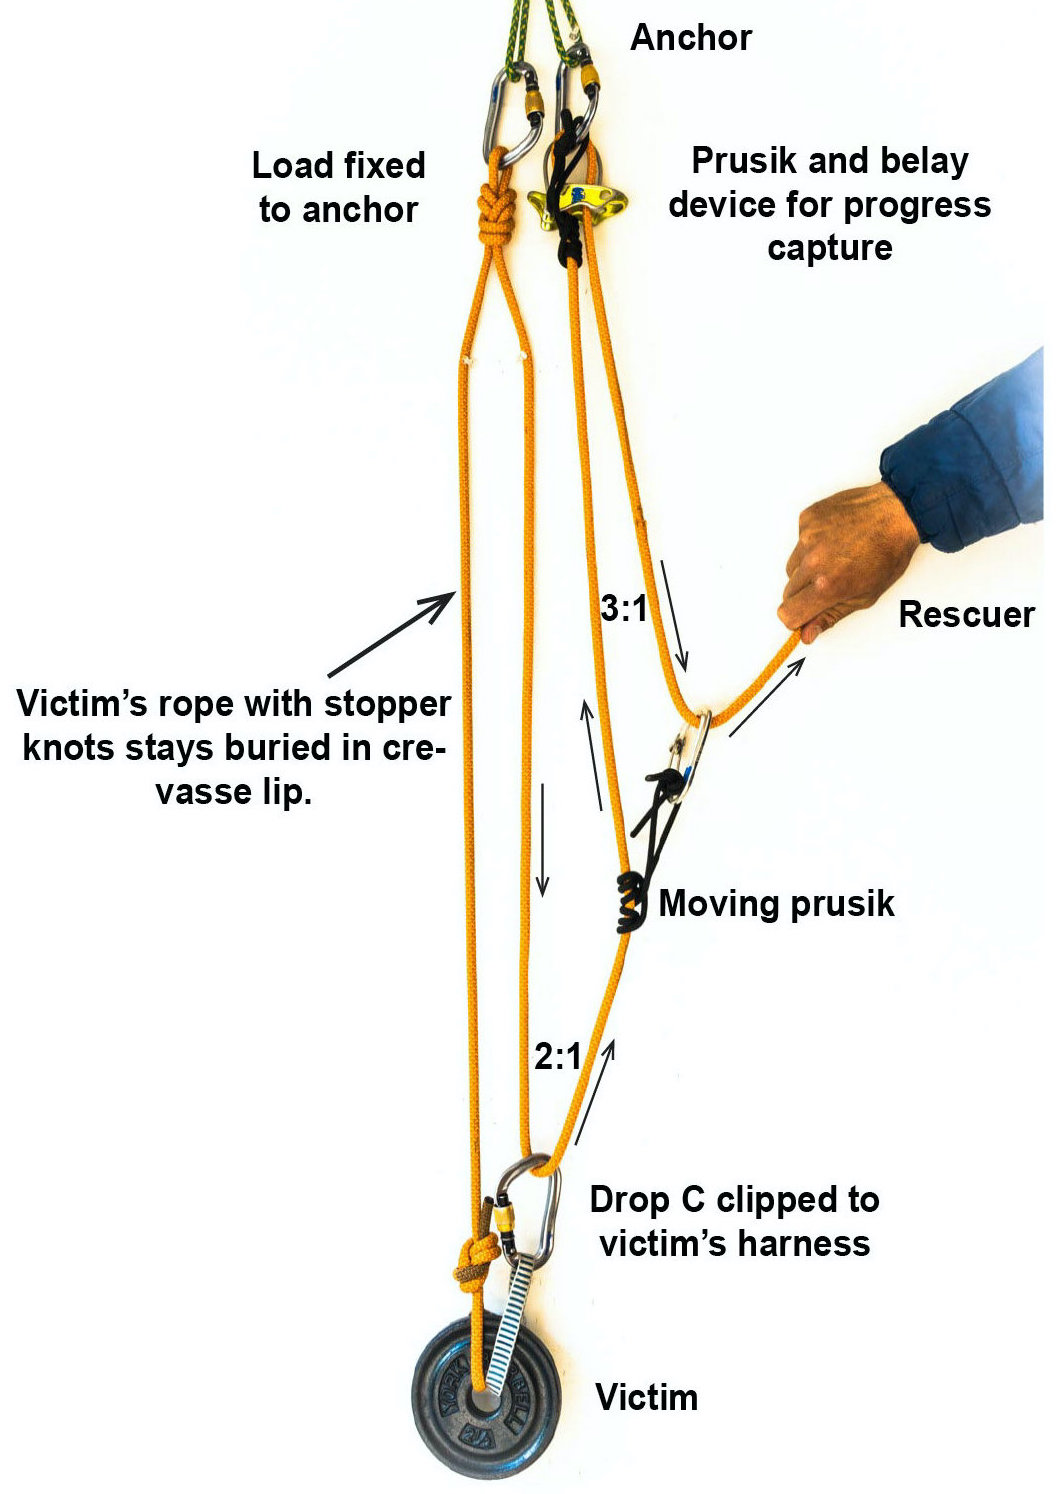
\includegraphics[width=10.0cm]{Figures/Crevasse/3_Crevasse_haul_system_6_1.jpg}}%
    \caption[Crevasse 6:1]{Záchrana z ledovcové trhliny 6:1 (schéma převzato ze zdroje \cite{stock_alpine_2022})}
    \label{Obr:Crevasse_6:1}
\end{figure}
%% -------------------------------------------------- %%
%% -------------------- Pictures --------------------- %%
%% -------------------------------------------------- %%
\begin{figure}[h]
    \centering
    {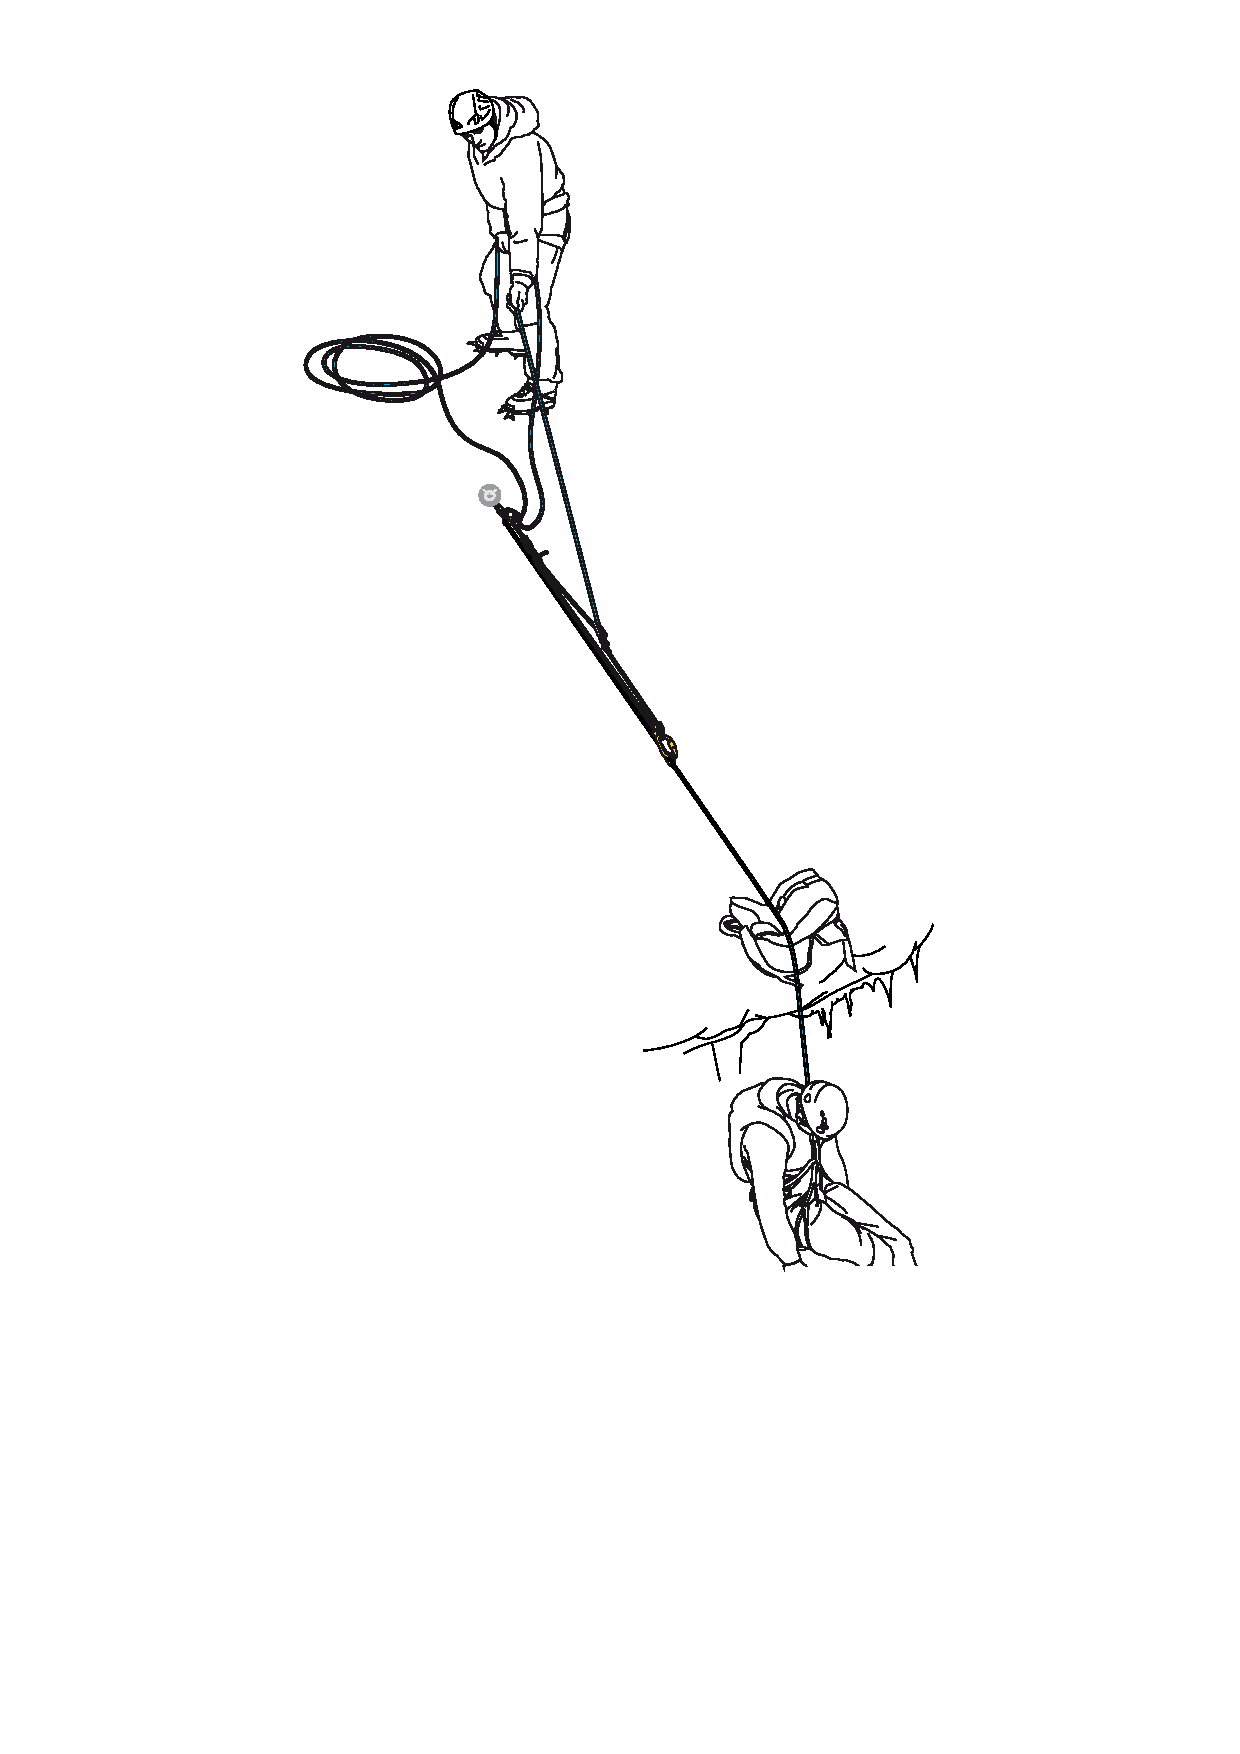
\includegraphics[width=8.0cm]{Figures/Crevasse/4_Petzl_Crevasse_haul_system_7_1.pdf}}%
    \caption[Crevasse 7:1]{Záchrana z ledovcové trhliny 7:1 (schéma převzato ze zdroje \cite{Petzl_2022})}
    \label{Obr:Crevasse_7:1}
\end{figure}
%% -------------------------------------------------- %%
%% -------------------- Pictures --------------------- %%
%% -------------------------------------------------- %%
\begin{figure}[h]
    \centering
    {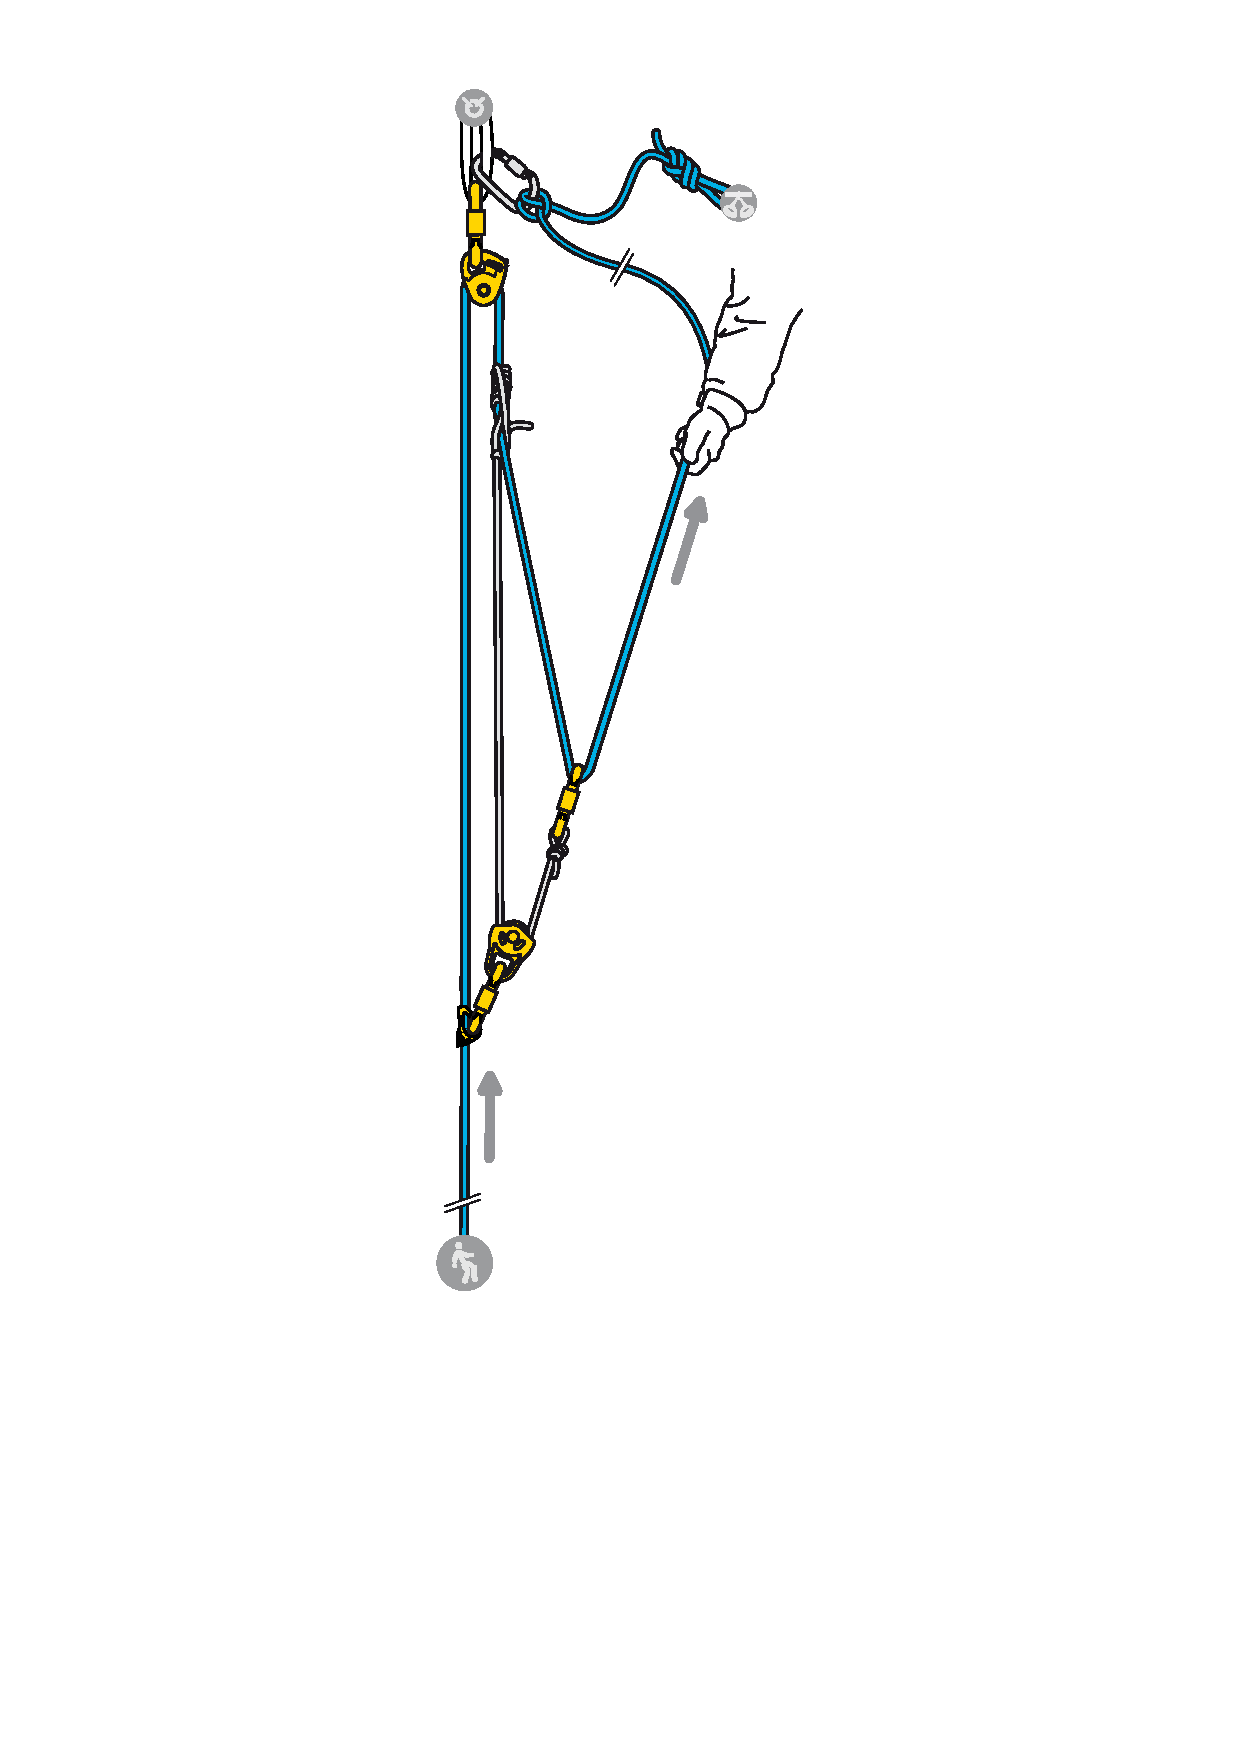
\includegraphics[width=4.0cm]{Figures/Crevasse/4_Petzl_Crevasse_haul_system_7_1_detail.pdf}}%
    \caption[Crevasse 7:1 detail]{Detail kladkostroje pro záchranu z ledovcové trhliny 7:1 (schéma převzato ze zdroje \cite{Petzl_2022})}
    \label{Obr:Crevasse_7:1_detail}
\end{figure}
%% -------------------------------------------------- %%
\subsection{Systém vytažení protiváhou "Straus"}
%% -------------------------------------------------- %%
\def\figurename{Obr.} % Figure name
\def\tablename{Tab.} % Table name
\def\figureautorefname{obr.} % Autoreference 
\def\tableautorefname{tab.} % Autoreference
\def\chapterautorefname{kapitola} % Autoreference
%% -------------------------------------------------- %%
Nejjednodušší dopomoc či vytažení vlastní váhou.
\\
\\
\textbf{Postup:}

1. Kravskou smyčkou zajistíme jístitko či půllodní uzel. 

2. Umístímě trojitý 1,5\,m prusík a zafixujeme jej ve stanovišti.

3. Zrušíme zablokované jištění a pouze lano procvakneme ve stanovišti karabinou.

4. Na volném konci lana použijeme otevřenou gardu umístěnou v centrálním oku sedacího úvazku.

5. Zatížením volného konce vlastní vahou a současným přitažením lana jdoucímu k lezci jej takto vytáhneme. Nutné vždy posunout prusík, který nám zajistí vytažené lano.
\\
\\
\textbf{Nejčastější chyby:}

1. Špatné uvázání prusíku.

2. Přeskočení prusíku v karabině, lze vyřešit umístěním reversa před prusík a zkrácením prusíku na nejmenší délku či použití tiblocu nebo microtraxtionu.

3. Neprodloužení sebejištění a tedy špatné zatěžování \cite{climbing_school_2022}.

\subsection{Expresflaschenzug}

Metoda, která spíše slouží jako pomoc druholezci v situacích, kdy se v cestě nachází těžší místo, které nemůže lezec svépomocí překonat. 
\\
\\
\textbf{Postup:}

1. Pokud dobíráme spolulezce přes reverso či půllodní uzel, zajístíme jíštění kravskou smyčkou. 

2. Na zatížené lano umístíme prusík 1,5\,m, který zkrátíme na nejmenší možnou délku a procvakneme jím karabinu.

3. Volný pramen lana protáhneme karabinou s prusíkem. Uvolníme zablokované jistítko a dobíráme lezce \cite{climbing_school_2022}.

\subsection{Seirollflaschenzug}

Nejjednodušší sestrojení kladkostroje. Technika je stejná jako u předešlé techniky Expresflaschenzug, pouze nyní zrušíme jištění a pouze lano procvakneme do karabiny. Jedná se o kladkostroj s účinností 3:1.
\\
\\
\textbf{Postup:}

1. Lezec nám visí v prusíku umístěném za půllodním uzlem. Kravskou smyčkou zajistíme půllodní uzel. 

2. Na zatížené lano umístíme prusík 1,5\,m, který zkrátíme na nejmenší možnou délku a procvakneme jím karabinu.

3. Volný pramen lana protáhneme karabinou s prusíkem. Uvolníme zablokované jistítko a zrušíme jej, lezec nám visí v pomocném prusíku. Lano z jistítka procvakneme karabinou do jistícího stanoviště \cite{climbing_school_2022}. 

\subsection{Flaschenzug}

Kladkostroj s účinností 5:1.
\\
\\
\textbf{Postup:}

1. Lezec nám visí v prusíku umístěném za půllodním uzlem. Kravskou smyčkou zajistíme půllodní uzel. 

2. Na zatížené lano umístíme prusík 1,5\,m, který zkrátíme na nejmenší možnou délku a procvkaneme jím karabinu.

3. Do jistícího stanoviště umístíme 5,0\, prusík, který provážeme skrz karabinu a protáhneme skrz karabinu s prusíkem. 

4. Karabinou protáhneme volný konec lana \cite{climbing_school_2022}.

\subsection{Kladkostroj 7:1}

Kladkostroj s účinností 7:1. 
\\
\\
\textbf{Postup:}

1. Lezec nám visí v prusíku umístěném za půllodním uzlem. Kravskou smyčkou zajistíme půllodní uzel. 

2. Na zatížené lano umístíme prusík 1,5\,m, který zkrátíme na nejmenší možnou délku a procvakneme jím karabinu.

3. Za půllodním uzlem, tedy volným koncem lana umístíme 5,0\,m prusík, který protáhneme skrz karabinu s 1,5\,m prusíkem umístěném na zatíženém laně. 

4. Do 5,0\,m prusíku procvakneme karabinu a volný konec lana.

%\selectlanguage{czech}
\chapter{Webová aplikace - Pulley systems simulation}
\label{Webova_aplikace}
%% -------------------------------------------------- %%
\def\figurename{Obr.} % Figure name
\def\tablename{Tab.} % Table name
\def\figureautorefname{obr.} % Autoreference 
\def\tableautorefname{tab.} % Autoreference
\def\chapterautorefname{kapitola} % Autoreference
%% -------------------------------------------------- %%

\section{Představení aplikace}

Vytvořila jsem webovou aplikaci, pro výpočet potřebné síly k vytažení zachraňovaného lezce (viz~\autoref{Obr:1_application}). První volbou v aplikaci je požadovaný systém kladkostroje, který se v zápětí vykreslí (viz~\autoref{Obr:6_application}). Lze zvolit kladkostroje s mechanickou účinností 3:1, 5:1 a nebo 7:1 (viz~\autoref{Obr:2_application}). Druhou volbou v aplikaci je nastavení konkrétní účinnosti jednotlivých kladek v systému (viz~\autoref{Obr:3_application}). Pokud není nastavena žádná hodnota, uvažuje se se 100\% účinností, jedná se o dokonalý stav, který v realném prostředí není možný. Pomocí posuvníku či příslušných tlačítek lze nastavit hmotnost lezce (viz~\autoref{Obr:4_application}). V neposlední řadě lze nastavit vzdálenost, kterou chceme za pomocí kladkostroje překonat (viz~\autoref{Obr:5_application}). 

%% -------------------------------------------------- %%
%% -------------------- Picture --------------------- %%
%% -------------------------------------------------- %%
\begin{figure}[!hbt]
    \centering
    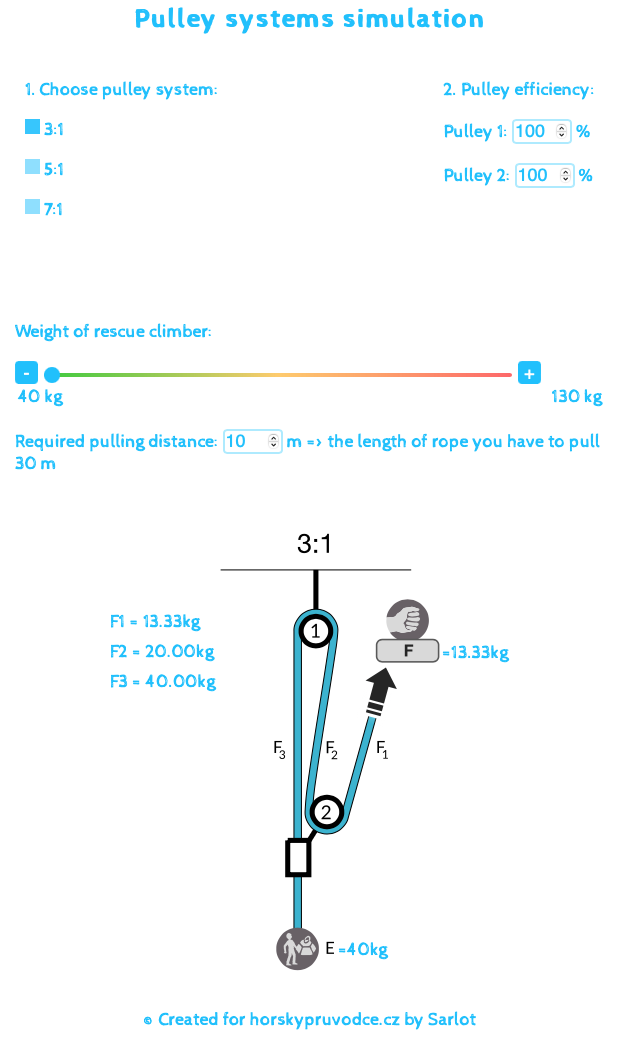
\includegraphics[width=10.0cm]{Figures/WebApplication/1_Web_application.png}
    \caption[1_Aplikace]{Kompletní zobrazení aplikace}
    \label{Obr:1_application}
\end{figure} 
%% -------------------------------------------------- %%

%% -------------------------------------------------- %%
%% -------------------- Picture --------------------- %%
%% -------------------------------------------------- %%
\begin{figure}[!hbt]
    \centering
    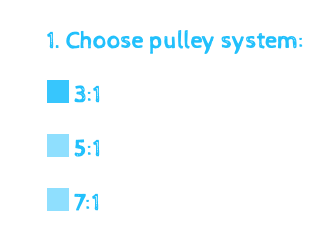
\includegraphics[width=4.0cm]{Figures/WebApplication/2_Web_application.png}
    \caption[2_Aplikace]{První volba v aplikaci - výběr kladkostroje}
    \label{Obr:2_application}
\end{figure} 
%% -------------------------------------------------- %%

%% -------------------------------------------------- %%
%% -------------------- Picture --------------------- %%
%% -------------------------------------------------- %%
\begin{figure}[!hbt]
    \centering
    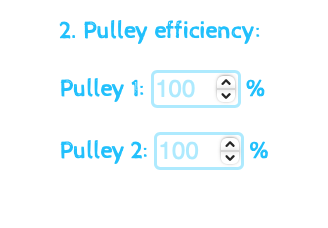
\includegraphics[width=4.0cm]{Figures/WebApplication/3_Web_application.png}
    \caption[3_Aplikace]{Možnost nastavit konkrétní hodnotu účinnosti dané kladky}
    \label{Obr:3_application}
\end{figure} 
%% -------------------------------------------------- %%

%% -------------------------------------------------- %%
%% -------------------- Picture --------------------- %%
%% -------------------------------------------------- %%
\begin{figure}[!hbt]
    \centering
    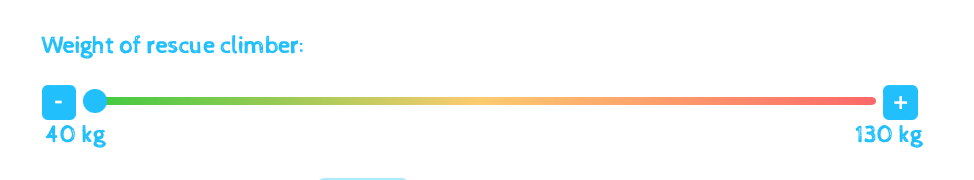
\includegraphics[width=10.0cm]{Figures/WebApplication/4_Web_application.png}
    \caption[4_Aplikace]{Nastavení hmotnosti vytahovaného lezce}
    \label{Obr:4_application}
\end{figure} 
%% -------------------------------------------------- %%

%% -------------------------------------------------- %%
%% -------------------- Picture --------------------- %%
%% -------------------------------------------------- %%
\begin{figure}[!hbt]
    \centering
    
\includegraphics[width=10.0cm]{Figures/WebApplication/5_Web_application.png}
    \caption[5_Aplikace]{Zadání požadované vzdálenosti vytahovaného lezce}
    \label{Obr:5_application}
\end{figure} 
%% -------------------------------------------------- %%

%% -------------------------------------------------- %%
%% -------------------- Picture --------------------- %%
%% -------------------------------------------------- %%
\begin{figure}[!hbt]
    \centering
    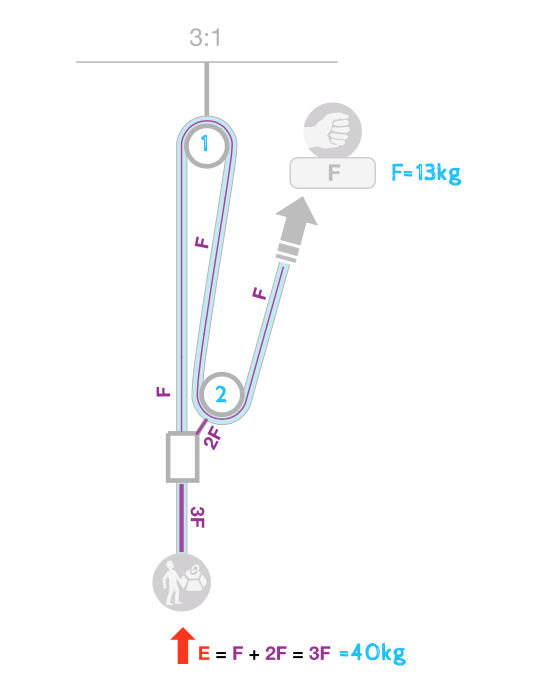
\includegraphics[width=8.0cm]{Figures/WebApplication/6_Web_application.png}
    \caption[6_Aplikace]{Schéma kladkostroje}
    \label{Obr:6_application}
\end{figure} 
%% -------------------------------------------------- %%
\chapter{Výpočty}
\label{Vypocty}
%% -------------------------------------------------- %%
\def\figurename{Obr.} % Figure name
\def\tablename{Tab.} % Table name
\def\figureautorefname{obr.} % Autoreference 
\def\tableautorefname{tab.} % Autoreference
\def\chapterautorefname{kapitola} % Autoreference
%% -------------------------------------------------- %%

\section{Výpočet síly potřebné k vytažení zachraňovaného lezce}
\subsection{Ideální kladkostroj}
V této kapitole uvedu výpočet, který je zakomponován ve webové aplikaci. Pro výpočet se 100\% účinností, tedy ideálním kladkostrojem uvažuji ve webové aplikaci v případě pokud uživatel nezadá konkrétní účinnost kladky.

\noindent Obecná rovnice síly:
%% -------------------------------------------------- %%
%% -------------------- Equation --------------------- %%
%% -------------------------------------------------- %%
\begin{equation}
    \label{eqn:basic_forces}
    S = \frac{F}{\mu \cdot n}
\end{equation}
%% -------------------------------------------------- %%
%% -------------------- Equation --------------------- %%
%% -------------------------------------------------- %%
\begin{equation}
    \label{eqn:basic_forces_2}
    S = \frac{m \cdot g}{\mu \cdot n}
\end{equation}

\begin{tabular}{l l c p{9.75cm}}
    kde: \hspace{0.25cm} & $S$ & -- & síla úsilí [N]\\
    \hspace{0.25cm} & $F$ & -- & síla zátěže [N]\\
    \hspace{0.25cm} & $m$ & -- & hmotnost zátěže [kg]\\
    \hspace{0.25cm} & $g$ & -- & gravitační konstanta $[9,80665\,m \cdot s^{-2}]$\\
    \hspace{0.25cm} & $\mu$ & -- & účinnost (rovné jedné pro ideální systém bez tření, zlomek menší než jedna u systémů v reálném světě se ztrátami energie v důsledku tření)\\
    \hspace{0.25cm} & $n$ & -- & mechanická účinnost systému\\
\end{tabular}
\\
\subsection{Kladkostroj 3:1}
Pokud uživatel zadá konkrétní účinnost kladky, uvažuji pro \textbf{systém 3:1} následující vzorec:
%% -------------------------------------------------- %%
%% -------------------- Equation --------------------- %%
%% -------------------------------------------------- %%
\begin{equation}
    \label{eqn:calculation_3_1}
    F = \frac{m}{1 + \frac{f_2}{100} \cdot (1 + \frac{f_1}{100})}
\end{equation}

\subsection{Kladkostroj 5:1}
Uvažuji rozložení sil (viz~\autoref{Obr:pulley_system_5_1}). Od pramene, kterým se vytahuje zachraňovaný se jednotlivé části lana mezi kladkami rozdělí na ${F_1}$ - ${F_5}$. Kladky označuji ${f_1}$ - ${f_4}$ a začínají s číslováním od zachraňovaného.
%% -------------------------------------------------- %%
%% -------------------- Picture --------------------- %%
%% -------------------------------------------------- %%
\begin{figure}[!hbt]
    \centering
    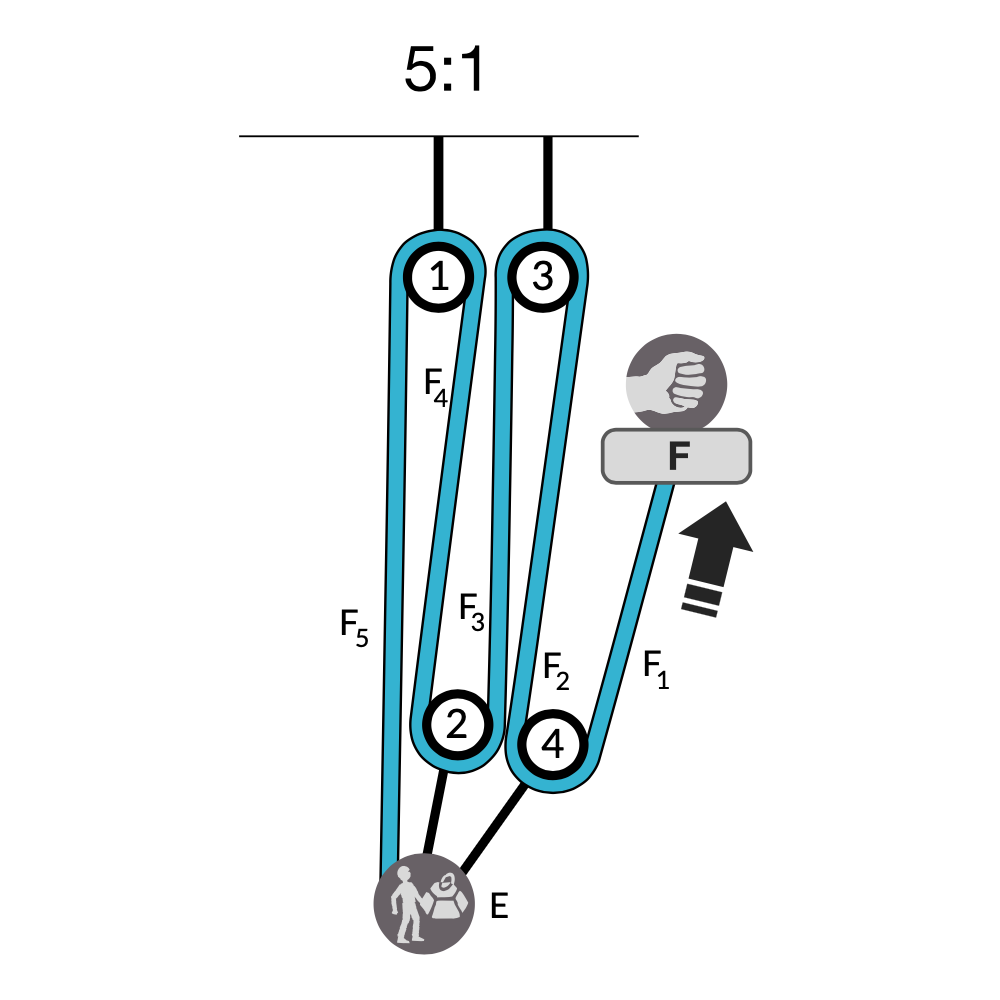
\includegraphics[width=10.0cm]{Figures/5_1/3_haul_syste_5_1_changed.png}
    \caption[Schéma kladkostroje 5:1]{Schéma kladkostroje 5:1 (schéma převzato ze zdroje \cite{Petzl_2022})}
    \label{Obr:pulley_system_5_1}
\end{figure} 
%% -------------------------------------------------- %%

\noindent Pro \textbf{systém 5:1} uvažuji následující vzorce:
%% -------------------------------------------------- %%
%% -------------------- Equation --------------------- %%
%% -------------------------------------------------- %%
\begin{equation}
    \label{eqn:9_calculation_5_1}
    F = \frac{m}{F_{celk}}
\end{equation}

\noindent Získáme následující rovnici, se kterou počítám ve webové aplikaci.
%% -------------------------------------------------- %%
%% -------------------- Equation --------------------- %%
%% -------------------------------------------------- %%
\begin{equation}
    \label{eqn:10_calculation_5_1}
    F = \frac{m}{1 + \frac{f_4}{100} \cdot (1 + \frac{f_3}{100} \cdot (1 + \frac{f_2}{100} \cdot (1 + \frac{f_1}{100})))}
\end{equation}
\subsection{Kladkostroj 7:1}
Uvažuji rozložení sil (viz~\autoref{Obr:pulley_system_7_1}). Od pramene, kterým se vytahuje zachraňovaný se jednotlivé části lana mezi kladkami rozdělí na ${F_1}$ - ${F_5}$. Kladky označuji ${f_1}$ - ${f_3}$ a začínají s číslováním od zachraňovaného.
%% -------------------------------------------------- %%
%% -------------------- Picture --------------------- %%
%% -------------------------------------------------- %%
\begin{figure}[!hbt]
    \centering
    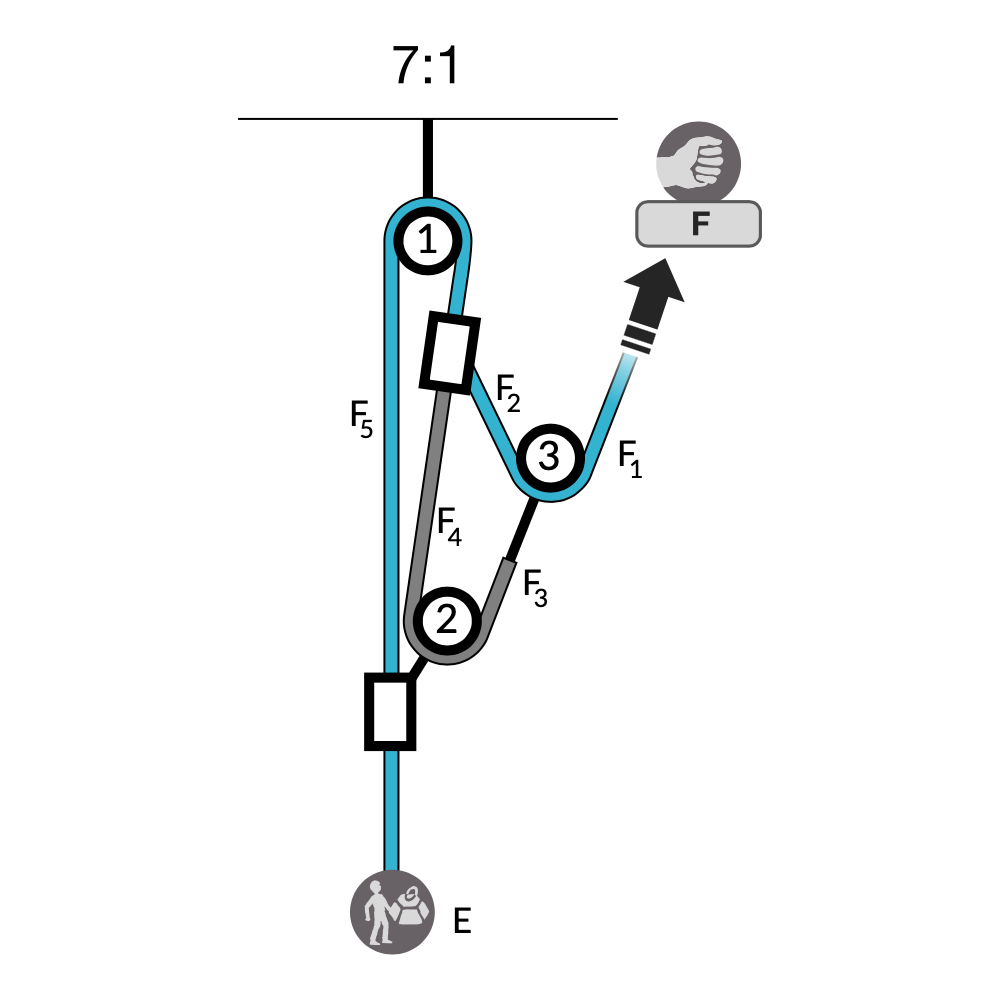
\includegraphics[width=10.0cm]{Figures/7_1/3_haul_syste_7_1_changed.png}
    \caption[Schéma kladkostroje 7:1]{Schéma kladkostroje 7:1 (schéma převzato ze zdroje \cite{Petzl_2022})}
    \label{Obr:pulley_system_7_1}
\end{figure} 
%% -------------------------------------------------- %%
\newpage
\noindent Pro \textbf{systém 7:1} uvažuji následující vzorce:
%% -------------------------------------------------- %%
%% -------------------- Equation --------------------- %%
%% -------------------------------------------------- %%
\begin{equation}
    \label{eqn:1_calculation_7_1}
    F_1 = 1
\end{equation}
%% -------------------------------------------------- %%
%% -------------------- Equation --------------------- %%
%% -------------------------------------------------- %%
\begin{equation}
    \label{eqn:2_calculation_7_1}
    F_2 = \frac{f_3}{100} \cdot F_1
\end{equation}
%% -------------------------------------------------- %%
%% -------------------- Equation --------------------- %%
%% -------------------------------------------------- %%
\begin{equation}
    \label{eqn:3_calculation_7_1}
    F_3 = F_1 + F_2
\end{equation}
%% -------------------------------------------------- %%
%% -------------------- Equation --------------------- %%
%% -------------------------------------------------- %%
\begin{equation}
    \label{eqn:4_calculation_7_1}
    F_4 = \frac{f_2}{100} \cdot F_3
\end{equation}
%% -------------------------------------------------- %%
%% -------------------- Equation --------------------- %%
%% -------------------------------------------------- %%
\begin{equation}
    \label{eqn:5_calculation_7_1}
    F_5 = \frac{f_1}{100} \cdot (F_2 + F_4)
\end{equation}
%% -------------------------------------------------- %%
%% -------------------- Equation --------------------- %%
%% -------------------------------------------------- %%
\begin{equation}
    \label{eqn:6_calculation_7_1}
    E = F_3 + F_4 + F_5
\end{equation}

\noindent Po dosazení do rovnice:
%% -------------------------------------------------- %%
%% -------------------- Equation --------------------- %%
%% -------------------------------------------------- %%
\begin{equation}
    \label{eqn:7_calculation_7_1}
    F_{celk} = (F_1 + F_2) + (\frac{f_2}{100} \cdot F_3) + (\frac{f_1}{100} \cdot (F_2 + F_4))
\end{equation}

\noindent Získáme následující rovnici:
%% -------------------------------------------------- %%
%% -------------------- Equation --------------------- %%
%% -------------------------------------------------- %%
\begin{equation}
    \label{eqn:8_calculation_7_1}
    F_{celk} = (1 + \frac{f_3}{100} \cdot 1) + (\frac{f_2}{100} \cdot (1 + (\frac{f_3}{100} \cdot 1))) + (\frac{f_1}{100} \cdot ((\frac{f_3}{100} \cdot 1) + (\frac{f_2}{100} \cdot (1 + (\frac{f_3}{100} \cdot 1)))))
\end{equation}

\noindent Dostávám následující rovnici, se kterou počítám ve webové aplikaci.
%% -------------------------------------------------- %%
%% -------------------- Equation --------------------- %%
%% -------------------------------------------------- %%
\begin{equation}
    \label{eqn:9_calculation_7_1}
    F = \frac{m}{F_{celk}}
\end{equation}

%% -------------------------------------------------- %%
%% -------------------- Equation --------------------- %%
%% -------------------------------------------------- %%
\begin{equation}
    \label{eqn:10_calculation_7_1}
    F = \frac{m}{(1 + \frac{f_3}{100} \cdot 1) + (\frac{f_2}{100} \cdot (1 + (\frac{f_3}{100} \cdot 1))) + (\frac{f_1}{100} \cdot ((\frac{f_3}{100} \cdot 1) + (\frac{f_2}{100} \cdot (1 + (\frac{f_3}{100} \cdot 1)))))}
\end{equation}

\begin{tabular}{l l c p{9.75cm}}
    kde: \hspace{0.25cm} & $F$ & -- & vytahovaná hmotnost zachraňovaného lezce [kg]\\
    \hspace{0.25cm} & $m$ & -- & hmotnost vytahovaného lezce [kg]\\
    \hspace{0.25cm} & $F_1$ - $F_5$ & -- & mezivýpočet účinnosti systému [\%]\\
    \hspace{0.25cm} & $f_1$ - $f_4$ & -- & účinnost kladkostroje [\%]\\
\end{tabular}
\\
\section{Výpočet vytažené délky lana k zachránění lezce o požadovanou vzdálenost}
Při výpočtu vycházím z již vypočtených účinností systému $F_{celk}$.
%% -------------------------------------------------- %%
%% -------------------- Equation --------------------- %%
%% -------------------------------------------------- %%
\begin{equation}
    \label{eqn:calculation_distance}
    l = l_{poz} \cdot F_{celk}
\end{equation}

\begin{tabular}{l l c p{9.75cm}}
    kde: \hspace{0.25cm} & $l$ & -- & skutečná vytažená délka lana k zachraně lezce o požadovanou vzdálenost [m]\\
    \hspace{0.25cm} & $l_{poz}$ & -- & požadovaná vzdálenost k vytažení zachraňovaného lezce [m]\\
    \hspace{0.25cm} & $F_{celk}$ & -- & celkový výpočet účinnosti systému [\%]\\
\end{tabular}
\chapter{Příklady účinností kladkostroje}
\label{Souhrn}
%% -------------------------------------------------- %%
\def\figurename{Obr.} % Figure name
\def\tablename{Tab.} % Table name
\def\figureautorefname{obr.} % Autoreference 
\def\tableautorefname{tab.} % Autoreference
\def\chapterautorefname{kapitola} % Autoreference
%% -------------------------------------------------- %%

V systému kladkostroje mohou být zabudovány pomůcky jako je například micro traxion, který má účinnost 91\%, taktéž kladka s valivými ložisky má stejnou účinnost. Pozor na kladku s kluznými ložisky, ta má nižší účinnost, která se může pohybovat okolo 71\%. Pokud do systému zavedeme karabinu bude účinnost mezi 50-60\%.


\section{Kladkostroj 3:1}

\begin{table}[h!] % Will place table here approximately
    \begin{tabular}{|c|c|c|}
        \hline
        \multicolumn{1}{|l|}{kladka č.1} & \multicolumn{1}{l|}{kladka č.2} & \multicolumn{1}{l|}{kladkostroj} \\ \hline
        {účinnost [}\%{]}                & {účinnost [}\%{]}               & 3:1                              \\ \hline
        50                               & 50                              & 1,75:1                           \\ \hline
        91                               & 50                              & 1,96:1                           \\ \hline
        91                               & 91                              & 2,74:1                           \\ \hline
    \end{tabular}
\end{table}

\section{Kladkostroj 5:1}

\begin{table}[h!]
    \begin{tabular}{|c|c|c|c|c|}
        \hline
        kladka č.1 & kladka č.2 & kladka č.3 & kladka č.4 & kladkostroj \\ \hline
        {účinnost [}\%{]}   & {účinnost [}\%{]}   & {účinnost [}\%{]}   & {účinnost [}\%{]}   & 5:1         \\ \hline
        50                  & 50                  & 50                  & 50                  & 1,94:1      \\ \hline
        91                  & 50                  & 50                  & 50                  & 1,99:1      \\ \hline
        50                  & 91                  & 50                  & 50                  & 2,09:1      \\ \hline
        50                  & 50                  & 91                  & 50                  & 1,94:1      \\ \hline
        50                  & 50                  & 50                  & 91                  & 2,71:1      \\ \hline
        91                  & 91                  & 50                  & 50                  & 1,99:1      \\ \hline
        91                  & 50                  & 91                  & 50                  & 2,39:1      \\ \hline
        91                  & 50                  & 50                  & 91                  & 2,80:1      \\ \hline
        50                  & 91                  & 91                  & 50                  & 2,58:1      \\ \hline
        50                  & 91                  & 50                  & 91                  & 2,99:1      \\ \hline
        50                  & 50                  & 91                  & 91                  & 3,36:1      \\ \hline
        91                  & 91                  & 91                  & 50                  & 2,75:1      \\ \hline
        91                  & 50                  & 91                  & 91                  & 3,53:1      \\ \hline
        91                  & 91                  & 50                  & 91                  & 3,16:1      \\ \hline
        50                  & 91                  & 91                  & 91                  & 3,87:1      \\ \hline
        91                  & 91                  & 91                  & 91                  & 4,18:1      \\ \hline
    \end{tabular}
\end{table}
\newpage
\section{Kladkostroj 7:1}

\begin{table}[h!]
    \begin{tabular}{|c|c|c|c|}
        \hline
        kladka č.1 & kladka č.2 & kladka č.3 & kladkostroj \\ \hline
        {účinnost [}\%{]}   & {účinnost [}\%{]}   & {účinnost [}\%{]}   & 7:1         \\ \hline
        50                  & 50                  & 50                  & 2,88:1      \\ \hline
        91                  & 50                  & 50                  & 3,39:1      \\ \hline
        50                  & 91                  & 50                  & 3,80:1      \\ \hline
        50                  & 50                  & 91                  & 3,80:1      \\ \hline
        91                  & 91                  & 50                  & 4,56:1      \\ \hline
        91                  & 50                  & 91                  & 4,56:1      \\ \hline
        50                  & 91                  & 91                  & 4,98:1      \\ \hline
        91                  & 91                  & 91                  & 6,06:1      \\ \hline
    \end{tabular}
\end{table}
\chapter*{Závěr}
\addcontentsline{toc}{chapter}{Závěr}
\fancyhead{}
%% -------------------------------------------------- %%
\def\figurename{Obr.} % Figure name
\def\tablename{Tab.} % Table name
\def\figureautorefname{obr.} % Autoreference 
\def\tableautorefname{tab.} % Autoreference
\def\chapterautorefname{kapitola} % Autoreference
%% -------------------------------------------------- %%

V úvodu práce byl popsán základní materiál potřebný k záchraně spolulezce či klienta. Dále jsem se zaměřila na základní záchranné techniky klientů ve volném terénu či na zajištěných cestách. Popsala jsem kladkový efekt a uvedla kladkostroje se systém 1:1, 2:1, 3:1, 4:1, 5:1, 7:1. Stručně jsem popsala provedení nejčastěji používaných kladkostrojů. 

Výstupem této práce bylo vytvořit webovou aplikaci, kde si uživatel bude moct nastavit hmotnost zachraňovaného lezce, zavést do výpočtu různé případy účinnosti kladek použitých v systému a umožní vypočítat skutečnou vytaženou délku lana k záchraně lezce o požadovanou vzdálenost. Všechny výpočty ve webové aplikaci byly shrnuty v kapitole zaměřené na výpočet.

Cílem této aplikace je umožnit uživateli jednoduše nasimulovat situaci a vypočítat jakou hmotnost bude muset vytáhnout, pokud jeho spolulezec či klient nebude moct překonat určitou pasáž, či se zraní a nebude moct pokračovat ve výstupu. 

Samozřejmě záleží na mnoha dalších vlivech, které v aplikaci nejsou uvažovány. Výsledek je tedy pouze orientační. V realném případě bude mít vliv na výslednou sílu tloušťka lana, protažení prusíku, vlhkost lana či opotřebení pomůcek zakomponovaných v systému. Také bude mít vliv na výslednou sílu úhel, pod kterým bude lano vytahováno, to samozřejmě bude záviset na pracovním prostoru. 

\begin{comment}
%% -------------------------------------------------- %%
%% ----------------- List of figures ------------------ %%
%% -------------------------------------------------- %%
\newpage
\addcontentsline{toc}{chapter}{Seznam obrázků}
\renewcommand{\listfigurename}{Seznam obrázků}
\renewcommand{\cftloftitlefont}{\fontsize{16}{10}\selectfont\color{NavyBlue}}
\setlength{\cftafterloftitleskip}{10pt}
\clearpage % Otherwise \pagestyle affects the previous page.
{% Enclosed in braces so that re-definition is temporary.
  \pagestyle{empty} % Removes numbers from middle pages.
  \fancypagestyle{plain} % Re-definition removes numbers from first page.
  {%
    \fancyhf{} % Clear all header and footer fields.
    \renewcommand{\headrulewidth}{0pt} % Clear rules (remove these two lines if not desired).
    \renewcommand{\footrulewidth}{0pt}%
  }
 	{%
	\let\oldnumberline\numberline%
	\renewcommand{\numberline}{Obr.~\oldnumberline}%
	\listoffigures%
	}
  \thispagestyle{empty} % Removes numbers from last page.
}
\end{comment}
%% -------------------------------------------------- %%
%% ---------------- List of equations ---------------- %%
%% -------------------------------------------------- %%
\newpage
\addcontentsline{toc}{chapter}{Seznam rovnic}
\listofmyequations
\thispagestyle{empty}
%% -------------------------------------------------- %%
%% ------------------ Bibliography ------------------- %%
%% -------------------------------------------------- %%
\newpage
\addcontentsline{toc}{chapter}{Seznam použité literatury}
\clearpage % Otherwise \pagestyle affects the previous page.
{% Enclosed in braces so that re-definition is temporary.
  \pagestyle{empty} % Removes numbers from middle pages.
  \fancypagestyle{plain} % Re-definition removes numbers from first page.
  {%
    \fancyhf{} % Clear all header and footer fields.
    \renewcommand{\headrulewidth}{0pt} % Clear rules (remove these two lines if not desired).
    \renewcommand{\footrulewidth}{0pt}%
  }
  \bibliographystyle{BibDesk/czechiso.bst} % Plain is another style
 % \begin{flushleft}
 \Urlmuskip=0mu plus 1mu\relax
  \bibliography{BibDesk/Bibliography}
  %\end{flushleft}
  \thispagestyle{empty} % Removes numbers from last page.
}
\end{document}